%%%%%%%%%%%%%%%%%%%%%%%%%%%%%%%%%%%%%%%%%%%%%%%%%
%
%	MSc THESIS TEMPLATE
%	developed for my master thesis at the Universitá di Torino
%
%	by Eugenio Senes (eugenio.senes@gmail.com)
%
%	released under MIT license, so share, modify and enjoy, but quoting the author !
%
%%%%%%%%%%%%%%%%%%%%%%%%%%%%%%%%%%%%%%%%%%%%%%%%%

%% DOCUMENT CLASS (alternative to book is 'report')
% Print just right page or both sides (comment the other one)
\documentclass[12pt,a4paper,openright,oneside]{book}	%%One sided
%\documentclass[12pt,a4paper,openright,twoside]{book}	%%Double sided

\usepackage[most]{tcolorbox}
\usepackage{amsthm}
\usepackage{wrapfig}
\usepackage[inline]{enumitem}


%% SET MARGINS OF THE PAGES
\usepackage{geometry}
\geometry{a4paper,portrait, left=20mm, right=20mm, top=15mm, bottom=15mm}
\usepackage[section]{placeins}
%% HEADERS AND FOOTERS
\usepackage{fancyhdr}
\pagestyle{fancy}
\fancyhf{} 			%clears default header and footer
\rhead{} 			%right head
\lhead{ \leftmark} 	%left head
\rfoot{\thepage}
%%consider using also chead, cfoot, lfoot
%coherce the plain stile to this (e.g. the first page of every chapter)
\fancypagestyle{plain}{
	\fancyhf{}
	\rfoot{\thepage}
	\renewcommand{\headrulewidth}{0pt}
	\renewcommand{\footrulewidth}{0pt}
}
%% CLEAR PAGE WITHOUT NUMBER AT THE BEGINNING OF CHAPTERS
\let\origdoublepage\cleardoublepage
\newcommand{\clearemptydoublepage}{%
  \clearpage
  {\pagestyle{empty}\origdoublepage}%
}
%% ALLOW PAGE ROTATION
\usepackage{lscape}

%% HYPERTEXT SETUP
\usepackage{hyperref}
\hypersetup{
    colorlinks,
    citecolor=black,
    filecolor=black,
    linkcolor=black,
    urlcolor=black
}
%% PDF SETTINGS
\hypersetup{
    pdfauthor={AuthorName},
    pdftitle={shortTitle},
    pdfsubject={subject},
    pdfkeywords={keyword1, keyword2}
}
%% FONTS AND SYMBOLS
\usepackage[utf8]{inputenc}
\usepackage{amsfonts}		%%fonts for the mathematical rendering of formulas
\usepackage{amssymb}
\usepackage{amsmath}
%% CHAPTERS STRUCTURE
\usepackage[italian]{babel} %%Set English as main language of the document
%% FIGURES
\usepackage{graphicx}
\usepackage{subfigure}		%%allow side by side figures with single caption
%% TABLES
\usepackage{multirow}		%%allow to merge rows in the tables
\usepackage{booktabs}		%%allow use of \toprule, \midrule, \bottomrule in tables
%%CAPTIONS
\usepackage{caption}
%% BIBLIOGRAPHY
\usepackage[babel]{csquotes}
%% CODE LISTINGS
\usepackage{listings}		%%allow to use code listings
\usepackage{algpseudocode}
\usepackage{algorithm}

%%%%%%%%%%%%%%%%%%%%%%%%%%%%%%%%%%%%%%%%%%%%%%%%%
%%%% BEGIN DOCUMENT
\begin{document}

%%%%%% HEAD  OF THE DOCUMENT
\frontmatter
%%FRONT PAGE
\begin{titlepage}
%upper part
\begin{center}
{{\Large{\textsc{Universit\`a degli studi di Torino \\}}}} \vspace{5mm} {\small{\bf SCUOLA DI SCIENZE DELLA NATURA\\ \vspace{3mm}
Corso di Laurea Magistrale in Informatica}}
\vspace{5mm}
\end{center}
%logo
\begin{center}

\includegraphics[scale=.3]{head/logo.png}
\end{center}
%title
\begin{center}
\vspace{5mm}
{\LARGE{\bf Appunti del corso di Reti neurali e Deep Learning}}
%{\LARGE{\bf SECOND ROW TITLE}}
\end{center}
\hfill
\begin{minipage}[t]{0.47\textwidth}\raggedleft
\vspace{20mm}
{\large{\bf Autori:\\
Falchi Lorenzo\\
Picone Corrado (come il comico)}}
\end{minipage}
\vspace{10mm}
\begin{center}
{\large{\bf 
Anno Accademico 2024/2025}}
\end{center}

\end{titlepage}
\newpage\null\thispagestyle{empty}\newpage

%\begin{titlepage}
%upper part
\begin{center}
{{\Large{\textsc{Universit\`a degli studi di Torino \\}}}} \vspace{5mm} {\small{\bf SCUOLA DI SCIENZE DELLA NATURA\\ \vspace{3mm}
Corso di Laurea Magistrale in Fisica}}
\vspace{5mm}
\end{center}
%logo
\begin{center}

\includegraphics[scale=.3]{head/logo.png}
\end{center}
%title
\begin{center}
\vspace{5mm}
{\large{\bf Tesi di Laurea Magistrale\\}}
\vspace{5mm}
{\LARGE{\bf THE FANCY TITLE\\ OF MY FANCY THESIS\\}}
%\vspace{5mm}
%{\LARGE{\bf SECOND ROW TITLE}}
\end{center}
\vspace{20mm}
%reatori e candidato
\vspace{11mm}
\par
\noindent
\begin{minipage}[t]{0.47\textwidth}
{\large{\bf Relatore:\\
Prof. Zio Paperone}}\\
\vspace{4mm}
\\
{\large{\bf Correlatore:\\
Dr. Pico de Paperis (PAP) }}
\vspace{8mm}
{\large{\bf \\ Controrelatore:\\
Prof.ssa Nonna Papera}}
\end{minipage}
\hfill
\begin{minipage}[t]{0.47\textwidth}\raggedleft
\vspace{16mm}
{\large{\bf Candidato:\\
Paperoga}}
\end{minipage}
\vspace{9mm}
\begin{center}
{\large{\bf 
Anno Accademico 20xx/20xx}}
\end{center}

\end{titlepage}
%%INDEXES
%summary
\textit{Questi appunti sono basati sulle slide del corso di Reti neurali e deep learning tenuto dai professori Valentina Gliozzi e Roberto Esposito per l'anno accademico 2024/2025. Questo documento è il risultato dell'integrazione di slide e appunti presi a lezione. Ogni capitolo corrisponde a circa una lezione, quando possibile le lezioni sono accorpate in un singolo capitolo.}
\tableofcontents


%%%%%% BODY OF THE DOCUMENT
\mainmatter
%%INTRODUCTION
 \chapter{Introduzione}
\section{Machine learning}

\subsection{Task}
Le \textbf{reti neurali} sono una delle modalità con cui si possono risolvere problemi di \textbf{machine leaning}. Il machine learning è una branca dell'informatica che si occupa di come i computer apprendono e migliorano i propri risultati "imparando" dai loro stessi errori. I computer vengono in particolare applicati a \textbf{task}, i quali possono essere di diversi tipi (classificazione, regressione, clustering, ecc..).

Breve descrizione di alcuni tipi di task:

\begin{itemize}
    \item \textbf{classification}, il task di classificazione è un task \textbf{supervisionato}, il che vuol dire che a partire dalla descrizione e soluzione al problema (training set etichettato), vogliamo imparare un algoritmo di machine learning che crei un modello che risolva task di classificazione del tipo desiderato, in maniera autonoma. In particolare \textbf{il modello deve essere in grado di generalizzare} e predirre correttamente la classe di esempi che non ha visto nella fase di training (esempi: spam detection, sentiment analysis ecc..).
    \item \textbf{regression}, il task di regressione è simile a quello di classifazione, ma invece di predirre un set di lable l'output sarà un numero reale (esempi: house price prediction, stock price prediction ecc..). Si può usare un regressore per fare classificazione.
\end{itemize}


\subsection{No free launch theorem}
In sostanza, questo teorema afferma che a meno di non considerare i bias, gli algoritmi di machine learning sono sostanzialmente uguali in termini di prestazioni.

\subsection{Training di una rete neurale}
Le reti neurali sono una famiglia di incredibilmente flessibili modelli i quali riescono ad approssimare sostanzialmente qualsiasi funzione. Il prezzo da pagare è l'elevatissimo numero di iper parametri grazia ai quali si possono raggiungere ottime performance. Alcuni tipi di iper parametri sono:
\begin{itemize}
    \item numero di layer;
    \item numero di neuroni in ogni layer;
    \item learning rate;
    \item optmizer;.
    \item ....
\end{itemize}


Importantissimo è imparare a settare questi parametri e validare la qualità del modello. Ora ci concentreremo su questi due argomenti.


Il \textbf{generalization error} è l'errore che la nostra funzione \textbf{g} commette quando vede nuovi esempi, è scritta così:
\begin{equation}
    R=E_{(x,y)\sim p^*[L(y,g(x;\Theta))]}
\end{equation}
dove $p^*$ è la \textbf{reale distribuzione dei dati} e 
\begin{equation}
    L(y,g(\cdot;\Theta))
\end{equation}
è la \textbf{loss function} usata per misurare quanto vale l'errore quando $y$ è predetto come $g(x;\Theta)$.

Il problema è che qui $R$ \textbf{non è veramente calcolabile}, non si può fare praticamente. Questo perchè non abbiamo accesso a $p^*$ e anche se ce l'avessimo dovremmo valutare un numero infinito di punti, cosa che non è possibile ovviamente.

Esempi di \textbf{loss function} sono la \textbf{$0-1$ loss}:
\begin{equation}
    L(y,y')=\mathbb{I}_{y\neq y'}=
    \begin{cases}
      1 \text{ if } y\neq y'\\
      0 \text{ otherwise}
    \end{cases}\,
\end{equation}
e la \textbf{quadratic loss}:
\begin{equation}
    L(y,y')=(y-y')^2.
\end{equation}


Tornando a noi, vogliamo misurare il \textbf{generalization error} ma come abbiamo detto ciò richiede un sampling dalla distrubuzione che noi non abbiamo. Per ovviare a questo problema adotteremo diverse soluzioni, la prima è l'utilizzo di un errore diverso dal generalization, un errore più generale detto \textbf{empirical error}:
\begin{equation}
    \hat{R}_T=\dfrac{1}{|T|}\sum_{(x,y)\in T}L(y,g(x;\Theta)),
\end{equation}
dove $T$ è un campione finito estratto da $p^*$.


Arrivati a questo punto:
\begin{itemize}
    \item se  $T$ denota il \textbf{training set}, allora  $T \equiv Tr, \hat{R}_Tr$ denota il \textbf{training error} di $g$,
    \item se  $T$ denota il \textbf{test set}, allora  $T \equiv Te , \hat{R}_Te$ denota il \textbf{test error} di $g$.
\end{itemize}

Siccome il \textbf{training error} è ottimizzato semplicemente con l'algoritmo di apprendimento, ha un \textbf{bias ottimistico} (tende ad essere minore del generalization error). Quindi è sostanzialmente un estimatore ottimistico del generalization error.


Il \textbf{test error} è invece un estimatore \textbf{unbiased} del generalization error $R$, anche se a determinate condizioni il bias può essere \textbf{pessimistico}, per esempio nel caso in cui si tenga da parte una parte del training set (si immagina che trainare il modello una seconda volta utilizzando tutto il training set produca un modello con un errore minore). 


Quando si verifica che l'errore sul test set è maggiore di quello sul training set, cioè
\begin{equation}
    \hat{R}_{Te}-\hat{R}_{Tr} > 0
\end{equation}
si parla di \textbf{overfitting}. A parole, un modello soffre di overfitting quando le prestazioni sul training set sono molto migliori di quelle sul test set. Un leggero overfitting è invece abbastanza normale e tollerabile ma si tende a renderlo più piccolo possibile.\newpage

Tornando invece all'altro dei quesiti inziali, cioè \textbf{come stimare gli iperparametri}; con quello che abbiamo imparato fino ad ora, vogliamo implementare questa procedura: \newline
    redqui ci va il codice python\newline


Sfortunatamente non funziona, per sostanzialmente lo stesso motivo per cui il training è un estimatore ottimistico del generalization erorre, stiamo rendendo anche il test error un estimatore ottimistico. Così facendo stiamo portando il modello a fare overfitting sul test set.



\section{(Matrici e vettori) Calcolo}
\subsection{Derivate}
Data la funzione $y=f(x)$, dove $x$ e $y$ sono numeri reali.
La \textbf{derivata} di $f$ nel punto $x$, denotata da $f'(x)$ or $\frac{df}{dx}(x)$ è la \textbf{pendenza della tangente (o coefficiente angolare)} ad $f$ nel punto $x$.
\begin{figure}[h]
    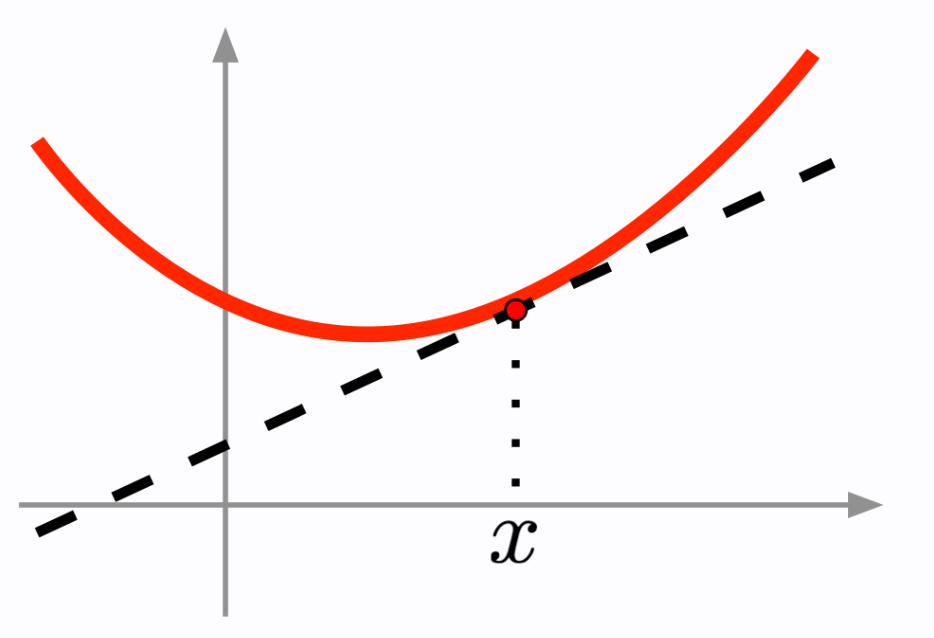
\includegraphics[scale=0.5]{images/prerequisites/derivative.png}
    \centering
\end{figure}
Tra le cose interessanti della derivata c'è il fatto che se si vuole calcolare il valore di $f$ in un punto vicino ad $x$, diciamo $\epsilon$, si può fare in questo modo:
\begin{equation}
    f(x+\epsilon) \approx f(x)+\epsilon f'(x).
\end{equation}

\textbf{Proprietà importanti delle derivate}:
\begin{itemize}
    \item \textbf{linearity} $( \alpha f(x)+ \beta g(x))' = \alpha f'(x)+\beta g'(x)$
    \item \textbf{chain rule} $(f(g(x)))' = f'(g(x))g'(x)$
    \item \textbf{prduct rule} $(g(x)h(x))' = g'(x)h(x)+g(x)h'(x)$
    \item \textbf{quotient rule} $(\frac{f(x)}{g(x)}) = \frac{f(x)'g(x)-f(x)g'(x)}{(g(x))^2}$
    \item \textbf{power rule} $(x^r)' = rx^{r-1}$
\end{itemize}
\newpage
\subsection{Integrali}
Data la funzione $f:\mathbb{R} \rightarrow \mathbb{R}$ e un intervallo $[a,b]$ sulla retta reale: \newline
\textbf{l'integrale di $f$ tra $a$ e $b$ rappresenta l'area sotto $f$ nella regione delimitata dagli estremi dell'intervallo} (quando la funzione si trova sotto lo 0, l'area contribuisce negativamente).
\begin{figure}[h]
    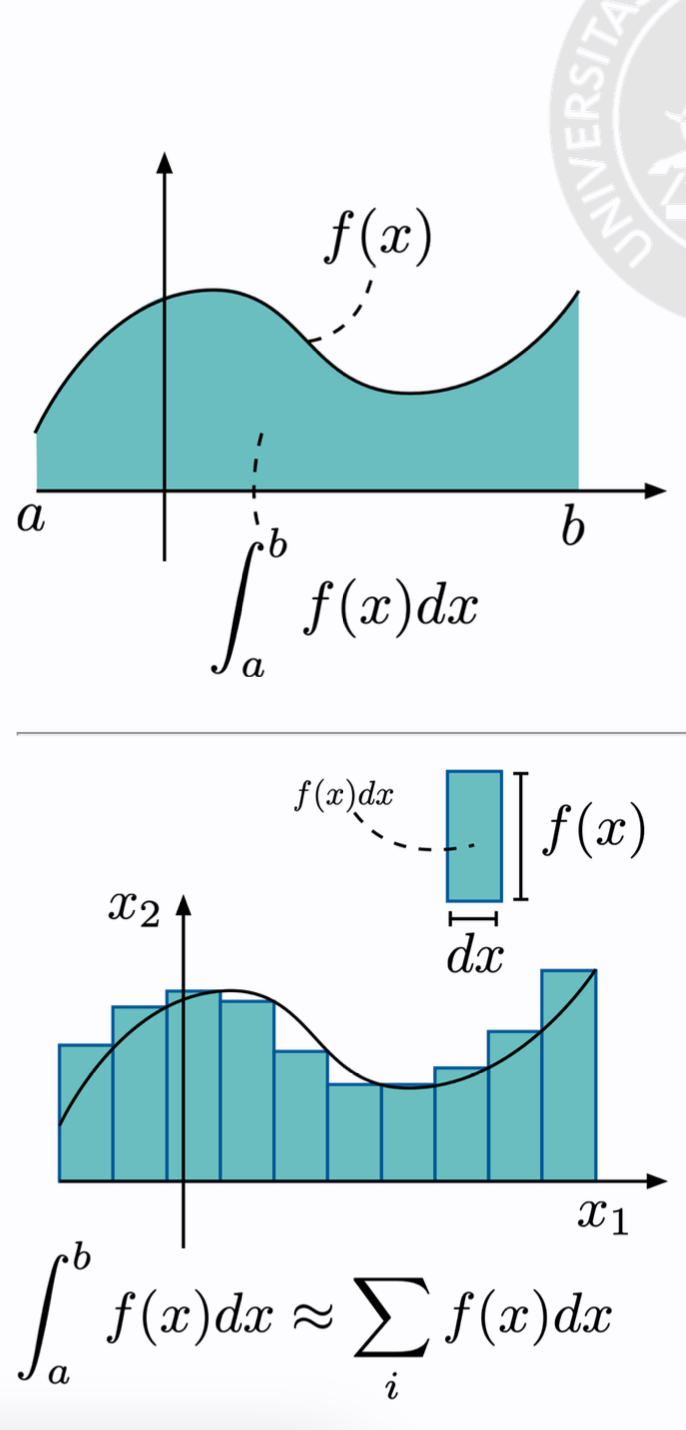
\includegraphics[scale=0.5]{images/prerequisites/integrals.png}
    \centering
\end{figure}
Ciò che è interessante è che esiste un teorema, il \textbf{teorema fondamentale dell'analisi}, che afferma che \textbf{esiste una relazione stretta tra integrali e derivate}. In particolare, se $f$ ammette un'\textbf{antiderivata} $F$, se esiste $F$ tale che $F'(x)=f(x)$ allora:
\begin{equation}
    \int f(x)dx = F(x)+C
\end{equation}
e
\begin{equation}
    \int_a^b f(x)dx = F(x)|_a^b = F(b)-F(a)
\end{equation}

\textbf{N.B.}
\begin{itemize}
    \item gli \textbf{integrali indefiniti} sono quelli per cui \textbf{non è specificato l'intervallo di integrazione} e per cui la soluzione, per convenzione, è l'antiderivata $F$;
    \item gli \textbf{integrali definiti} sono quelli per cui \textbf{è specificato l'intervallo di integrazione}.
\end{itemize}
\newpage
\textbf{Proprietà importanti degli integrali}:
\begin{itemize}
    \item \textbf{linearity} $\int \alpha f(x)+\beta g(x)dx = \alpha \int f(x)dx+\beta \int g(x)dx$
    \item \textbf{constant rule} $\int kdx = kx+C$
    \item \textbf{power rule} $\int x^n dx = \frac{x^{n+1}}{n+1}+C, n \neq-1$
    \item \textbf{log rule} $\int \frac{1}{x}dx = \ln(|x|)+C$
    \item \textbf{exponential rule} $\int a^{kx}dx = \frac{a^{kx}}{k\ln a}+C,x\neq 0$
    \item \textbf{sin rule} $\int \sin(x)dx = -\cos(x)+C$
    \item \textbf{cosin rule} $\int \cos(x)dx = \sin(x)+C$
\end{itemize}

\subsection{Derivate parziali e Gradienti}
Sia data la \textbf{funzione multivariata} $y=f(x_1,\dots,x_n)=f(x)$, dove $y\in \mathbb{R}$,$x\in \mathbb{R}^n$.


La \textbf{derivata parziale} $\frac{\delta}{\delta x_j}f(x)$ \textbf{misura come $f$ varia al variare della sola variabile $x_j$}, tutte le altre rimangono invariate:
\begin{equation}
    \frac{\delta}{\delta x_j}f(x) = \lim_{h \rightarrow 0}\frac{f(x+h\hat{i}_j)-f(x)}{h} = \lim_{h \rightarrow 0}\frac{f(x_1,\dots,x_j+h,\dots,x_n)-f(x_1,\dots,x_n)}{h}
\end{equation}
\begin{figure}[!h]
    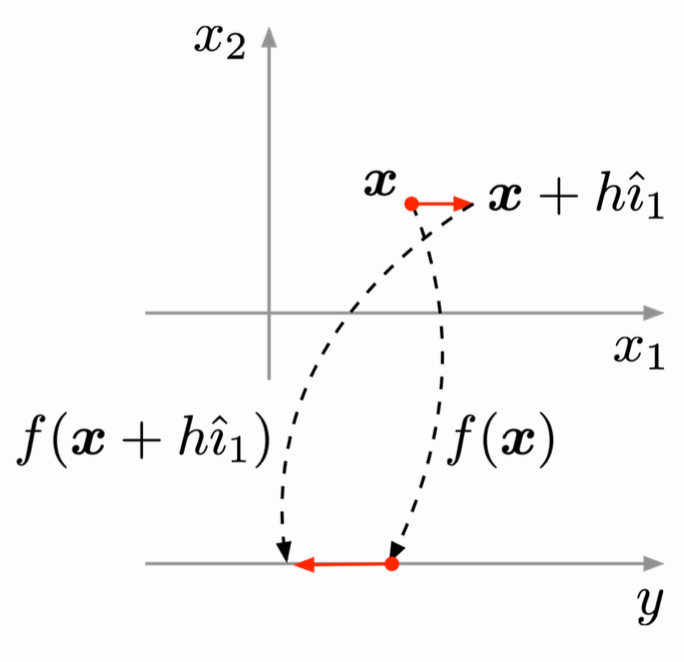
\includegraphics[scale=0.5]{images/prerequisites/partDerivatives.png}
    \centering
\end{figure}
\newline
Il \textbf{gradiente} di $f$, denotato con $\nabla_xf$ (o più semplicemente $\nabla f$) è \textbf{il vettore che contiene tutte le derivate parziali della funzione $f$}:
\begin{equation}
    \nabla f=\left[\frac{\delta f}{\delta x_1},\dots,\frac{\delta f}{\delta x_n}\right]^T.
\end{equation}
Il gradiente è un vettore con una proprietà molto particolare, per parlare della quale bisogna introdurre prima un concetto: \textbf{la regola della catena per il calcolo multivariato}.


Assumiamo $z=f(x,y)$ e siano $x,y$ variabili dipendenti da una variabile addizionale $t$ (gli input di $f$ sono a loro volta funzioni della variabile $t$, cioè abbiamo $f(x(t),y(t))$), quindi:
\begin{equation}
    \frac{dz}{dt}=\frac{\delta z}{\delta x}\frac{dz}{dt}+\frac{\delta z}{\delta y}\frac{dy}{dt}.
\end{equation}
Quello appena visto vale per 2 variabili, più in generale per $f:\mathbb{R}^n\rightarrow \mathbb{R}$, quando $x_1,\dots,x_n$ dipendono da una variabile $t$:
\begin{equation}
    \frac{df}{dt}=\sum^n_{i=1}\frac{\delta f}{\delta x_i}\frac{dx_i}{dt}.
\end{equation}
\newpage
Facciamo un esempio, date:

\begin{itemize}
    \item $(x,y)=(t^2,t)$, perciò $x(t)=t^2$ e $y(t)=t$;
    \item $z=f(x,y)=x^2y^2$
\end{itemize}
calcolare le derivata di $z$ rispetto a $t$. 
Cioè:
\begin{equation}
    \frac{\delta z}{\delta t}=\frac{\delta z}{\delta x}\frac{dx}{dt}+\frac{\delta z}{\delta y}\frac{dy}{dt}=2xy^2\cdot 2t+2x^2\cdot1=4t^5+2t^5=6t^5.
\end{equation}

\subsection{Derivate direzionali}
Vediamo ora un'applicazione immediata della regola della catena nel caso multivariato. Fino ad ora abbiamo calcolato la derivata soltanto lungo gli assi ma cosa succede se invece scegliamo di calcolarla lungo un vettore qualsiasi? Qual è il tasso di variazione della funzione rispetto al movimento in una direzione data da un vettore?


Sia $u$ un vettore unità. La derivata direzionale di $f$ nel punto $x$ nella direzione di $u$ è esattamente il \textbf{tasso di cambiamento nella direzione indicata dal vettore $u$}.
\begin{equation}
    D_uf(x)=\lim_{h\rightarrow 0}\frac{f(x+hu)-f(x)}{h}
\end{equation}
\begin{figure}[!h]
    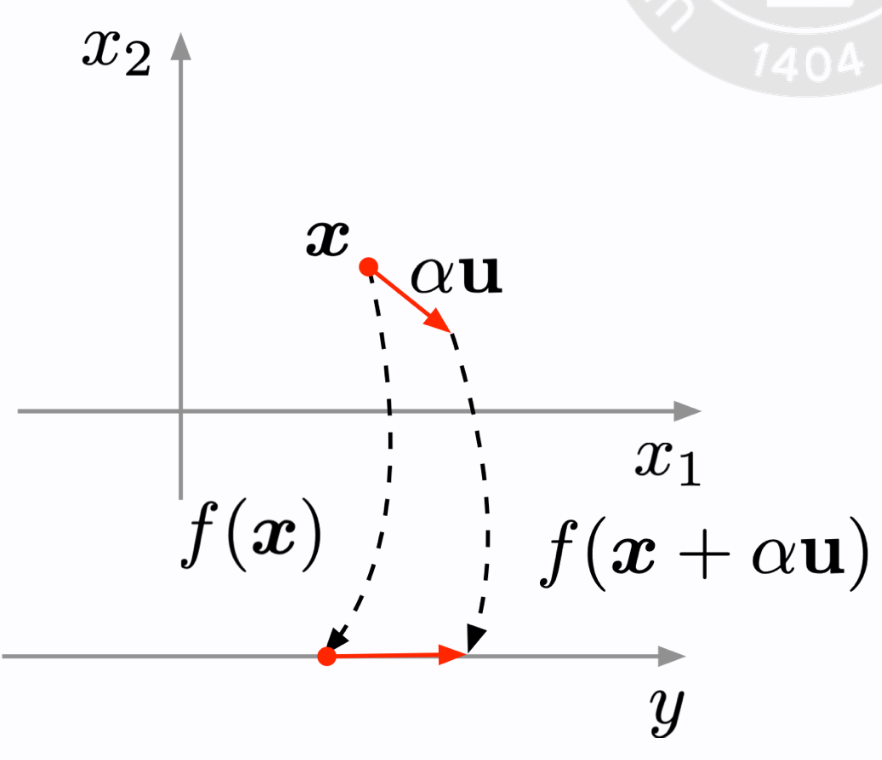
\includegraphics[scale=0.5]{images/prerequisites/dirDerivatives.png}
    \centering
\end{figure}



In altre parole, la derivata direzionale è la derivata di $f(x+\alpha u)$ rispetto ad $\alpha$ calcolata quando $\alpha = 0$.


Utilizzando la \textbf{chain rule}, possiamo facilmente calcolare un'espressione per $D_uf(x)$:
\begin{equation}
    D_uf(x)=\frac{d}{d\alpha}(x+\alpha u)\Big|_{\alpha=0}=\sum^n_{i=1}\frac{\partial f(x+\alpha u)}{\partial x_i}\Big|_{\alpha = 0}\frac{dx_i}{d\alpha}=\nabla f(x)\cdot u = u^T\nabla f(x).
\end{equation}

\newpage
Ci interessa ora \textbf{trovare la direzione nella quale la funzione cresce maggiormente}, ovvero trovare $u$ tale che $D_uf$ è maggiore. Vogliamo risolvere:
\begin{equation}
    \max_{u,u^Tu=1}D_uf(x)=\max_{u,u^Tu=1}u^T\nabla f(x)=\max_{u,u^Tu=1}|u||\nabla f(x)|cos(\theta).
\end{equation}
\begin{figure}[!h]
    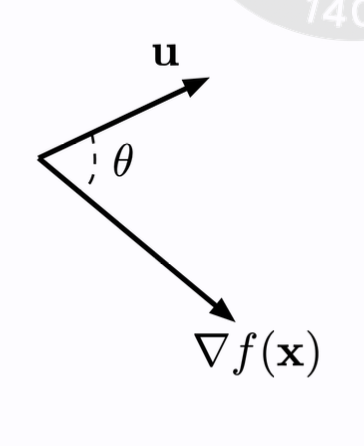
\includegraphics[scale=1]{images/prerequisites/maxGradient.png}
    \centering
\end{figure}



Ora, visto che $|u|=1$ e $\nabla f(x)$ non dipende da $u$, ciò che ci rimane è cercare $u$ tale che massimizzi il $cos(\theta)$. Questo implica però che \textbf{il massimo viene raggiunto quando $u$ ha la stessa direzione di $\nabla f(x)$}.
\newline

\textbf{IMPORTANTE: il gradiente punta nella direzione nella quale $f$ cresce di più}.
\newpage

\subsection{Matrice Jacobiana}
Quando abbiamo una funzione che oltre ad essere multivariata \textbf{ha anche molti output diversi}:
\begin{equation}
    f:\mathbb{R}^n\rightarrow \mathbb{R}^m, f(x)=[f(x)_1,\dots,f(x)_m]^T
\end{equation}
se calcoliamo tutte le derivate di un oggetto di questo tipo, stiamo calcolando lo \textbf{Jacobiano della funzione $f$}. Più formalmente essa è la matrice $J\in \mathbb{R}^n\rightarrow \mathbb{R}^m$ che contiene tutte le derivate parziali di $f(x_i),(1\leq i \leq m)$ per tutte le variabili $x_j,(1\leq j \leq n)$:
\begin{equation}
    J_{i,j}=\frac{\partial}{\partial x_j}f(x)_i
\end{equation}
o, equivalentemente, lo Jacobiano è la matrice contenente $\nabla[f(x)_i]$ nella riga $i-esima$:
\begin{equation}
    J=[\nabla[f(x)_i]^T]^m_{i=1}.
\end{equation}

\subsection{Derivate seconde}
La \textbf{derivata seconda} è la derivata di una derivata. Per esempio, sia $\mathbb{R}^n\rightarrow \mathbb{R}$, possiamo calcolare $n^2$ derivate seconde:
\begin{equation}
    \frac{\partial^2}{\partial x_i\partial x_j}f(x).
\end{equation}
La derivata seconda ci dice \textbf{come cambia la derivata prima al variare dell'input}. Può anche essere vista come una \textbf{misura della curvatura}.
\begin{figure}[!h]
    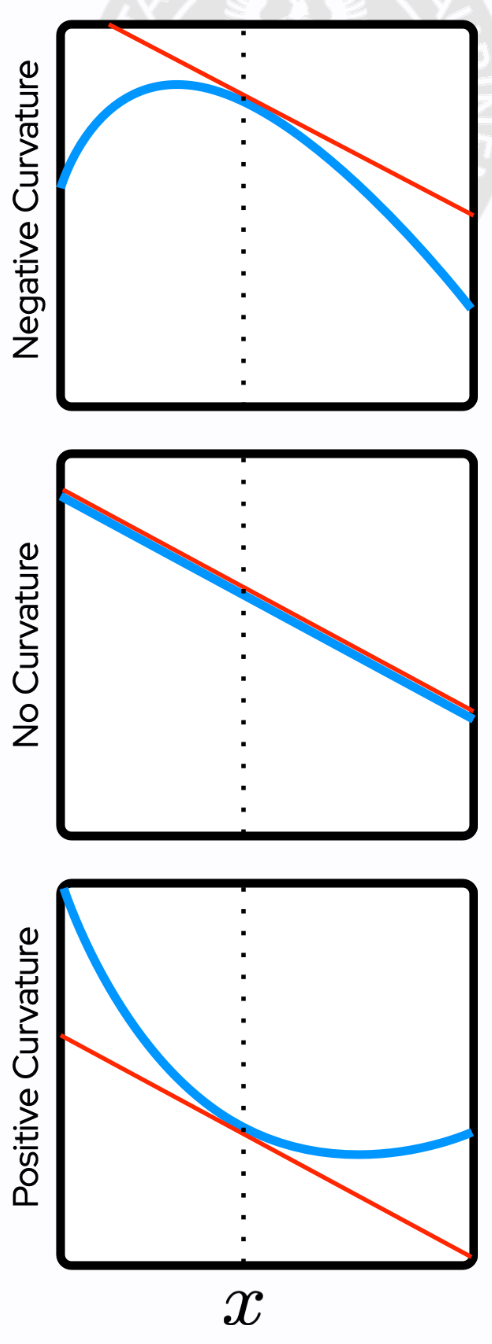
\includegraphics[scale=.55]{images/prerequisites/secondDerivative.png}
    \centering
\end{figure}


La matrice contenente tutte queste derivate parziali è chiamata \textbf{Hessiana} della funzione $f$.
\newline
\textbf{N.B.: }$H(f)=J(\nabla f)$.
\newpage

\paragraph{Proprietà della matrice Hessiana.}
\begin{itemize}
    \item in tutti in punti in cui le derivate seconde sono continue, gli operatori differenziali sono commutativi, cioè il loro ordine può essere scambiato:
        \begin{equation}
            \frac{\partial^2}{\partial x_i \partial x_j}f(x)=\frac{\partial^2}{\partial x_j \partial x_i}f(x)
        \end{equation}
        il che implica che \textbf{in quei punti la matrice Hessiana è simmetrica}.
    \item in maniera intuitiva, possiamo dire che, come la derivata seconda ci aiuta a capire se siamo in un punto di minimo o di massimo (indica la curvatura, quindi se la curvatura è verso l'alto siamo in un minimo, se è verso il basso siamo in un massimo), anche l'hessiano ci aiuta in questo senso. In particolare ci da questa informazione nel caso di \textbf{una funzione multi variata}. 


    In particolare, quando abbiamo che $\nabla f(x_0)=0$, \textbf{l'hessiano ci aiuta a capire se siamo in un minimo} (hessiano definito positivo\footnote{una matrice si definisce \textbf{positiva} quando $\forall z:z^TMz>0$}.) o \textbf{in un massimo} (hessiano definito negativo). Se l'hessiano non è ne definito positivo ne definito negativo (abbiamo almeno un autovalore che vale $0$):
    \begin{itemize}
        \item \textbf{siamo in un punto di sella}, se c'è almeno $1$ autovalore positivo e $1$ autovalore negativo;
        \item \textbf{il test non è conclusivo}, altrimenti.
    \end{itemize}
\end{itemize}
\newpage
\section{Probabilità}
La \textbf{probabilità} può essere vista come un'estensione della logica che tratta l'incertezza.


La \textbf{logica} fornisce una serie di regole formali per determinare quali proposizioni devono essere vere e quali false, data l'assunzione che un'altro set di proposizioni siano vere o false.


La \textbf{teoria delle probabilità} fornisce invece una serie di regole formali per determinare la \textbf{likelihood} di una proposizione data la likelihood di altre proposizioni.

Una \textbf{variabile casuale} è una variabile che può assumere randomicamente diversi valori. Possono essere \textbf{discrete} o \textbf{continue}.


Notazione:
\begin{itemize}
    \item variabili casuali sono indicate da lettere minuscole semplici come $x,t,\dots$;
    \item i valori assunti dalle variabili sono indicati da lettere minuscole in corsivo come $\textit{x},\textit{y},\dots$;
    \item il set di tutti i possibili valori assunti dalla variabile casuale $x$ è denotato da $\Omega_x$;
    \item a volte scriveremo $\textit{x}\in x$ per indicare $\textit{x}\in \Omega_x$;
    \item per valori che riguardano vettori e loro valori usere il grassetto quindi $\textbf{x,y}$ e $\textbf{\textit{x,y}}$.
\end{itemize}


\paragraph{Distribuzione di probabilità (Caso discreto)}
Sia data una \textbf{variabile discreta} $x={x_1,\dots,x_n}$. La \textbf{distribuzione di probabilità di una variabile discreta può essere indicata usando la probability mass function (PMF}. Normalmente essa è indicata con $\textit{P(x)}$.


La PMF \textbf{è un mapping che assegna ad ogni valore che può assumere la variabile casuale una probabilità}.
\begin{figure}[!h]
    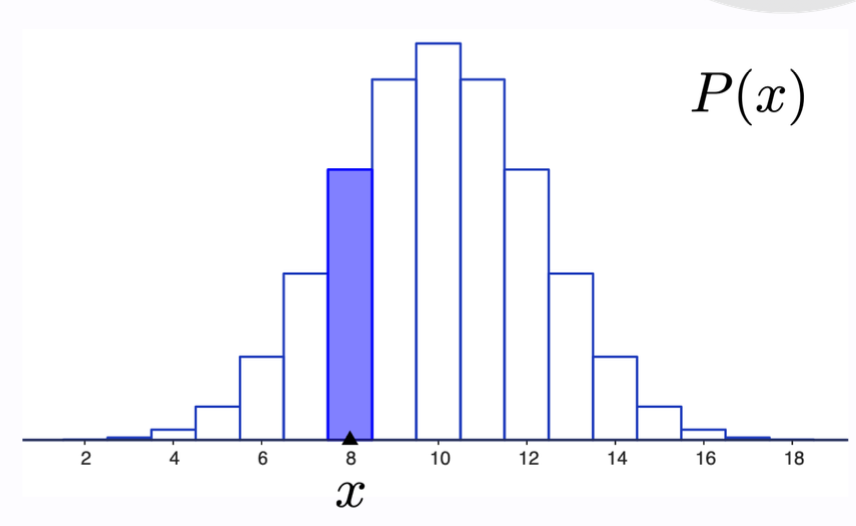
\includegraphics[scale=.5]{images/prerequisites/pmf.png}
    \centering
\end{figure}


\textbf{Notazione:} la probabilità che $\textit{P}(x=\textit{x})$ è denotata normalmente come $\textit{P}(x)$. La notazione $x\sim \textit{P}(x)$ è utilizzata per indicare che la variabile casuale $x$ segue la distribuzione descritta da $\textit{P}(x)$.



\textbf{Proprietà di una PMF:}
\begin{itemize}
    \item il dominio di $\textit{P}$ deve essere l'insieme di tutti i possibili stati di $x$;
    \item $\forall \textit{x}\in x:0\leq \textit{P}(\textit{x})\leq 1$;
    \item $\sum_{\textit{x}\in x}\textit{P}(\textit{x})=1$.
\end{itemize}
Altre proprietà utili sono:
\begin{itemize}
    \item $\textit{P}(\textit{S})=\sum_{\textit{x}\in \textit{S}}\textit{P}(\textit{x})$;
    \item $\textit{P}(\textit{$S_1$}\bigcup \textit{$S_2$})=\textit{P}(\textit{$S_1$})+\textit{P}(\textit{$S_2$})-\textit{P}(\textit{$S_1$}\bigcap \textit{$S_2$})$;
    \item $\textit{P}(\Omega \backslash \textit{S})=1-\textit{P}(\textit{S})$
\end{itemize}
con \textit{S},\textit{$S_1$},\textit{$S_2$} insiemi di possibili output; \textit{P}(\textit{S}) è una shortcut per $\textit{P}(x\in \textit{S})$ e $\Omega$ è l'insieme di tutti i possibili valori.


\paragraph{Distribuzione di probabilità (Caso continuo)}
In questo caso utilizziamo variabili \textbf{continue} e la distribuzion di probabilità non è più descrita dalla PMF ma dalla \textbf{probability density function (PDF)}.
\begin{figure}[!h]
    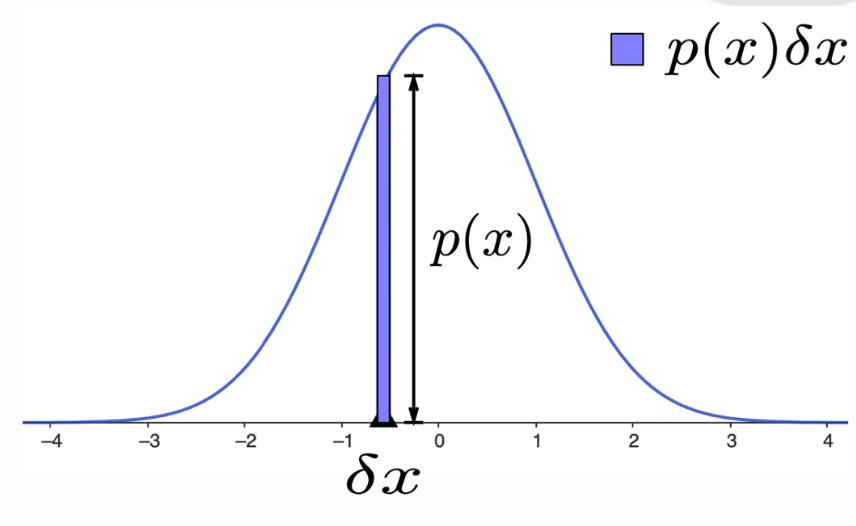
\includegraphics[scale=.5]{images/prerequisites/pdf.png}
    \centering
\end{figure}


La PDF è indicata con \textit{p} e deve soddisfare le seguenti proprietà:
\begin{itemize}
    \item il dominio di \textit{p} deve essere l'insieme di tutti i possibili stati di $\textbf{x}$;
    \item $\forall \textit{x}\in \textbf{x}:\textit{p}(\textit{x})\geq 0$, \textbf{notare che non richiediamo} $\textit{p}(\textit{x})\leq 1$;
    \item $\int \textit{p}(\textit{x})\textit{dx}=1$.
\end{itemize}

\subsection{Probabilità marginale}
A volte si conosce la distrivuzione di probabilità di un insieme di varibaili ma a noi interessa sapere la distribuzione di probabilità di un sottoineime di esse. In questo caso la distribuzione di probabilità è detta \textbf{distrubuzione marginale} di probabilità. 



Le probabilità marginali sono calcolate sommando tutti i valori delle variabili.


Per esempio, immaginiamo di avere 2 variabili casiali discrete $x$ e $y$ con una distribuzione congiunta $\textit{P}(x,y)$. La \textbf{distribuzione marginale} $\textit{P}(x)$ sarebbe:
\begin{equation}
    \forall \textit{x}\in x \textit{P}(\textit{x})=\sum_y\textit{P}(x=\textit{x},y=\textit{y});
\end{equation}
per le varabili continue:
\begin{equation}
    \textit{p}(\textit{x})=\int \textit{p}(\textit{x,y})\textit{dy}.
\end{equation}
\begin{figure}[!h]
    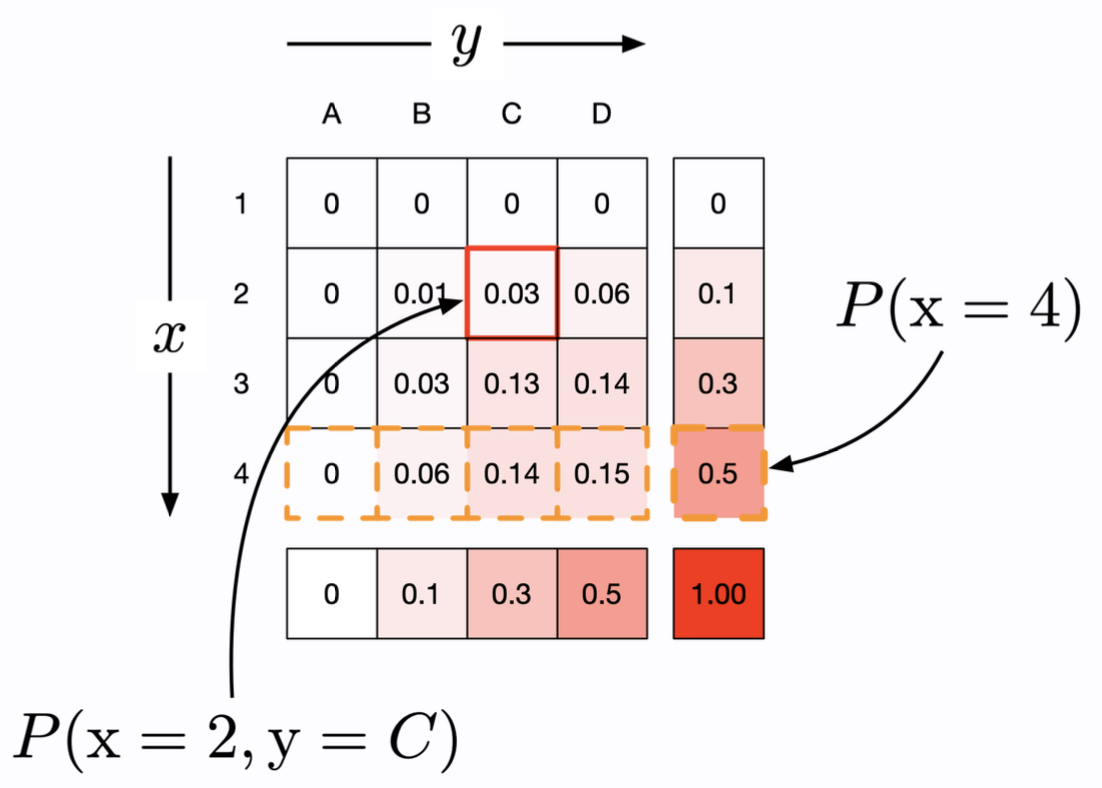
\includegraphics[scale=.5]{images/prerequisites/margProbability.png}
    \centering
\end{figure}
\newpage
\subsection{Probabilità condizionta}
In molti casi, siamo interessati alla probabilità di un evento dato un altro evento accaduto. Questa è la \textbf{probabilità condizionata}. La probabilità condizionata che $y=\textit{y}$ dato $x\textit{x}$ è indicata come
\begin{equation}
    \textit{P}(\text{y}=y|\text{x}=x).
\end{equation}
Può essere calcolata con la formula:
\begin{equation}
    P(\text{y}=y|\text{x}=x)=\frac{P(\text{y}=y,\text{x}=x)}{P(\text{x}=x)}.
\end{equation}
\begin{figure}[!h]
    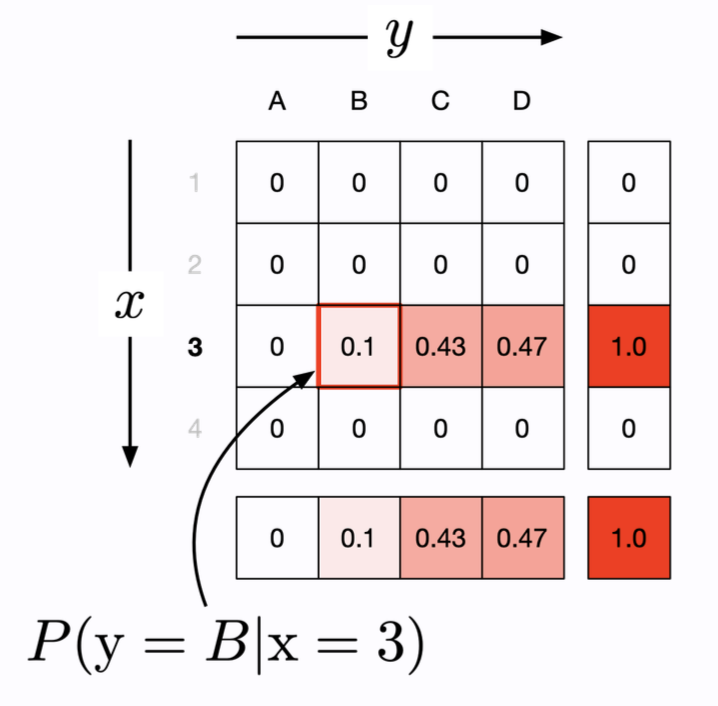
\includegraphics[scale=.5]{images/prerequisites/condProb.png}
    \centering
\end{figure}



La cosa interessante da notare è che questa \textbf{è una distrubizione completamente nuova su y}.


\subsection{Chain rule della probabilità condizionata}
Qualsiasi distribuzione di probabilità congiunta su più variabili casuali può essere decomposta in prodotti di distrivuzioni condizioni di una sola variabile:
\begin{equation}
    P(\text{x}^{(1)},\dots,\text{x}^{(n)})=P(\text{x}^{(1)})\prod^n_{i=2}P(\text{x}^{(i)}|\text{x}^{(1)},\dots,\text{x}^{(i-1)}).
\end{equation}
\textbf{Esempi}:
\begin{itemize}
    \item $P(\text{a}|\text{b,c})=\frac{P(\text{a,b,c})}{P(\text{b,c})} \Rightarrow P(\text{a,b,c})=P(\text{a$|$b,c})P(\text{b,c})$;
    \item similmente avremo che $P(\text{b,c})=P(\text{b$|$c})P(\text{c})$.
\end{itemize}
\subsection{Indipendenza}
Due variabili casuali x e y sono \textbf{indipendenti} (indicate con x$\perp$y) se \textbf{la loro distribuzione di probabilità può essere espressa come prodotto delle loro probabilità marginali}:
\begin{equation}
    \forall x\in \text{x},y\in \text{y}:p(\text{x}=x,\text{y}=y)=p(\text{x}=x)p(\text{y}=y).
\end{equation}
\textbf{Nota:}
\begin{equation}
    \text{x}\perp\text{y}\Longleftrightarrow \forall x\in \text{x},y\in \text{y}:p(x|y)=p(x) \wedge p(y|x)=p(y).
\end{equation}
Se è vero che le due variabili sono indipendenti valgono anche che:
\begin{itemize}
    \item $P(x|y)=P(x)$;
    \item $P(y|x)=P(y)$
\end{itemize}
il che è abbastanza intutivo, se le due variabili sono indipendenti le loro probabilità non hanno nessun impatto l'una sull'altra.
Inoltre, due variabili casuali x e y sono \textbf{condizionatamente indipenti} data una variabile casuale z (scriveremo x$\perp$y|z) se la distribuzione di probabilità condizionale su x e y fattorizza in questo modo per ogni valore di z:
\begin{equation}
    \forall x\in \text{x},y\in \text{y,z}\in \text{z}:p(\text{x}=x,\text{y}=y|\text{z}=z)=p(\text{x}=x|\text{z}=z)p(\text{y}=y|\text{z}=z).
\end{equation}

\subsection{Expectation (Valore atteso)}
Il \textbf{valore atteso} (spesso denotato da $\mu$) di una funzione $f(x)$ rispetto alla distribuzione di probabilità $P(\text{x})$ è la media o il valore medio che $f$ assume quando $x$ è tratto da $P$.



\textbf{Variabili discrete:}
\begin{equation}
    \mathbb{E}_{\text{x}\sim P}[f(x)]=\sum_xP(x)f(x).
\end{equation}
\textbf{Variabili continue:}
\begin{equation}
    \mathbb{E}_{\text{x}\sim p}[f(x)]=\int p(x)f(x)dx.
\end{equation}
\textbf{Nota:} il valore atteso è un \textbf{operatore lineare}:
\begin{equation}
    \mathbb{E}[\alpha f(x)+\beta g(x)]=\alpha \mathbb{E}[f(x)] + \beta \mathbb{E}[g(x)].
\end{equation}

\subsection{Varianza e Deviazione standard}
\paragraph{Varianza}
La varianza (spesso denotata con $\sigma^2$) restituisce la misure di \textbf{quando i valori di una funzione di una variabile casuale x variano rispetto al campionamento di diversi valori di x dalla sua distribuzione di probabilità}:
\begin{equation}
    \text{Var}[f(x)]=\mathbb{E}[(f(x)-\mathbb{E}[f(x)])^2].
\end{equation}
\textbf{Esempio:}
La varianza può anche essere calcolata come $\text{Var}[f(x)]=\mathbb{E}[f(x)^2]-\mathbb{E}[f(x)]^2$:
\begin{gather}
    \text{Var}[f(x)]=\mathbb{E}[(f(x)-\mathbb{E}[f(x)])^2]\\
    =\mathbb{E}[(f(x)^2-2f(x)\mathbb{E}[f(x)])+\mathbb{E}[f(x)])^2]\\
    =\mathbb{E}[f(x)^2]-2\mathbb{E}[f(x)\mathbb{E}[f(x)]])+\mathbb{E}[\mathbb{E}[f(x)]^2]\\
    =\mathbb{E}[f(x)^2]-2\mathbb{E}[f(x)]\mathbb{E}[f(x)]+\mathbb{E}[f(x)]^2\\
    =\mathbb{E}[f(x)^2]-\mathbb{E}[f(x)]^2.
    %%sistemare spaziatura
\end{gather}


\paragraph{Deviazione Standard.}
La \textbf{deviazione standard} (denotata da $\sigma$) è data dalla radice quadrata della varianza.


\textbf{Utile da sapere:} per una variabile descritta da una distribuzione normale, circa il 95\% dei punti cade in un range di $\mu \pm2\sigma$.



\paragraph{Covarianza.} La \textbf{covarianza} è una misura di quanto due variabili casuali siano relazionate l'una con l'altra:
\begin{gather}
    \text{Cov(x,y)}=\mathbb{E}_{x,y\sim P(\text{x,y})}[(x-\mathbb{E[\text{x}]})(y-\mathbb{E}[\text{y}])]\\
    =\mathbb{E}_{x,y\sim P(\text{x,y})}[(x-\mu_x)(y-\mu_y)]
\end{gather}
\begin{figure}[!h]
    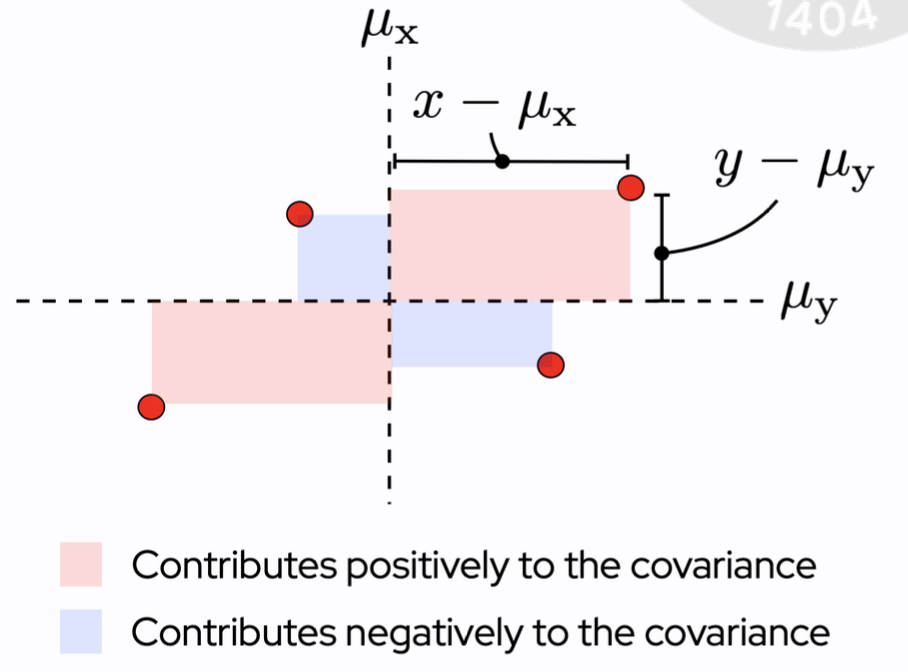
\includegraphics[scale=.5]{images/prerequisites/covariance.png}
    \centering
\end{figure}



L'idea è che, se $\mu_x$ e $\mu_y$ rappresentano gli assi (come in figura), prendendo un punto a caso (per esempio (x,y), punto rosso in alto a destra) mi posso chiedere in che maniera contribuisca al calcolo della covarianza. La risposta è che il contributo corrisponde all'area (rossa, nel caso di (x,y)) che sta sotto il rettangolo di cui il nostro punto rappresenta uno dei vertici. Quest'area contribuisce positivamente al calcolo se (x,y) sono entrambe maggiori delle rispettive medie, negativamente altrimenti.



\textbf{Nota:} la covarianza \textbf{è affetta dalla scala delle variabili}.



\paragraph{Correlazione.} La \textbf{correlation} risolve esattamente il problema appena descritto, cioè il fatto che la covarianza sia affetta dalla scala. Essa garantisce che la relazione tra le variabili sia misurata senza che sia influenzata dalle loro magnitudini invividuali:
\begin{equation}
    \text{Corr}(x,y)=\frac{\text{Cov}(x,y)}{\sigma_x\sigma_y}.
\end{equation}
Il risultato di questa formula restituisce un numero compreso in $[-1,1]$ ($+1$ le varabili assumono sempre gli stessi valori, $-1$ le variabili assumono sempre valori opposti) e una correlazione vicina a $\pm1$ indica una relazione forte tra le variavili mentre una correlazione vicina alle $0$ indica che le varibaili \textbf{potrebbero essere indipendenti}. 


\paragraph{Covarianza vs Dipendenza.} Le nozioni di \textbf{covarianza} e \textbf{dipendenza} sono correlate ma \textbf{sono concetti distinti}. Infatti:
\begin{itemize}
    \item due variabili che sono indipendenti hanno zero covarianza;
    %prima o poi scrivo questa dimostrazione, minuti 50 della lezione sulle probabilità

    
    \item due variabili che hanno covarianza diversa da zero sono dipendenti;
    \item due variabili possono avere covarianza pari a zero ed essere comunque dipendenti (come mostrato nella figura).
\end{itemize}
\begin{figure}[!h]
    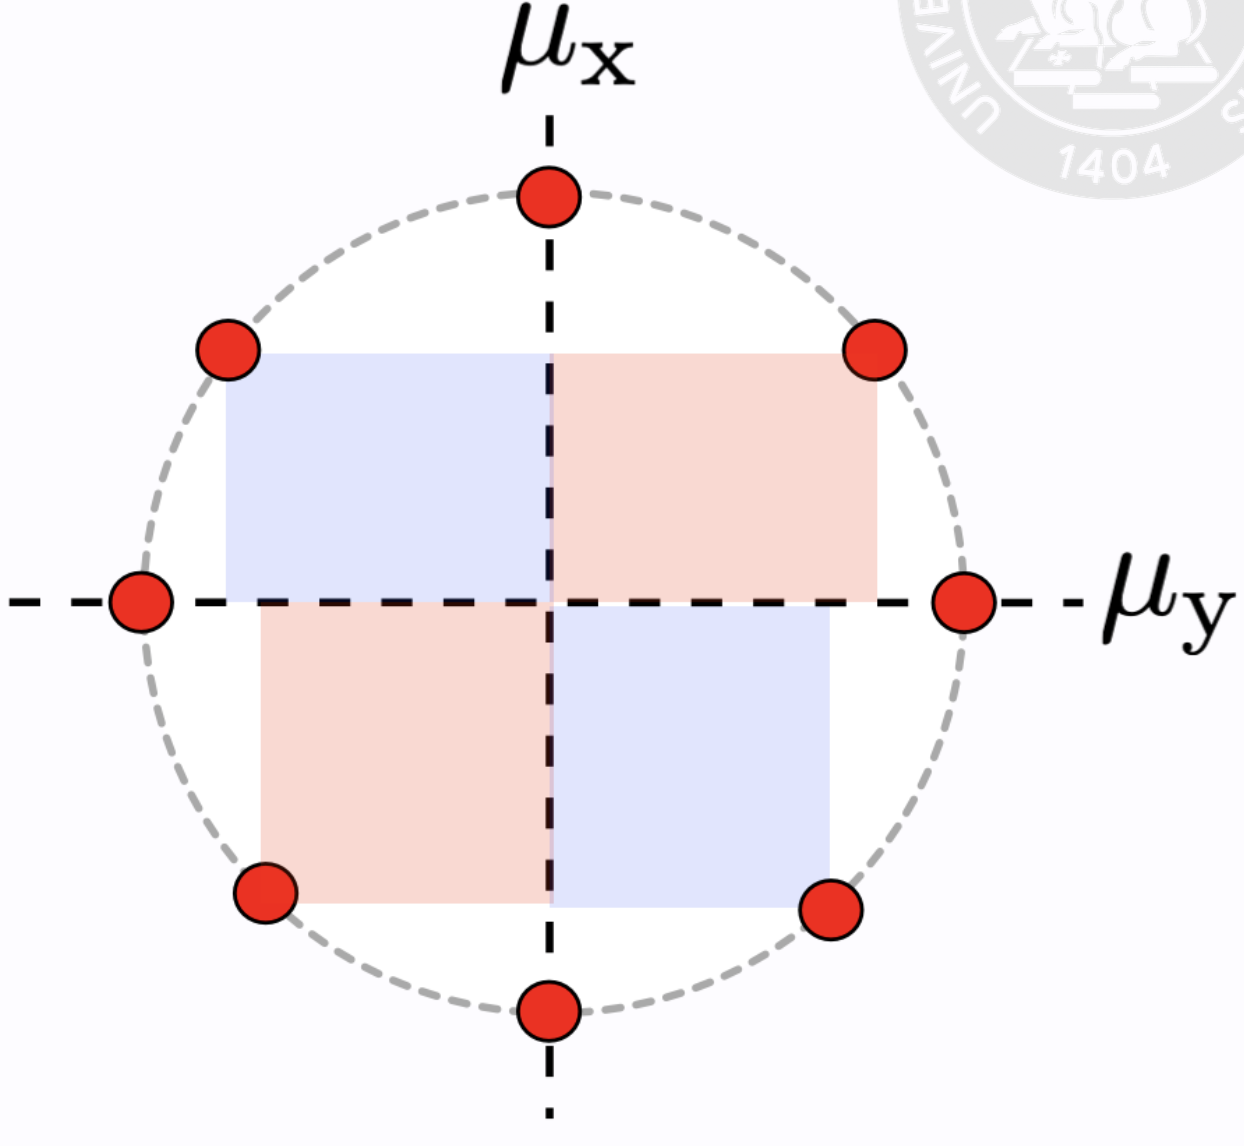
\includegraphics[scale=.25]{images/prerequisites/covVSdep.png}
    \centering
\end{figure}
\newpage

\subsection{Distribuzioni di Probabilità Comuni}
\paragraph{Bernoulli distribution.} Si tratta di una distribuzione di una singola variabile casuale \textbf{binaria} (semplicemente la distribuzione che modella il lancio di una moneta). E' controllata da un singolo parametro $\phi\in[0,1]$, il quale restituisce la probabilità che la variabile casuale abbia valore uguale ad $1$. Ha le seguenti proprietà:
\begin{itemize}
    \item $P(\text{x}=1)=\phi$;
    \item $P(\text{x}=0)=1-\phi$;
    \item $P(\text{x}=x)=\phi^x(1-\phi)^{1-x}$;
    \item $\mathbb{E}=\phi$;
    \item Var$(x)=\phi(1-\phi)$.
\end{itemize}


\paragraph{Multinoulli distribution.} E' un'estensione della distribuzione di Bernoulli a più di un risultato. La distribuzione \textbf{multinormale} o \textbf{categorica} tratta una singola variabile discreta com $k$ differenti stati, dove $k$ è finito.


E' parametizzata da un vettore \textbf{p}$\in[0,1]^k$, con \textbf{1}$^T$\textbf{p}$=1$ (che indica che gli elementi del vettore $p$ devono sommare ad $1$) dove $p_i$ restituisce la probabilità dell'$i-$esimo stato. 


Questo tipo di distribuzione è spesso usata per descrivere valori categorici, quindi normalmente non assumiamo che lo stato 1 ha valore numerico 1. Per questa ragione, \textbf{normalmente non abbiamo bisogno di calcolare l'expectation o la varianza} di variabili casuali di distribuzione multinormale.



\paragraph{Binomial distribution.} La distribuzione binomiale restituisce \textbf{la probabilità di osservare un dato numero di successi ripetendo l'esperimento di Bernoulli}. E' parametrizzata da:
\begin{itemize}
    \item $p$: la probabilità di successo dell'esperimento di Bernoulli;
    \item $N$: il numero totale di ripetizioni dell'esperimento di Bernoulli.
\end{itemize}
Se x$\sim$Bi($p,N$), allora:
\begin{gather}
    P(\text{x}=k)=\binom{N}{k}p^k(1-p)^{N-k}\\
    \mathbb{E}[\text{x}]=Np\\
    \text{Var[x]}=Np(1-p)
\end{gather}
\begin{figure}[!h]
    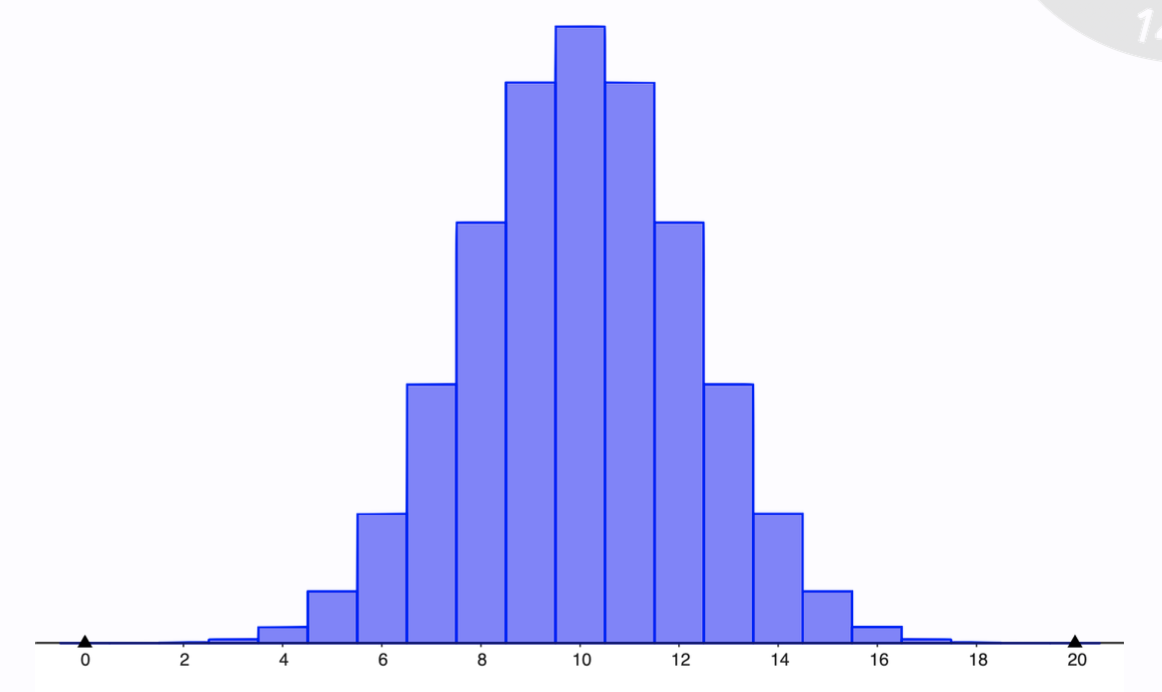
\includegraphics[scale=.5]{images/prerequisites/binomial.png}
    \centering
\end{figure}
\newpage
\paragraph{Gaussian distribution.} La distribuzione più utilizzata per i numeri reali è la \textbf{distribuzione normale}, anche detta \textbf{distribuzione Gaussiana}.


Una Gaussiana è parametrizzata da una media $\mu$ e da una varianza $\sigma^2$. Se x$\sim\mathcal{N}(\mu,\sigma^2)$, allora la PDF di x è data da:
\begin{equation}
    p(x)=\frac{1}{\sqrt{2\pi\sigma^2}}\text{exp}\Big( -\frac{(x-\mu)^2}{2\sigma^2} \Big).
\end{equation}
\begin{figure}[!h]
    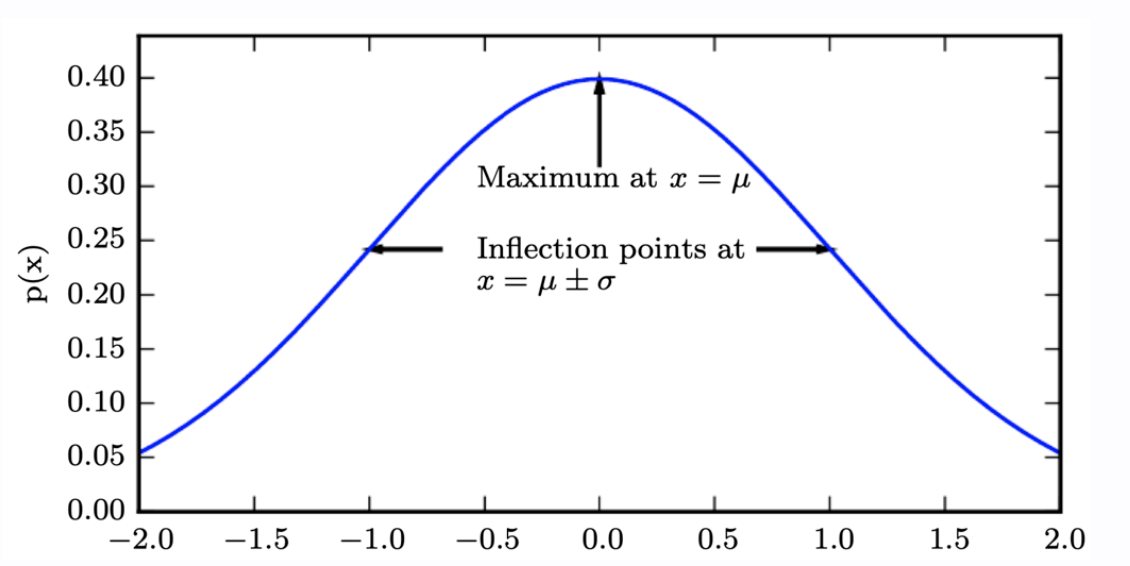
\includegraphics[scale=.5]{images/prerequisites/gaussian.png}
    \centering
\end{figure}



In realtà molte delle distribuzioni che vogliamo modellare sono molto vicine ad una distribuzione normale.
\paragraph{Teorema del limite centrale.} Sia $X_1,\dots,X_n$ una sequenza di variabili casueli indipendenti identicamente distribuite con media $\mu$ e varianza $\sigma^2$. La distribuzione della somma $S=\sum_{i=1}^nX_i$ tende ad una distribuzione normale $\mathcal{N}(n\mu,n\sigma^2)$ per $n$ che tende all'infinito. Anche la media $\frac{1}{n}S$ tende ad una distribuzione normale $\mathcal{N}(\mu,\frac{\sigma^2}{n})$ se $n$ tende all'infinito.
\newline
\newline
Tra tutte le possibili distribuzioni di probabilità con la stessa media e varianza, la distribuzione normale \textbf{codifica la massima quantità di incertezza} (cioè è la distribuzione che ha entropia massima). Ciò significa che se dobbiamo studiare un fenomeno di cui non abbiamo informazioni, l'ipotesi che si predilige, facendo meno assunzioni addizionali possibili riguardo il mondo esterno, è che segua la distribuzione normale.
\newline
\newline
La distribuzione normale si generalizza al caso multivariato $\mathbb{R}^n$:
\begin{equation}
    \mathcal{N}(\textbf{x;$\mu$,$\Sigma$)}=\frac{1}{\sqrt{(2\pi)^n\text{det}(\Sigma)}}\text{exp}\Big(-\frac{1}{2}(\textbf{x$-\mu$})^T\textbf{$\Sigma$}^{-1}(\textbf{x$-\mu$}) \Big)
\end{equation}
\begin{itemize}
    \item \textbf{$\mu$}: vettore che denota la media della distribuzione;
    \item \textbf{$\Sigma$}: la matrice di covarianza della distribuzione.
\end{itemize}
Leggiamo l'equazione:
\begin{itemize}
    \item $\frac{1}{\sqrt{(2\pi)^n\text{det}(\Sigma)}}$ è in realtà lo stesso fattore che troviamo nella Gaussiana ma che ha al posto di $\sigma^2$ il determinante della matrice di covarianza. Come nel caso precedente il fattore serve per riuscire a gestire meglio l'integrale;
    \item $(\textbf{x$-\mu$})^T\textbf{$\Sigma$}^{-1}(\textbf{x$-\mu$})$ non è altro che un'espressione quadratica, la cui formula generale è $z^TMz$.
\end{itemize}
Quindi nella sostanza è abbastanza simile alla formual della Gaussiana.
Le matrici di covarianza sono \textbf{simmetriche} e \textbf{semi-definite positive} e la loro diagonale principale contiene le varianze.


Se \textbf{$\Sigma=\sigma^2\mathbf{I}$}, la varianza è la stessa in ogni direzione: \textbf{la distribuzione è definita isotropica}.
\newpage
\paragraph{Exponential e Laplace distributions.} Nel contesto del deep learning, spesso vogliamo avere una distribuzione di probabilità con un picco in $x=0$. Per ottenere questo, possiamo usare la \textbf{distribuzione esponenziale}:
\begin{equation}
    p(x;\lambda)=\lambda\text{exp}(-\lambda x), x\geq0.
\end{equation}
\begin{figure}[!h]
    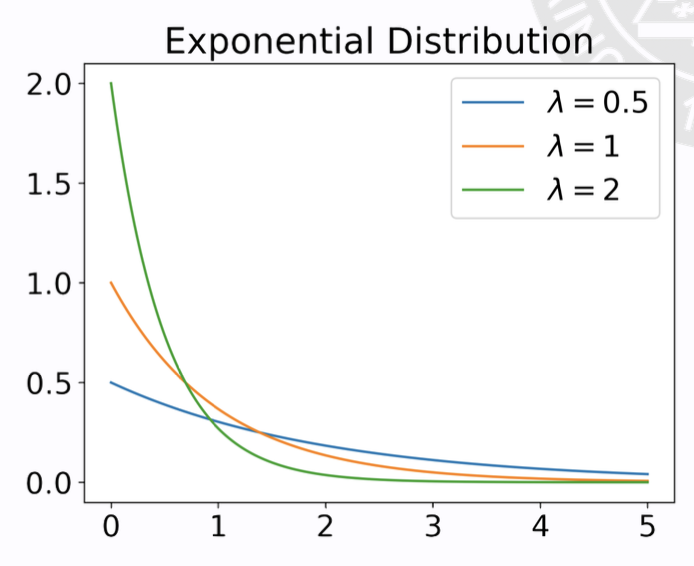
\includegraphics[scale=.7]{images/prerequisites/exp.png}
    \centering
\end{figure}
Il parametro $\lambda$ definisce quanto ripido è il picco.



Una distribuzione di probabilità correlata alla precedente, che ci permette di piazzare un picco di massa di probabilità in un punto arbitrario $\mu$ è la \textbf{distribuzione di Laplace}:
\begin{equation}
    \text{Laplace}(x;\mu,\gamma)=\frac{1}{2\gamma}\text{exp}\Big(-\frac{|x-\mu|}{\gamma} \Big)
\end{equation}
\begin{figure}[!h]
    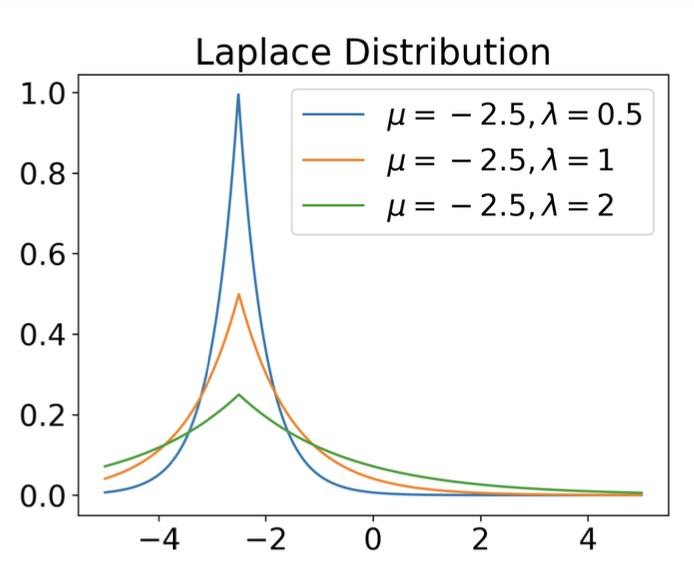
\includegraphics[scale=.7]{images/prerequisites/laplace.png}
    \centering
\end{figure}



In questo caso $\gamma$ ha lo stesso ruolo che aveva $\lambda$ nell'esponenziale mentre, come detto $\mu$ definisce in quale punto si trova il picco.
\newpage
\paragraph{Distribuzioni di tipo Mixture.} E' comune anche definire distribuzioni di probabilità a partire dalla combinazione di diverse semplici distribuzioni. Un modo comune di combinare distribuzioni è quello di costrure una \textbf{mixture distribution}:
\begin{equation}
    P(\text{x})=\sum_iP(\text{c}=i)P(\text{x|c}=i),
\end{equation}



dove $P(\text{c})$ è una distribuzione multinormale sui componenti della mistura.
\begin{figure}[!h]
    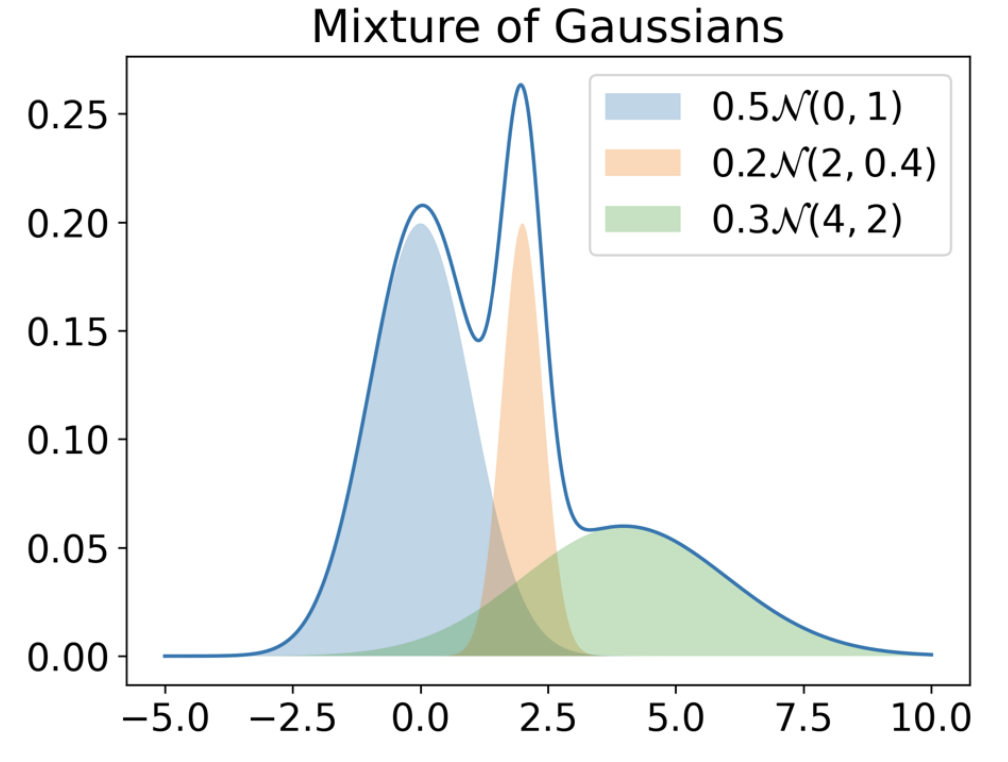
\includegraphics[scale=.6]{images/prerequisites/mixture.png}
    \centering
\end{figure}
\paragraph{Regola di Bayes.} Ci troviamo spesso in situazioni dove conosciamo $P(\text{y|x})$ e ci interessa conoscere $P(\text{x|y})$. Fortunatamente, se conosciamo anche $P(\text{x})$ e $P(\text{y})$, possiamo calcolare $P(\text{x|y})$ usando la \textbf{regola di Bayes}:
\begin{equation}
    P(\text{x$|$y})=\frac{P(\text{x})P(\text{y$|$x})}{P(\text{y})}.
\end{equation}




\paragraph{Variabili latenti.}
I mixture model ci permettono di accennare un concetto che avrà molta importanza in futuro: \textbf{le variabili latenti}.
\begin{figure}[!h]
    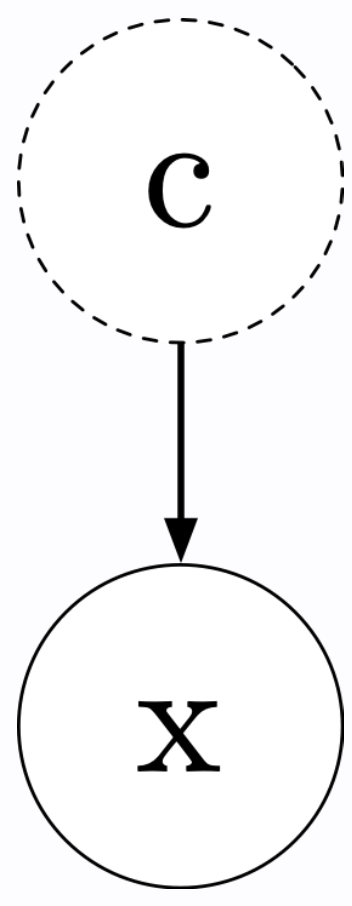
\includegraphics[scale=.3]{images/prerequisites/varLat.png}
    \centering
\end{figure}



Una variabile latente è una variabile casuale la quale \textbf{non può essere osservata direttamente} e che governa la distribuzione che stiamo osservando. Spesso assumere che ci sia una variabile latente ci permette di modellare e gestire meglio i problemi.
La variabile identità della componente \textbf{c} del mixture model ne fornisce un esempio.



Le variabili latenti potrebbero essere relazionate ad \textbf{x} attraverso la distribuzione congiunta, in questo caso, $P(\text{x,c})=P(\text{x$|$c})P(\text{c})$.
\newpage
\subsection{Proprietà utili delle funzioni comuni}
\paragraph{Sigmoid.} E' spesso usata per produrre il parametro $\phi$ della distribuzione di Bernoulli. E' denotata con $\sigma$ e definita come:
\begin{equation}
    \sigma(x)=\frac{1}{1+\exp(-x)}.
\end{equation}
\begin{figure}[!h]
    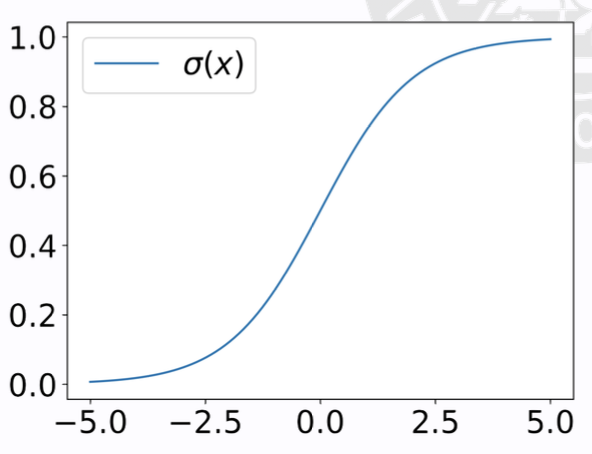
\includegraphics[scale=.7]{images/prerequisites/sigmoid.png}
    \centering
\end{figure}


\paragraph{Softplus.} Una versione \textbf{smooth} di $x^+=\max(0,x)$, è denotata con $\zeta$ e definita come:
\begin{equation}
    \zeta(x)=\log(1+\exp(x)).
\end{equation}
\begin{figure}[!h]
    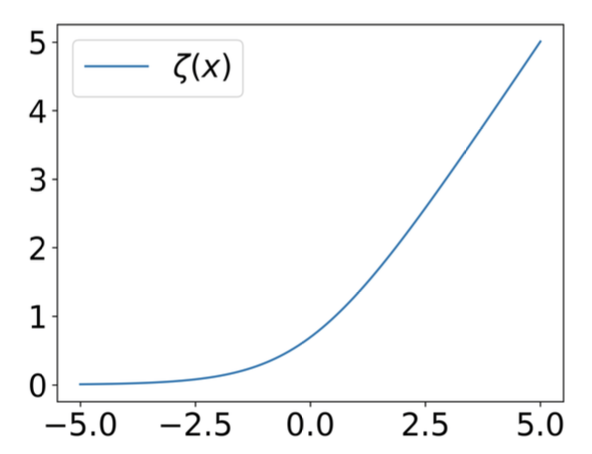
\includegraphics[scale=.7]{images/prerequisites/softplus.png}
    \centering
\end{figure}



\paragraph{Proprietà utili delle funzioni comuni.}
\begin{itemize}
    \item la sigmoide \textbf{si satura} per valori grandi (positivi e negativi) di $x$;
    \item $\sigma(x)=\frac{\exp(x)}{\exp(x)+\exp(0)}$;
    \item $\frac{d}{dx}\sigma(x)=\sigma(x)(1-\sigma(x))$;
    \item $1-\sigma(x)=\sigma(-x)$;
    \item $\log\sigma(x)=-\zeta(-x)$;
    \item $\frac{d}{dx}\zeta(x)=\sigma(x)$;
    \item $\forall x\in(0,1):\sigma^{-1}(x)=\log(\frac{x}{1-x})$;
    \item $\forall x>0:\zeta^{-1}(x)=\log(\exp(x)-1)$;
    \item $\zeta(x)=\int^x_{-\infty}\sigma(y)dy$;
    \item $\zeta(x)-\zeta(-x)=x$.
\end{itemize}
\newpage
\subsection{Measure Theory}
Una corretta comprensione formale delle variabili casuali continue e della probability density function richiede uno sviluppo della teoria delle probabilità attravero un ramo della matematica conosciuto come \textbf{measure theory} o teoria della misura.
\newline
\newline
Senza di essa, potremmo ritrovarci in situationi paradossali come:



\textit{è possibile costruire due insiemi} $S_1$ \textit{e} $S_2$, \textit{con} $S_1\cap S_2=\emptyset$ \textit{tali che} $p(x\in S_1)+p(x\in S_2)>1$.
\newline
\newline
Questi paradossi spesso riguardano la costruzione di insiemi \textit{molto esotici}, come insiemi frattali o che derivano da trasformazioni di numeri razionali, ma la possibilità esiste.
\newline
\newline
Uno dei contributi chiave di questa è il fatto che fornisca un framework per caratterizzare insiemi in cui le probabilità possono essere calcolate in maniera consistente, evitando paradossi.


La measure theory fornisce un modo rigoroso per descrivere che \textbf{un insieme di punti è trascurabilmente piccolo}. In questo caso diremo che l'insieme ha \textbf{measure zero}, o misura zero. 
\newline
\textbf{Esempio:}
\textit{Una linea in $\mathbb{R}^2$ ha measure zero}.
\newline
\newline
Qualsiasi \textbf{unione di insiemi numerabili} che abbiano measure zero ha anch'essa measure zero (quindi l'insieme di tutti i numeri razionali ha measure zero).


Quando una proprietà vale in tutto lo spazio tranne che per un punto in un insieme di misura zero, diremo che quella proprietà vale \textbf{quasi ovunque}.



\paragraph{Dettagli tecnici delle variabili continue.} Trattiamo ora le variabili casuali continue che sono \textbf{funzioni deterministici di altre variabili}. 



Supponiamo di avere due variabili casuali, \textbf{x} e \textbf{y}, tali che \textbf{$y$}=g(\textbf{$x$}), dove $g$ è una trasformazione differenziabile, invertibile e continua.


Sfortunatamente: $p_\text{y}(y)\neq p_\text{x}(g^{-1}(y))$.
\newline
\newline
Sia y$=\frac{\text{x}}{2}$ e x$\sim U(0,1)$. In questo caso abbiamo:
\begin{itemize}
    \item $y=g(x)=\frac{x}{2}$;
    \item $x=g^{-1}(y)=2y$.
\end{itemize}
\begin{figure}[!h]
    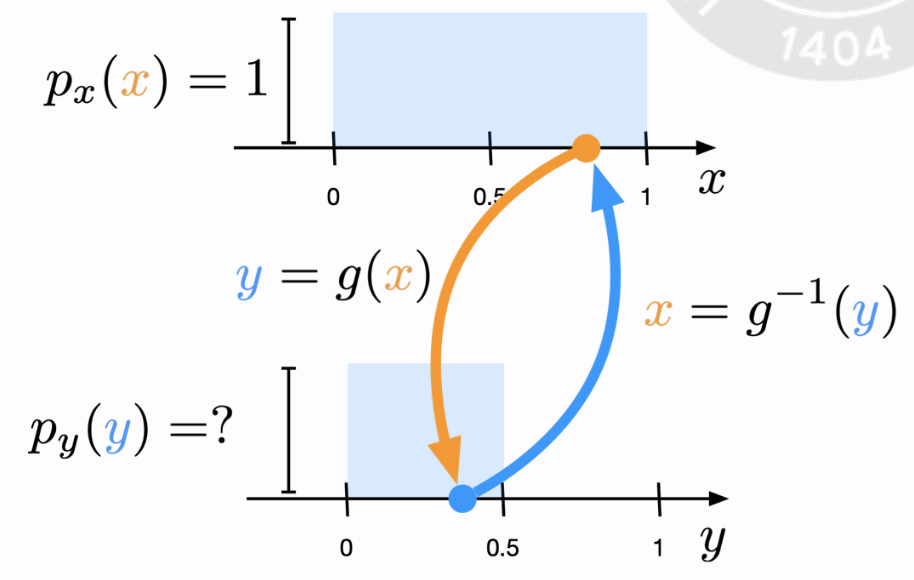
\includegraphics[scale=.5]{images/prerequisites/ex01.png}
    \centering
\end{figure}



Ci aspetteremo che $p_y(y)=p_x(2y)$, ma non è questo il caso. Infatti, se così fosse, $p_y(y)$ sarebbe uguale a zero dapperttutto ad eccezione dell'intervallo $[0,\frac{1}{2}]$ dove sarebbe $1$. Invece:
\begin{equation}
    \int_{-\infty}^\infty p_y(y)dy=\int_0^{0.5}1dy=x\Big|^{0.5}_0=0.5-0=0-5
\end{equation}


Il problema con questo approccio è che fallisce nel tenere conto della distorsione dello spazio introdotta dalla funzione $g$.



La probabilità che $x$ si trovi in una regione infinitesimamente piccola con volume $\delta x$ è data da $p(x)\delta x$.
\begin{figure}[!h]
    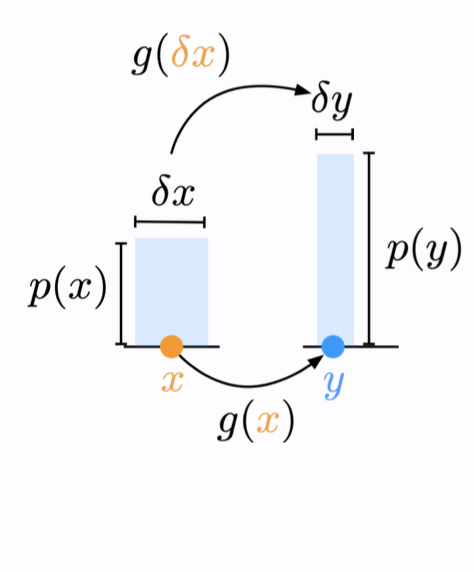
\includegraphics[scale=.7]{images/prerequisites/ex02.png}
    \centering
\end{figure}



Siccome $g$ può espandere o contrarre lo spa<io, il volume infinitesimale che circonda $x$ nello spazio $x$ potrebbe avere un volume differente nello spazio $y$.



Per correggere il problema abbiamo bisogno di preservare la proprietà:
\begin{equation}
    |p_y(g(x))dy|=|p_x(x)dx|
\end{equation}
che porta a:
\begin{equation}
    p_y(g(x))|dy|=p_x(x)|dx| \Rightarrow p_x(x)=p_y(g(x))\Big| \frac{d}{dx}g(x) \Big|
\end{equation}
o, equivalentemente:
\begin{equation}
    p_y(y)|dy|=p_x(g^{-1}(y))|dx| \Rightarrow p_y(y)=p_x(g^{-1}(y))\Big| \frac{d}{dy}g(y) \Big|.
\end{equation}



Nel nostro esempio:
\begin{equation}
    p_y(y)=p_x(g^{-1}(y))\Big| \frac{\partial g^{-1}(y)}{\partial y} \Big|=p_x(2y)\Big| \frac{d}{dy}2y\Big|=1\cdot2=2
\end{equation}
e
\begin{equation}
    \int_0^{0.5}p_y(y)dy=\int_0^{0.5}2dy=1.
\end{equation}
In \textbf{dimensioni maggiori} $g:\mathbb{R}^m\rightarrow\mathbb{R}^n$, la derivata si generalizza alla matrice jacobiana e il valore assoluto al valore assoluto del determinante:
\begin{equation}
    p_x(x)=p_y(g(x))|\text{det}(J)|
\end{equation}
dove la jacobiana $J$ è tale è $J_{ij}=\frac{\partial g(x)_i}{\partial x_j}$.







\newpage
\section{Information theory}
L'\textbf{information theory} è una branca della matematica applicata che ruota attorno alla quantificazione della quantità di informazioni presenti in un segnale.


In questo corso, useremo alcune delle idee chiave della information theory per \textbf{caratterizzare distribuzioni di probabilità} o \textbf{misurare la similarità tra distribuzioni di probabilità}.


\subsection{Quantificare l'informazione}
L'intuizione base dietro l'information theory è il fatto che la quantità di informazione trasportata da un messaggio dipende da quanto esso sia probabile: sapere che un \textbf{evento improbabile} sia accaduto \textbf{è più informativo} di sapere che un evento probabile sia accaduto.


\textbf{Esempio:}



\textit{Sapere che oggi ha piovuto nel deserto del Sahara è più informativo di saoere che oggi ha piovuto a Londra.}
\newline
\newline
Volendo formalizzare questa intuizione:
\begin{itemize}
    \item un evento con probabilità del $100\%$ è \textbf{assolutamente non sorprendente e non produce informazioni};
    \item \textbf{meno l'evento è probabile} più è sorprendente e \textbf{più produce informazioni};
    \item \textbf{eventi indipendenti dovrebbero produrre informazioni aggiuntive}. Per esempio, scoprire che una moneta lanciata ha dato testa due volte dovrebbe fornire il doppio delle informazioni rispetto a scoprire che una moneta lanciata ha dato testa una volta.
\end{itemize}
\newpage
\paragraph{Misura dell'entropia di Shannon.} Possiamo quantificare l'incertezza di un evento utilizzando il concetto di \textit{self-information measure}:
\begin{equation}
    I(x)=-\log P(x)
\end{equation}


la quale equazione gode delle proprietà descritte precedentemente:
\begin{itemize}
    \item se un evento ha probabilità del $100\%$ allora $\log 1=0$ e non produce informazioni;
    \item più la probabilità dell'evento si abbassa, più produce informazione. Infatti il logaritmo di un numero vicino allo $0$ tende a $-\infty$.
\end{itemize}
\textbf{L'entropia di Shannon} è definita come il \textbf{valore atteso della self-information measure}, in maniera più formale cattura la quantità media di "informazioni" su tutti i possibili risultati di una variabile casuale:
\begin{equation}
    H(\text{x})=E_{\text{x}\sim P}[I(\text{x})]=-\sum_xP(x)[\log(P(x))].
\end{equation}
Il \textbf{Shannon's Source Coding Theorem} afferma che $H(\text{x})$ fornisce un confine inferiore per la lunghezza media della parole da utilizzare per ottenere una codifica ottimale di tutti i possibili valori di x.
\begin{figure}[!h]
    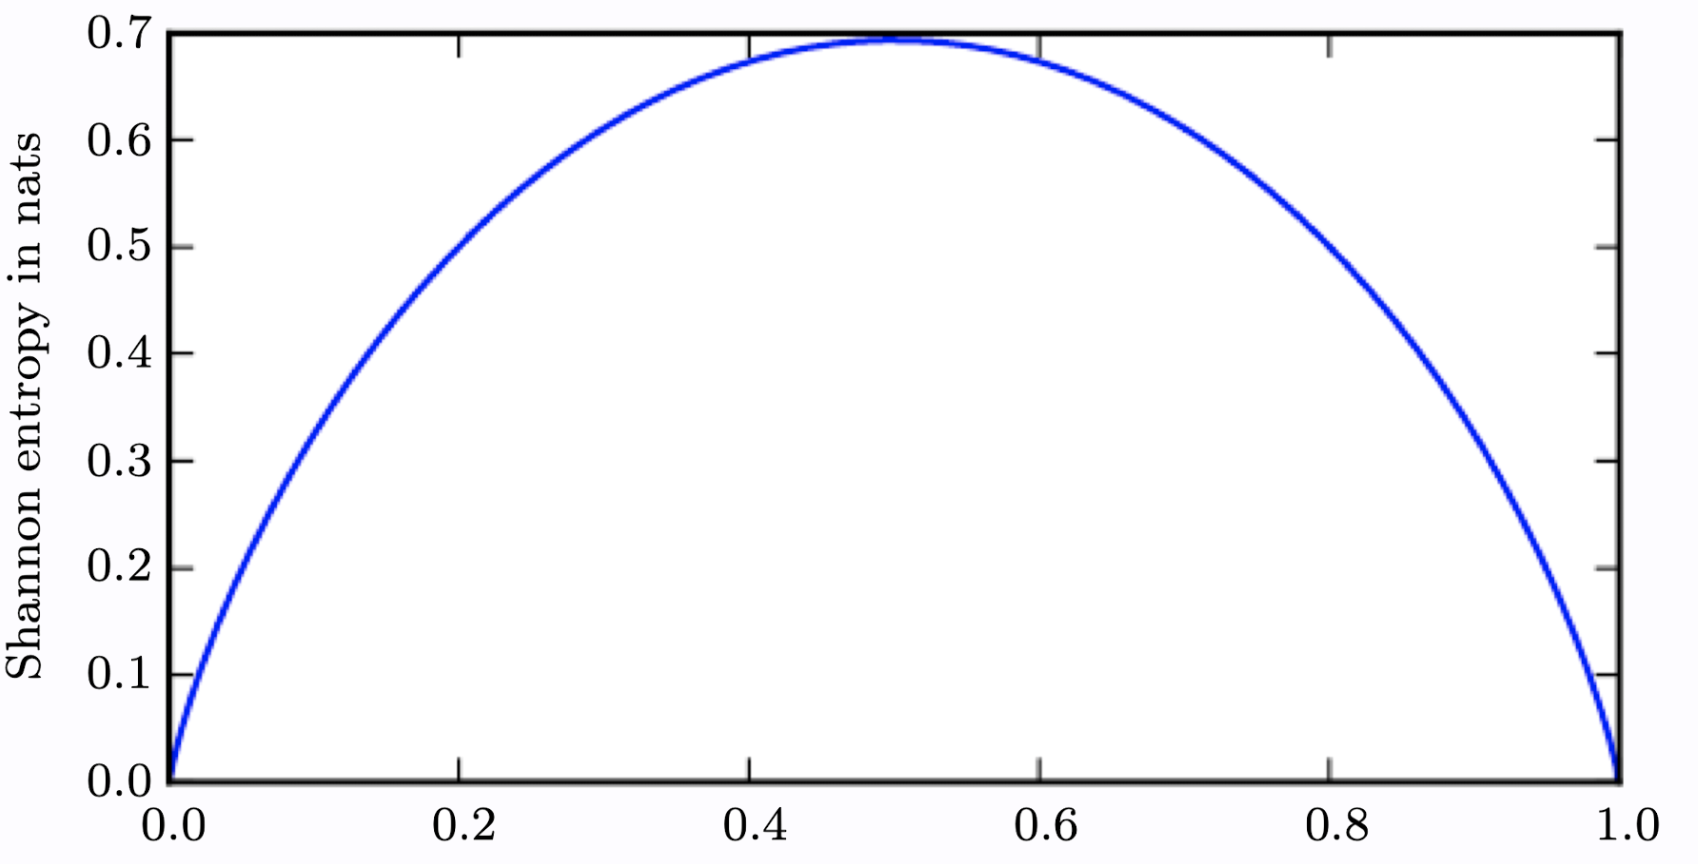
\includegraphics[scale=.5]{images/prerequisites/shannon.png}
    \caption{L'entropia di una variabile casuale \textbf{x}$\sim$\textbf{Bernoulli}($\phi$) al variare di $\phi$ tra $0$ e $1$.}
    \centering
\end{figure}


\paragraph{La divergenza Kullback-Leibler(KL).} Se abbiamo due distribuzioni separate $P(\text{x})$ e $Q(\text{x})$ della stessa variabile x, possiamo misurare quanto siano differenti l'una dall'altra utilizzando la \textbf{Kullback-Leibler divergence}:
\begin{equation}
    D_{\text{KL}}(P\|Q)=E_{\text{x}\sim P}\Big[ \log\frac{P(x)}{Q(x)} \Big]=E_{\text{x}\sim P}[\log P(x)-\log Q(x)].
\end{equation}
Nel caso di variabili discrete, rappresenta la \textbf{quantità extra di informazioni} di cui si necessita per inviare un messaggio contenente simboli estratti dalla distribuzione di probabilità $P$, quando usiamo codice il cui design è pensato per minimizzare la lunghezza di messaggi estratti dalla distribuzione di probabilità $Q$.



\paragraph{Proprietà della KL divergence.}
\begin{itemize}
    \item la KL divergence è sempre \textbf{non negativa};
    \item la KL divergence è $0\Longleftrightarrow P$ e $Q$ sono la stessa distribuzione (o sono ugali \textit{quasi in ogni punto} nel caso di variabili continue);
    \item la KL divergence \textbf{non è una misura di distanza}: una distanza dovrebbe essere simmetrica e soddisfare la disuguaglianza triangola, ma la KL divergence non o fa.
\end{itemize}
Quest'ultimo punto, in particolare il fatto che non sia simmetrica, ha importanti conseguenza quando bisogna minimizzare la \textbf{distanza} tra le due distribuzioni $P$ e $Q$.



\paragraph{Minimizzare la KL divergence.} Minimizzare $D_{\text{KL}}(p\|q)$ può essere molto diverso da minimizzare $D_{\text{KL}}(q\|p)$.
Assumiamo che:
\begin{itemize}
    \item $p$ sia una mistura di due Gaussiane con 2 diverse mode;
    \item $q$ sia una singola Gaussiana che vogliamo \textbf{ottimizzare} in modo che matchi $p$ nel modo migliore possigile.
\end{itemize}
\begin{equation}
     D_{\text{KL}}(p\|q)=E_{\text{x}\sim p}\Big[ \log\frac{p(x)}{q(x)}\Big].
\end{equation}
\begin{figure}[!h]
    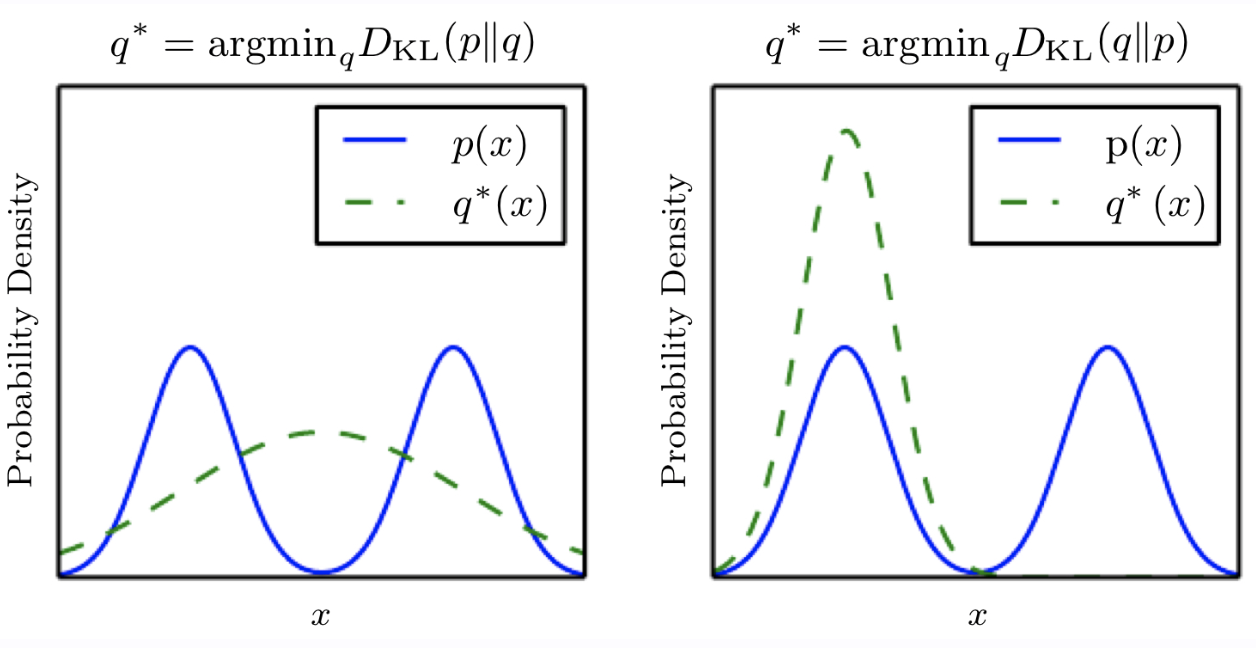
\includegraphics[scale=.6]{images/prerequisites/kl01.png}
    \centering
\end{figure}
\begin{equation}
     D_{\text{KL}}(q\|p)=E_{\text{x}\sim q}\Big[ \log\frac{q(x)}{p(x)}\Big].
\end{equation}
\newpage
\begin{equation}
    \min_q[D_{\text{KL}}(p\|q)]=\min_q\Big[ \mathbb{E}_{\text{x}\sim p}\Big[\log\frac{p(x)}{q(x)} \Big]\Big]
\end{equation}
\begin{figure}[!h]
    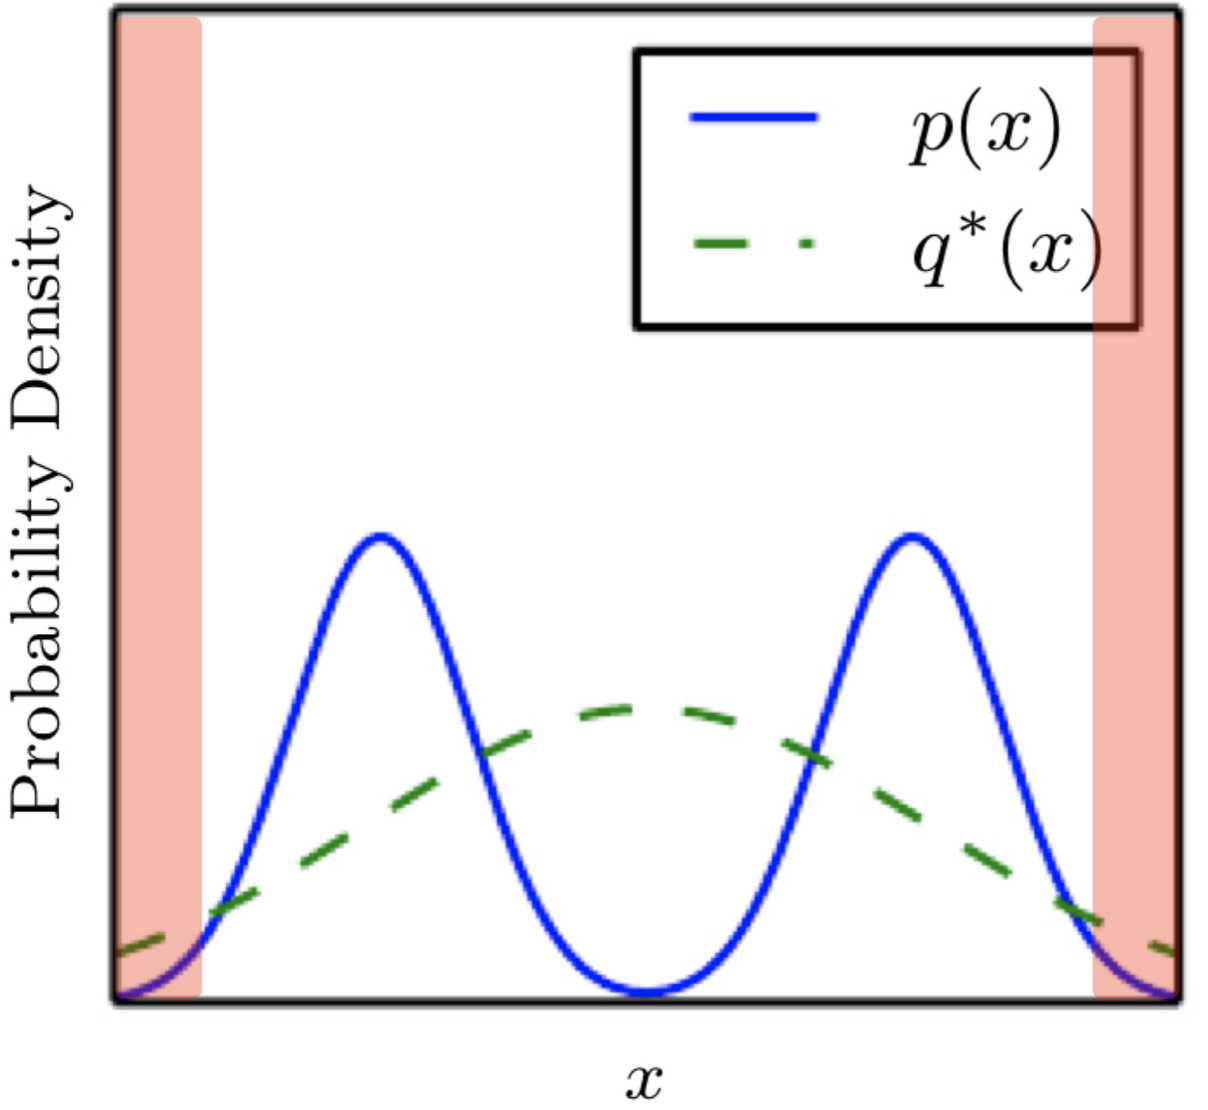
\includegraphics[scale=.5]{images/prerequisites/kl02.png}
    \centering
\end{figure}
\begin{equation}
    \min_q[D_{\text{KL}}(q\|p)]=\min_q\Big[ \mathbb{E}_{\text{x}\sim q}\Big[\log\frac{q(x)}{p(x)} \Big]\Big]
\end{equation}
\begin{figure}[!h]
    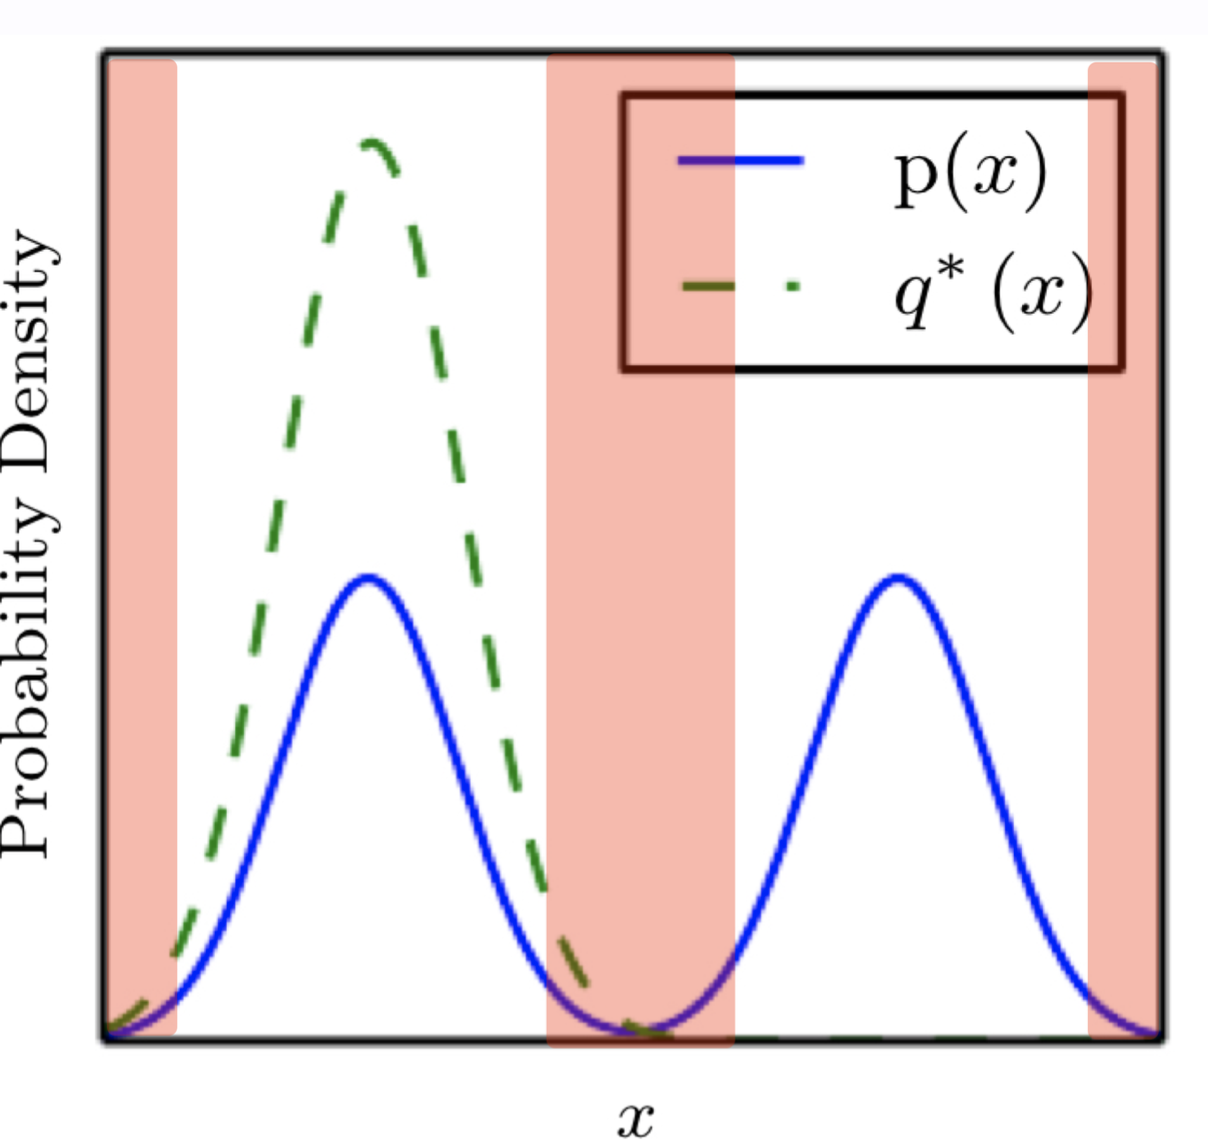
\includegraphics[scale=.5]{images/prerequisites/kl03.png}
    \centering
\end{figure}
\newpage
\paragraph{Cross Entropy.} Una quantità che è strettamente correlata alla KL divergence è la \textbf{cross-entropy}:
\begin{equation}
    H(P,Q)=H(P)+D_{\text{KL}}(P\|Q)=-E_{\text{x}\sim P}[\log Q(x)]
\end{equation}
cioè la cross entropy è \textbf{il numero medio di bit necessari per codicare un messaggio del codice $Q$ con un codice pensato per $P$}.


\textbf{Note:}
\begin{itemize}
    \item è simile a $D_{\text{KL}}(P\|Q)=E_{\text{x}\sim P}[\log P(x)-\log Q(x)]$:
    \begin{itemize}
        \item expressioni simili ma manca il termine $\log Q(x)$;
        \item concettualmente differente è il fatto che $D_{\text{KL}}$ misuri il numero di bit extra previsto mentre $H$ misuri il numero totale di bit.
    \end{itemize}
    \item minimizzare $H(P,Q)$ rispetto a $Q$ è la stessa cosa di minimizzare $D_{\text{KL}}(P\|Q)$. 
\end{itemize}    
    
Il motivo si vede bene guardando il fattore $H(P)+D_{\text{KL}}(P\|Q)$; infatti quando minimizziamo $P$ e $Q$ lo facciamo rispetto alla distribuzione $Q$, in questo fattore si vede bene che c'è un termine, $H(P)$, che non dipende dalla distribuzione $Q$, e il secondo termine, che è esattamente la KL, che invece dipende da $Q$. Perciò sostanzialmente stiamo andando a minimizzare la KL anche quando minimizziamo la cross-entropy. \textbf{Il punto è che spesso è più semplice minimizzare la cross-entropy perchè ha una forma più semplice rispetto alla KL.}

\newpage

\subsection{Modelli grafici (modelli probabilistici strutturati)}
Spesso le distribuzioni di probabilità possono essere divise in molti fattori. Per esempio, assumiamo che un variabile casuale $a$ influenzi il valore di un'altra variabile $b$ e che questa a sua volta influenzi $c$, ma sono indipendeti l'una rispetto all'altra. Possimo rappresentare l'intera distribuzione come segue:
\begin{equation}
    p(a,b,c)=p(a)p(b|a)p(c|b).
\end{equation}
Questi tipi di fattorizzazione possono \textbf{ridurre enormemente il numero di parametri} necessari per descrivere una distribuzione.
\newline
\newline
\textbf{Esempio:}


Assumiamo che $a,b,c$ assumano tutte valori in $\{1,2,3,4,5\}$. Per descrivere completamente le probabilità coinvolte dovremmo specificare $5^3=125$ valori di probabilità.


Se la distribuzione fattorizza come sopra abbiamo bisogno solo di:
\begin{itemize}
    \item $5$ parametri per descrivere $p(a)$;
    \item $25$ parametri per descrivere $p(b|a)$;
    \item $25$ parametri per descrivere $p(c|b)$.
\end{itemize}

\paragraph{Modelli grafici.} Le fattorizzazioni sulle distribuzioni possono essere visivamente descritti usando i grafi.
\paragraph{Modelli diretti.} Utilizzano grafi con archi diretti. Rappresentano le fattorizzazioni in distribuzioni di probabilità condizionate:
\begin{itemize}
    \item un fattore per ogni variabile casuale x$_i$;
    \item il fattore consiste nella distribuzione condizionata di x$_i$ dato dai genitori.
\end{itemize}
\begin{equation}
    p(\text{x})=\prod_i p(\text{x}_i|Pa_{\mathcal{G}}(\text{x}_i))
\end{equation}
dove $Pa_{\mathcal{G}}(\text{x}_i)$ è l'insieme dei genitori di x$_i$.
\begin{figure}[!h]
    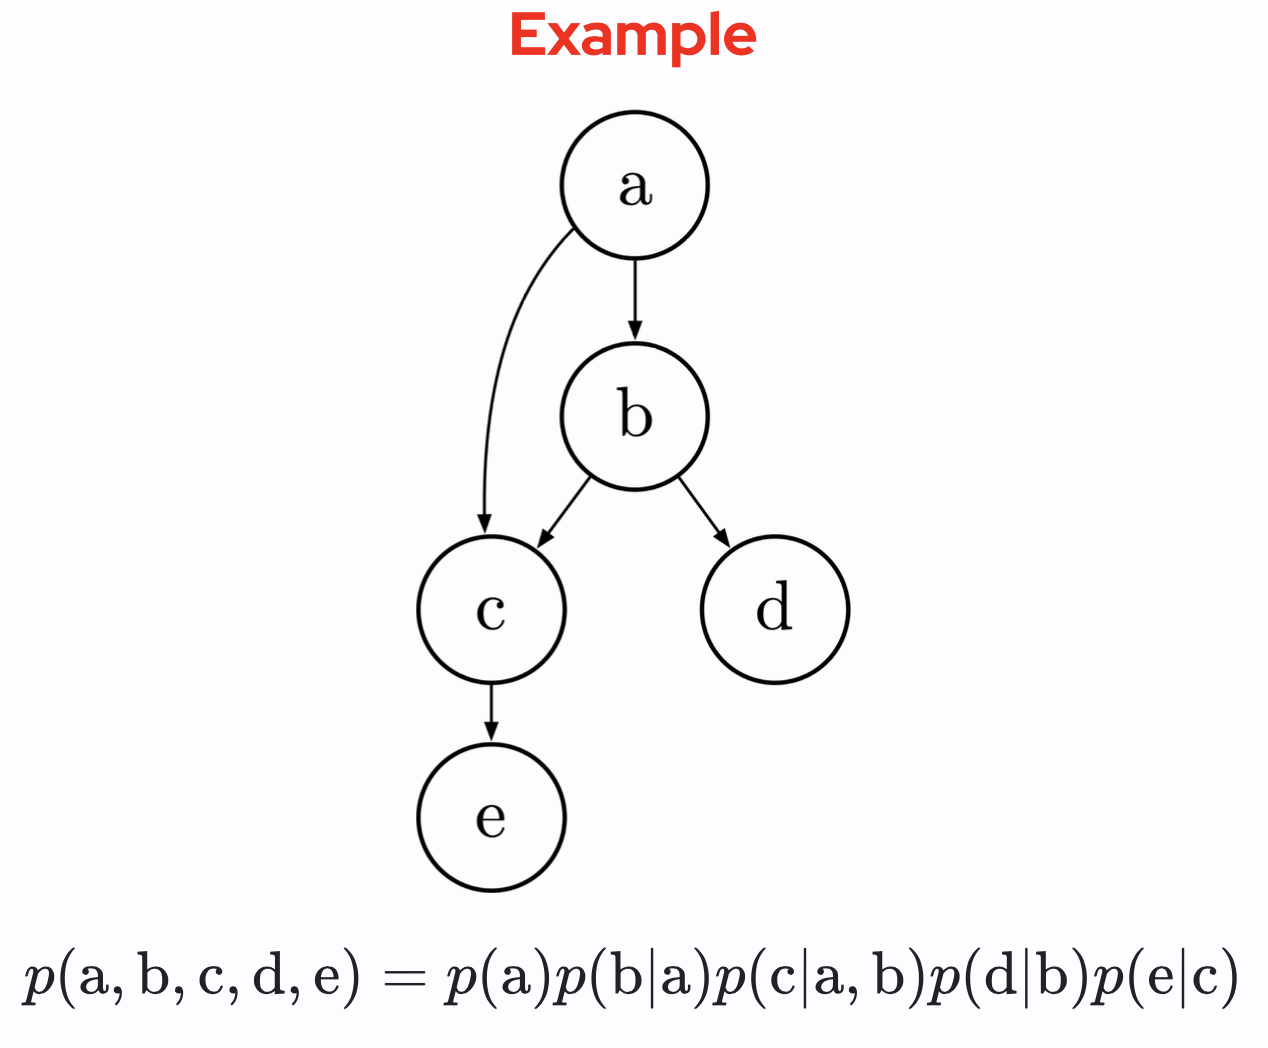
\includegraphics[scale=.5]{images/prerequisites/graphModelDir.png}
    \centering
\end{figure}
\newpage
\paragraph{Modelli indiretti.} Utilizzano grafi con archi indiretti. Rappresentano la fattorizzazione utilizzando un insieme di funzioni (non necessario né comune che siano distribuzioni probabilistiche):
\begin{itemize}
    \item c'è un fattore $\phi^{i}$ per ogni clique\footnote{sottografo completamente connesso.} $\mathcal{C}^{(i)}$ del grafo;
    \item la fattorizzazione è il prodotto normalizzato di tutti i fattori.
\end{itemize}
\begin{equation}
    p(\text{x})=\frac{1}{Z}\prod_i\phi^{(i)}(\mathcal{C}^{(i)}),
\end{equation}
con $Z=\sum_{x\in\text{x}}\prod_i\phi^{(i)}(\mathcal{C}^{(i)})$ fattore di normalizzazione.
\begin{figure}[!h]
    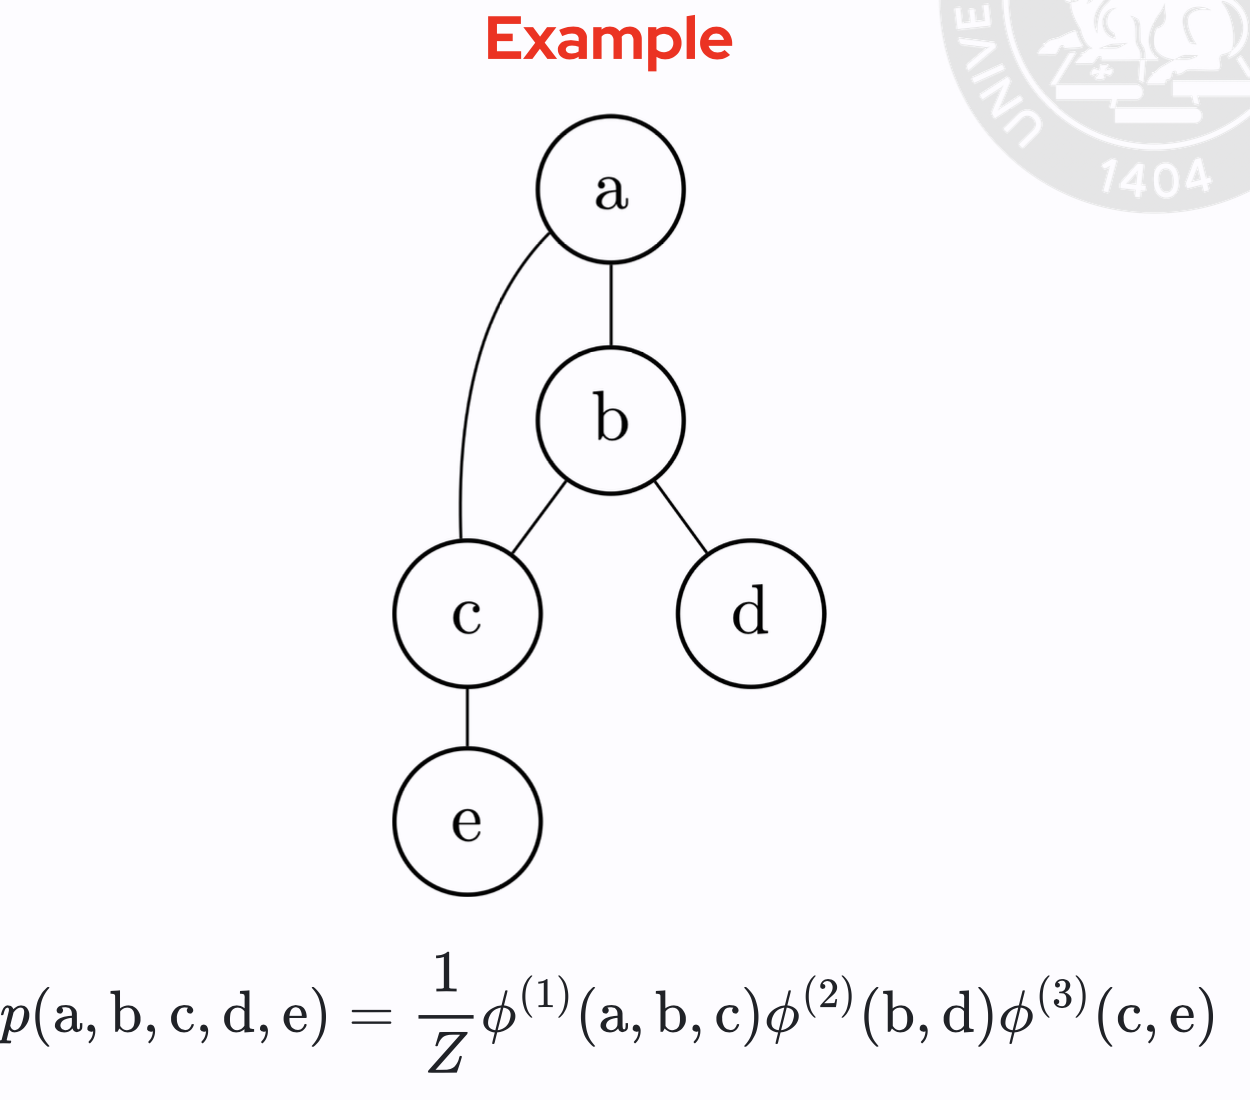
\includegraphics[scale=.5]{images/prerequisites/graphModelUnd.png}
    \centering
\end{figure}
\newpage
\clearemptydoublepage
% %% CHAPTERS
% add any further chapter file here
%\chapter{Percettrone}
E' stato introdotto da Frank Rosenblatt, uno psicologo americano, nel 1958.



Si tratta di una semplice forma di rete neurale utilizzata per \textbf{classificare esempi linearmente separabili}.



È possibile trovare un \textbf{iperpiano} che \textbf{separi} tutti gli esempi classificati in un modo da tutti quelli classificati in un altro modo.


Un esempio:
\begin{figure}[!h]
    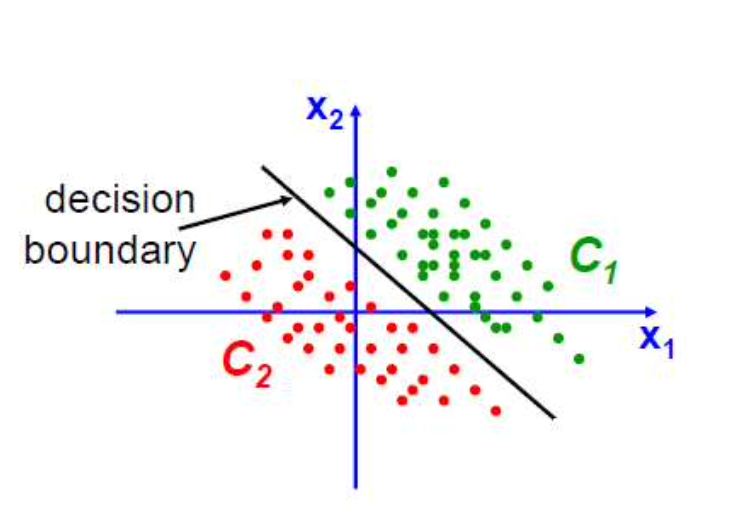
\includegraphics[scale=.5]{images/perceptron/perceptron.png}
    \centering
\end{figure}



La \textbf{struttura} del percettrone è la seguente:
\begin{itemize}
    \item \textbf{input}, il vettore \textbf{x};
    \item \textbf{output}, il vettore \textbf{y} (un singolo valore se si tratta di un neurone);
    \item \textbf{vettore dei pesi}, il vettore \textbf{w}.
\end{itemize}
\begin{figure}[!h]
    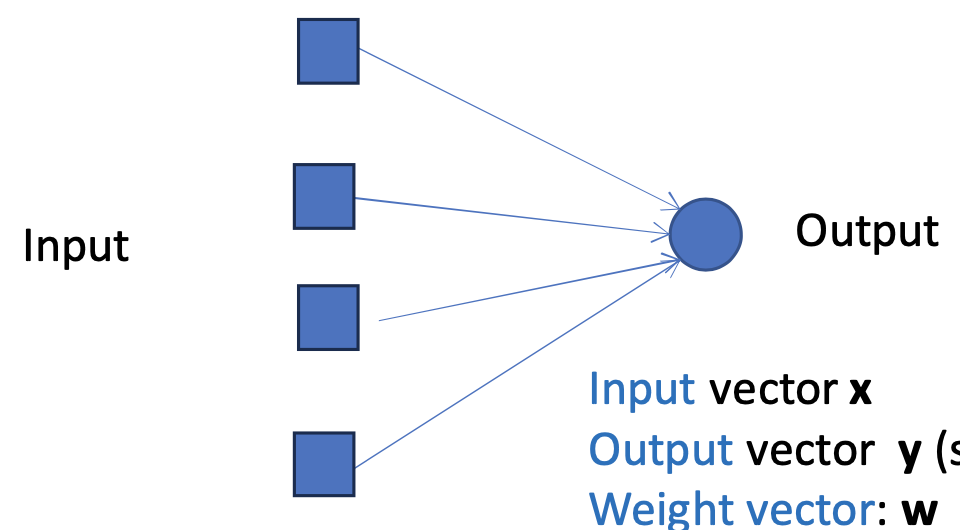
\includegraphics[scale=.5]{images/perceptron/struct.png}
    \centering
\end{figure}

Il \textbf{training set} è formato da coppie:\newline
[\textit{
(input$_1$,outputDesiderato$_1$),\newline
(input$_2$,outputDesiderato$_2$),\newline
$\dots$
}].
\newpage
\section{Principi basici delle reti neurali}
Nel cervello umano, \textbf{l'unita computazionale basica} è il \textbf{neurone}. Ci sono circa $10$ miliardi di neuroni e $60$ milioni di milioni di sinapsi.



Esattamente allo stesso modo, \textbf{anche l'unita computazionale basica delle reti neurali è il neurone}. Ed anche qui, molti neuroni sono connessi gli uni agli altri tramite le sinapsi.
\begin{figure}[!h]
    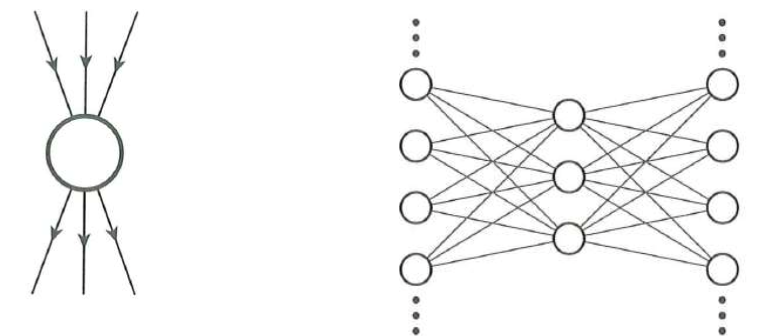
\includegraphics[scale=1]{images/perceptron/neuron01.png}
    \centering
\end{figure}



Il princpale ruolo di un neurone all'interno del cervello è quello di raccogliere, elaborare e propagare i segnali elettrici.
Il segnale elettrico in output è proporzionale al segnale in input ricevuto.



Di nuovo, esattamente allo stesso modo, \textbf{il neurone formale riceve, elabora e trasmette ai neuroni successivi l'informazione ricevuta. L'output è proporzionale all'input ricevuto}.


Le operazioni del singolo neurone \textbf{sono molto semplici}: ad esempio decidere se l'input totale è superiore o meno ad una soglia.
\begin{figure}[!h]
    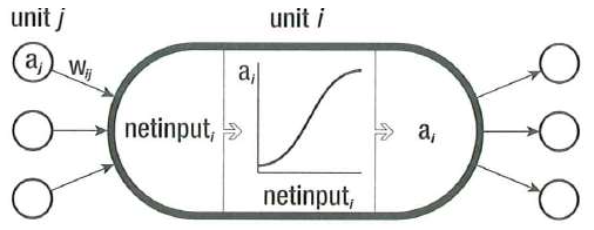
\includegraphics[scale=1]{images/perceptron/neuron02.png}
    \centering
\end{figure}
\newpage
\textbf{Neurone (McCulloch Pitts 1943)}
\begin{figure}[!h]
    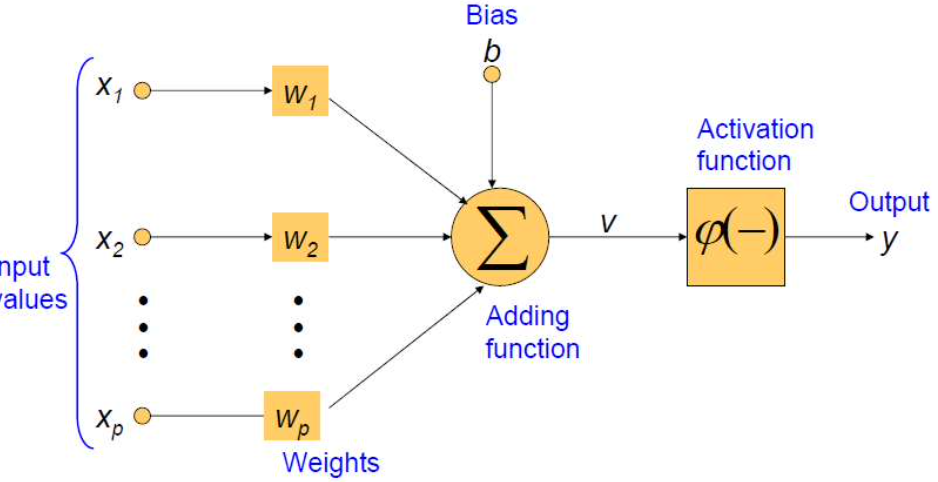
\includegraphics[scale=1]{images/perceptron/pitts.png}
    \centering
\end{figure}


\begin{itemize}
    \item vettore di input \textbf{x}
    $\begin{bmatrix}
        x_1\\
        \dots\\
        x_p
    \end{bmatrix}$;
    \item vettore dei pesi \textbf{w}
    $\begin{bmatrix}
        w_1\\
        \dots\\
        w_p
    \end{bmatrix}$.
\end{itemize}
Per ogni valore di input $x_i$, ciò che il neurone $j$ riceve è $w_{ji}x_i$. 


$w_{ji}x_i$ è il peso della sinapsi da $i$ a $j$. Così come una sinapsi può essere eccittata o inibita, così anche un peso può essere maggiore, minore o uguale a zero.
\newline
\newline
Il cosiddetto \textbf{network input} o (\textbf{netinput}) di $j=\text{\textbf{x}}\cdot\text{\textbf{w}}$ ($=\text{\textbf{x$^{\text{T}}$}}\cdot\text{\textbf{w}}=\sum_{i=1}^p\text{x}_i\text{w}_i$).
\newline
\newline
Alcune esempi di valori in input sono:
\begin{itemize}
    \item pixel values;
    \item fonemi;
    \item misurazioni;
    \item encoding di concetti di livello superiore;
    \item encoding di single parole;
    \item output di altri neuroni.
\end{itemize}
L'output del neurone dipenderà dal \textbf{netinput e dal bias}:
\begin{equation}
    y_j=\phi(u_j+b)
\end{equation}
dove $u_j+b$ rappresenta il potenziale di attivazione o campo locale di $j$.
\newpage
Tutti i neuroni hanno un \textbf{bias} che rappresenta la loro attivazione spontanea:
\begin{itemize}
    \item se bias$>0$ il neurone è spesso attivo, anche con input bassi;
    \item se bias$<0$, affinché il neurone sia attivo, i valori di input devono essere alti (rappresenta infatti una soglia).
\end{itemize}


\begin{figure}[!h]
    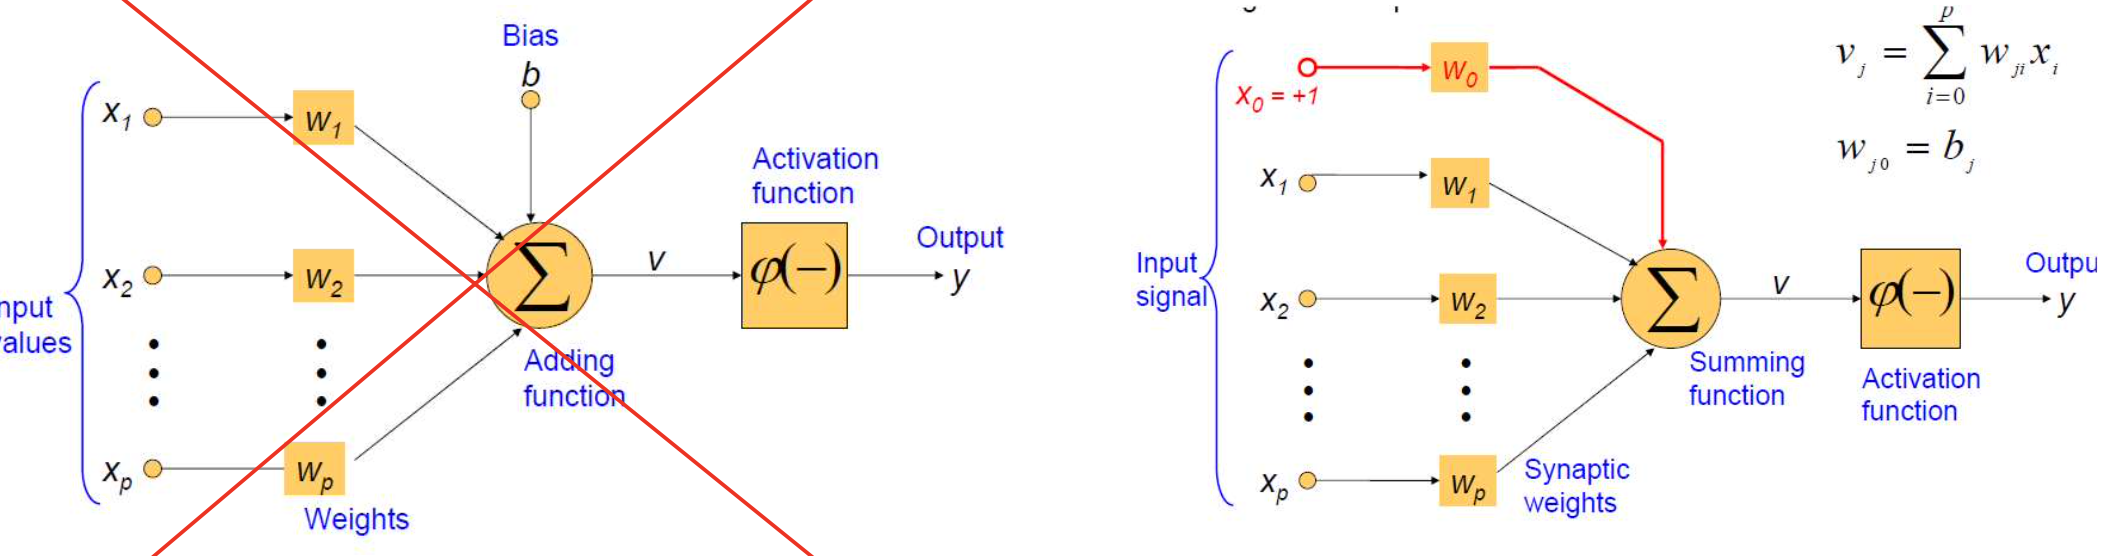
\includegraphics[scale=.4]{images/perceptron/architecture.png}
    \centering
\end{figure}


Per semplificare i calcoli, il bias del neurone $j$ può essere trattato come un elemento aggiuntivo in input  $\text{x}_0 =1$ con $\text{w}_0 =b$.
\newline
In questo caso, $\text{v}_j=\sum_{j=0}^p\text{v}_{\text{ji}}\text{x}_\text{i}$. \newline
Questa sarà l'architettura che noi utilizzeremo.\newline
\newline
\textbf{Esempio:}\newline
L'\textbf{or}, normalmente rappresentato così
\begin{gather}
    ([1,1], 1)\\
    ([1,0], 1)\\
    ([0,1], 1)\\
    ([0,0], -1)
\end{gather}
si traformerà in questo
\begin{gather}
    ([1,1,1], 1)\\ 
    ([1,1,0], 1)\\
    ([1,0,1], 1)\\
    ([1,0,0],-1).
\end{gather}
\newpage
\paragraph{La funzione di attivazione.}
Riguardo questa funzione:
\begin{itemize}
    \item l'output del percettrone sarà $1$ se $\sum_{i=0}^px_{ji}x_i>0$ (cioè se $\textbf{x}\cdot\textbf{w}>0$);
    \item l'output del percettrone sarà $-1$ se $\sum_{i=0}^px_{ji}x_i\leq0$ (cioè se $\textbf{x}\cdot\textbf{w}\leq0$).
\end{itemize}
\begin{figure}[!h]
    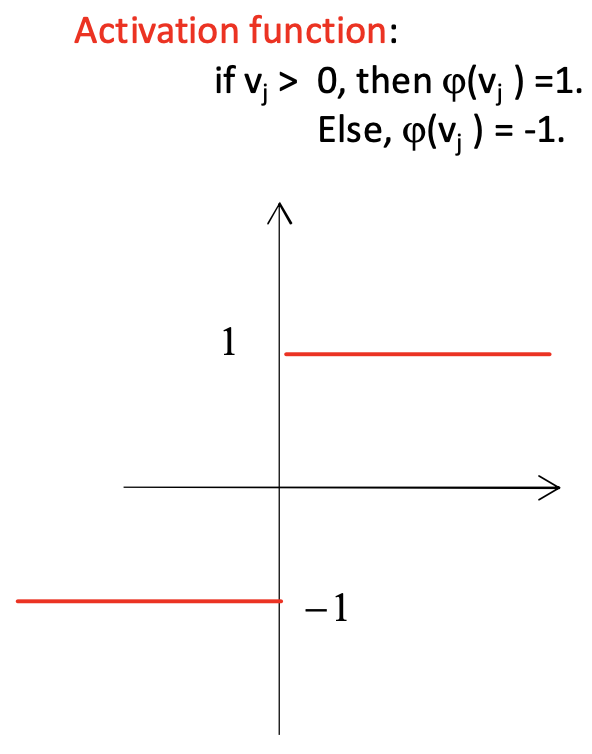
\includegraphics[scale=.4]{images/perceptron/actFun.png}
    \centering
\end{figure}


Perciò si può dire che \textbf{l'output del percettrone per un dati input dipende dal vettore dei pesi}. Infatti, data una certa configurazione \textbf{w}:
\begin{itemize}
    \item l'output sarà $1$ per tutti i vettori di input \textbf{x} tali che $\textbf{x}\cdot\textbf{w}>0$;
    \item l'output sarà $-1$ per tutti i vettori di input \textbf{x} tali che $\textbf{x}\cdot\textbf{w}\leq0$.
\end{itemize}
\begin{figure}[!h]
    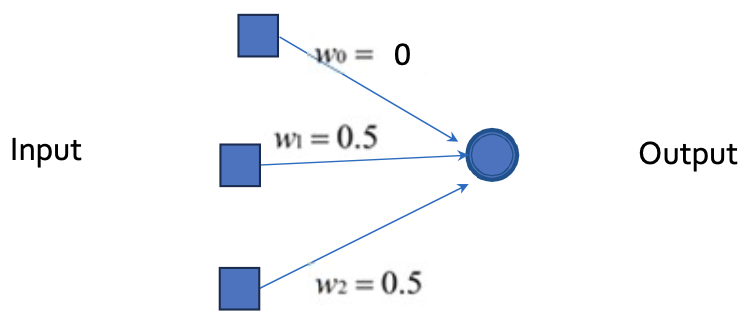
\includegraphics[scale=.8]{images/perceptron/weight.png}
    \centering
\end{figure}


Il \textbf{decision boundary} è dato da tutti gli \textbf{x} tali che $\textbf{x}\cdot\text{w}=0$.
\newline
\newline
Un esempio di una possibile soluzione per l'or è dato da $\textbf{w}_1=\textbf{w}_2=0.5$,$\textbf{w}_0=0$
\begin{figure}[!h]
    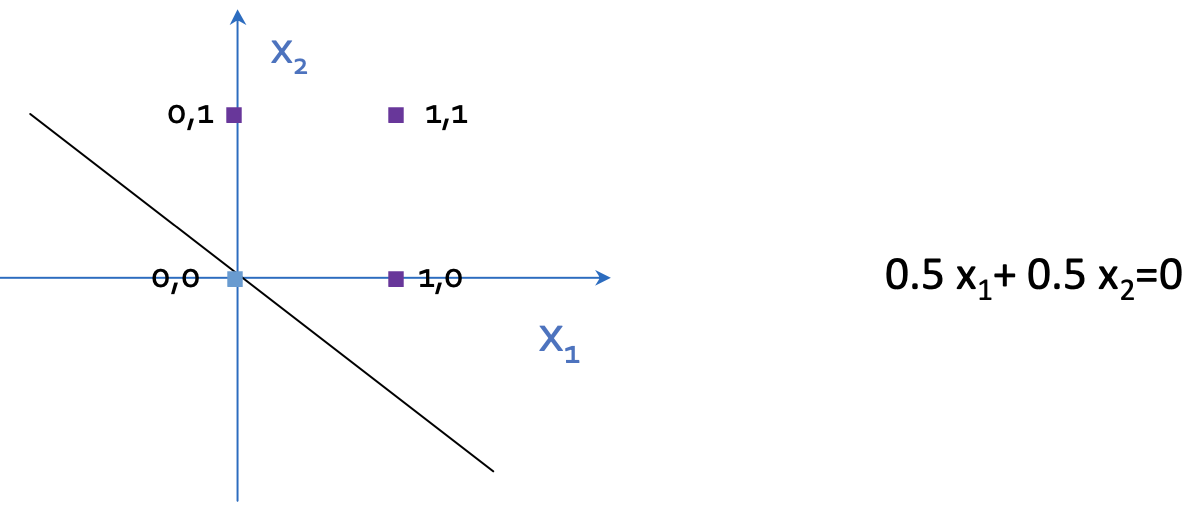
\includegraphics[scale=.5]{images/perceptron/orSolution.png}
    \centering
\end{figure}
\newpage
Il \textbf{percettrone} impara a classificare gli esempi \textbf{linearmente separabili} regolando i pesi. Gli esempi sono coppie (\textit{input, output desiderato}) che costituiscono il \textbf{training set}. Gli esempi (anche detti \textbf{pattern}) si trovano all'interno del training set. Nelle reti più complesse può essere utilizzato anche un \textbf{test set} per testare l'apprendimento della rete su un set di esempi diversi da quelli presenti nel training set.
\section{Learning Algorithm}
Il modo con cui il percettrone ottiene l'output desiderato è \textbf{modificando i pesi}. Questa modifica è ottenuta grazie all'applicazione di un algoritmo di learning basato, per esempio, \textbf{sulla correzione degli errori}. Segue la regola per la correzione dei pesi dell'$n$-esima iterazione:
\begin{itemize}
    \item $w(n+1) = w(n)$ se l'output è corretto;
    \item se l'output non è corretto:
    \begin{itemize}
        \item se l'output è minore del previsto\newline $w(n+1) = w(n) - \eta(n)x(n)$ se $x(n) \cdot w(n) > 0$ e $x(n) \in C2$;
        \item se l'output è maggiore del previsto\newline $w(n+1) = w(n) +\eta(n)x(n)$ se $x(n) \cdot w(n) \leq 0$ e $x(n) \in C1$.
    \end{itemize}
\end{itemize}
L'algoritmo continua finché ci sono elementi non classificati correttamente.\newline
%psudocodice%
Un'\textbf{epoca} è un'iterazione su tutti gli elementi del set di addestramento. Qui l'aggiornamento del peso avviene \textbf{pattern-by-pattern}: i pesi vengono aggiornati per ogni patterb classificato erroneamente.
\newline
L'algoritmo può anche essere semplificato in questo modo:
%pseudo algoritmo semplificato%
\newpage
\section{Teorema della convergenza}
Se esiste una soluzione (ovvero se il problema è linearmente separabile), l'algoritmo la trova. \newline
Ad ogni iterazione viene modificato il vettore dei pesi e, di conseguenza, il decision boundary. Il \textbf{Teorema della Convergenza garantisce che l’aggiustamento del peso termina}.
\begin{itemize}
    \item $\|w(k+1)\|^2\geq \frac{k^2\alpha^2}{\|w^*\|^2}$ (A) lower bound;
    \item $\|w(k+1)\|^2\leq k^2\beta^2$ (A) upper bound.
\end{itemize}
(A) e (B) sono compatibili se e solo se:
\begin{equation}
    \frac{k^2\alpha^2}{\|w^*\|^2}\leq k\beta,
\end{equation}
cioè
\begin{equation}
    k\leq \frac{\beta\|w^*\|^2}{\alpha^2}.
\end{equation}
\begin{figure}[!h]
    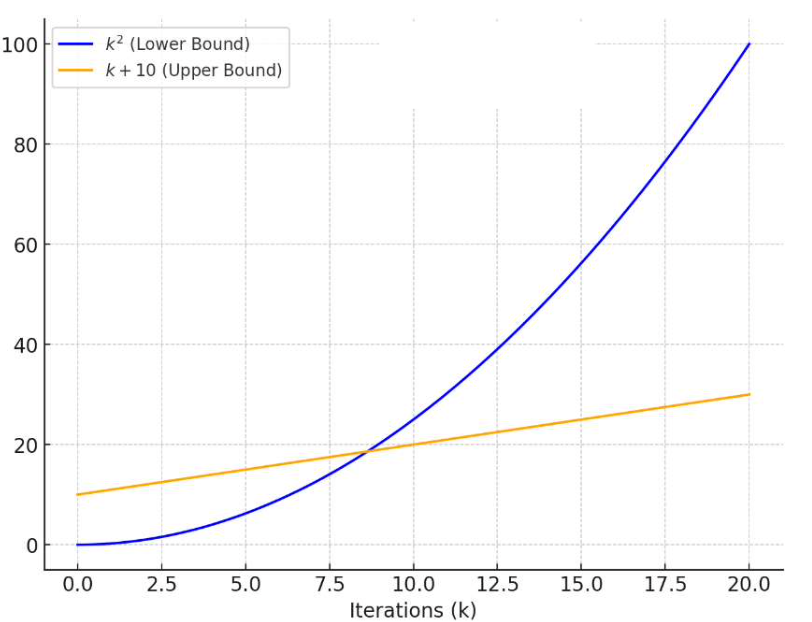
\includegraphics[scale=.8]{images/perceptron/convTheorem.png}
    \centering
\end{figure}
\newpage
\section{I limiti del percettrone e le Multilayer Networks}
Come precedentemente descritto e provato, il percettrone risolve problemi linearmente separabili come AND e OR. Ma come si comporta con i problemi che \textbf{non sono linearmente separabili} come, ad esempio, \textbf{lo XOR}?
\begin{figure}[!h]
    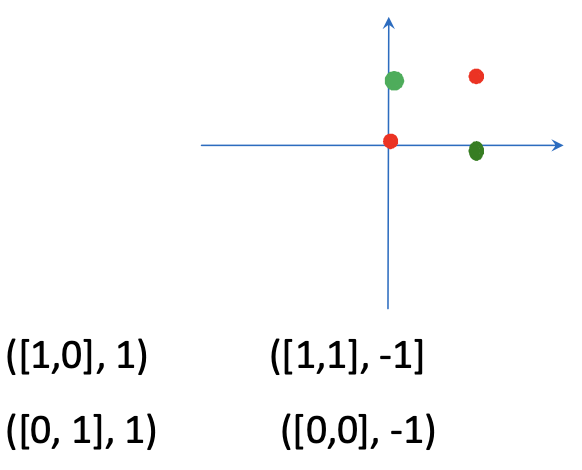
\includegraphics[scale=.8]{images/perceptron/xor.png}
    \centering
\end{figure}



Fondamentalmente, il percettrone non riesce e non può risolvere problemi di questo tipo. E la causa di ciò è proprio la natura di questi problemi, cioè il fatto che sia impossibile costruire una retta (piano, iperpiano ecc.) che separi perfettamente gli esempi del training set.\newline
Per risolverli bisogna introdurre i cosiddeti \textbf{hidden layer}, ognuno di quali risolve una parte del problema. Alla fine, si ha la costruzione della soluzione.
\begin{figure}[!h]
    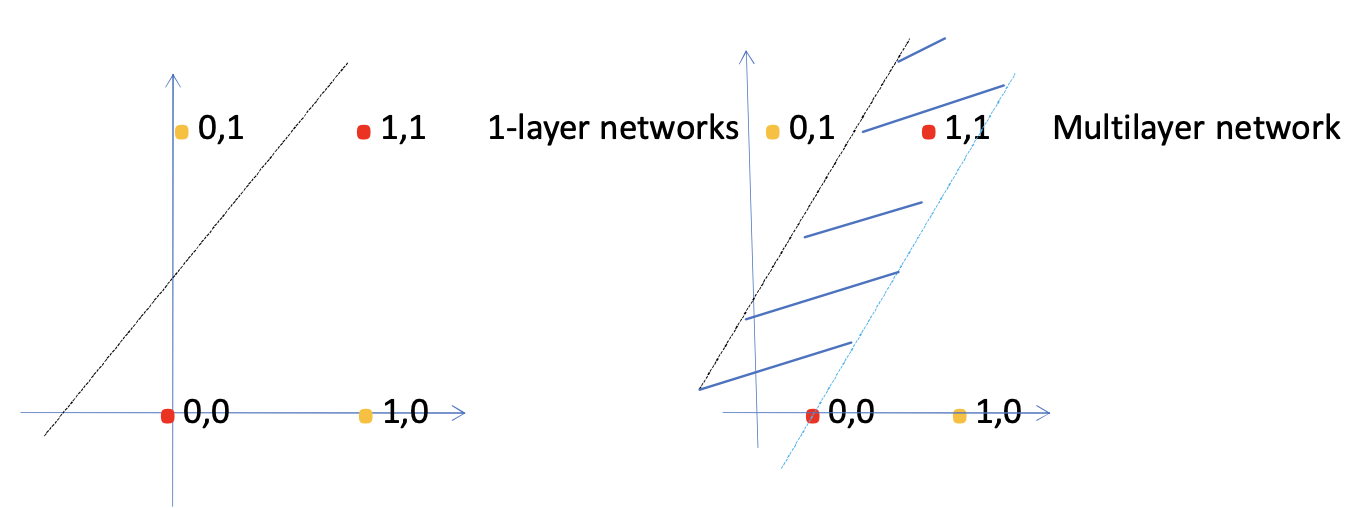
\includegraphics[scale=.75]{images/perceptron/multilayerNet.png}
    \centering
\end{figure}
\newpage


%\clearemptydoublepage
%\chapter{Discesa del gradiente}
\section{L’uso delle reti neurali per riconoscere caratteri scritti a mano}
Seppure la maggior parte delle persone riconosce facilmente le cifre scritte a mano 504192, la facilità di questo processo è estremamente ingannevole per due motivi:
\begin{itemize}
    \item In ogni emisfero del nostro cervello abbiamo una corteccia di visualizzazione primaria (chiamata V1) contenente circa 140 milioni di neuroni e miliardi di connessioni.
    \item Oltre alla V1 è presente un’intera serie di cortecce di visualizzazione (V2, V3, V4 e V5) le quali svolgono un processing completo dell’immagine in maniera progressiva.
\end{itemize}
\begin{figure}[!h]
    
\includegraphics[scale=.5]{images/gradient_descent/digit.png}
    \centering
\end{figure}




Proprio per questo motivo il riconoscimento di caratteri scritti a mano non è un processo semplice.
La difficoltà del visual pattern recognition diventa evidente se si cerca di realizzare un codice in grado di riconoscere le cifre come quelle mostrate nell’esempio precedente. Difatti ci sono semplici elementi che ci permettono di comprendere la cifra che non sono semplici da esprimere algoritmicamente. Ad esempio noi sappiamo che il numero 9 è formato da un cerchio posto in alto ed una linea dritta in basso a destra. Proprio questi elementi sono molto complessi da esprimere mediante un algoritmo. 
Il machine learning, e più precisamente le reti neurali, approcciano il problema in modi differenti. L’idea alla base è di prendere un gran numero di cifre scritte a mano da usare come esempi di training e successivamente sviluppare un sistema in grado di imparare dagli esempi.
\newpage
\section{Il Percettrone}
Il percettrone di Rosemblatt è la forma di rete neurale più semplice. 



(\textbf{Nota:} a seguire assumeremo che l’output del percettrone è $1$ se $w\cdot x+b>0$ e $0$\footnote{Questa definizione è leggermente imprecisa. Nella definizione originale gli output utilizzati sono $-1$ e $1$. Il cambio serve a semplificare la discussione e non modifica il ragionamento.} negli altri casi).
\begin{figure}[!h]
    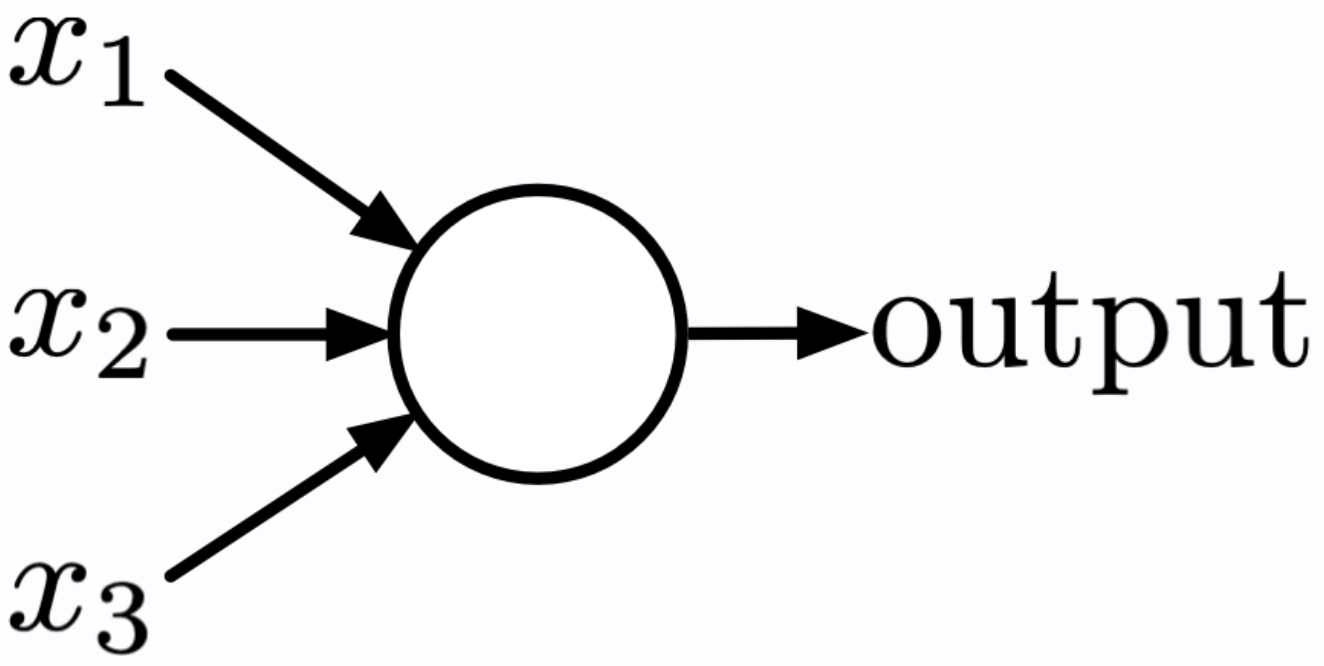
\includegraphics[scale=.4]{images/gradient_descent/perceptron.png}
    \centering
\end{figure}




Ovviamente un percettrone può esprimere concetti lineari molto semplici, ma sembra comunque plausibile che una rete complessa di percettroni possa effettuare delle decisioni più accurate. 
\begin{figure}[!h]
    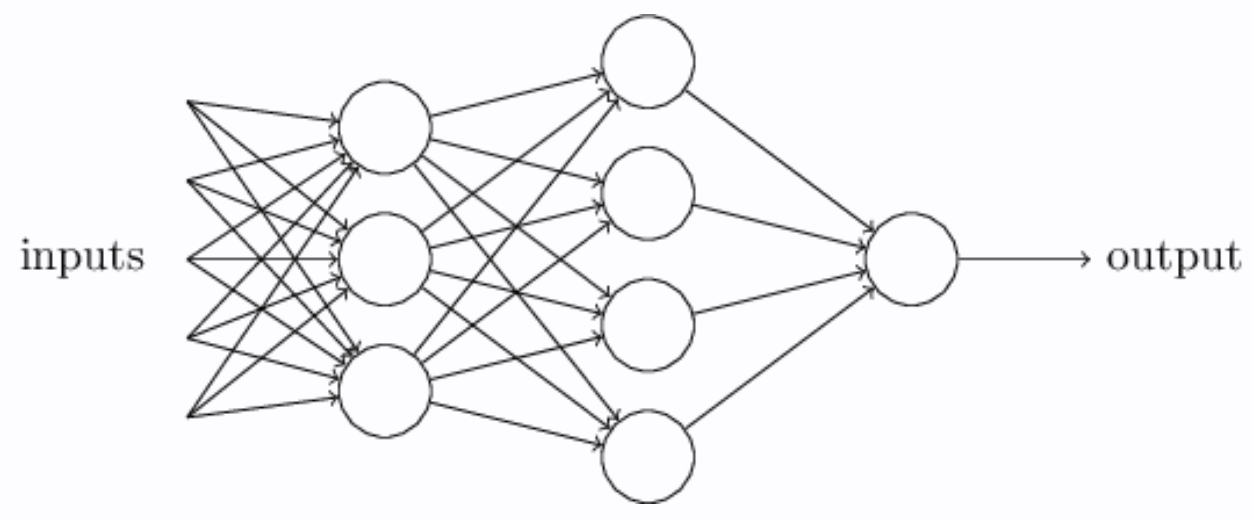
\includegraphics[scale=.4]{images/gradient_descent/perc_net.png}
    \centering
\end{figure}



Un altro modo in cui il percettrone può essere utilizzato è il calcolo delle funzioni logiche elementari. Per esempio, supponiamo di avere un percettrone con due input, ognuno con un peso di $-2$ e un bias totale di $3$.



Quale funzione booleana calcolerà questo percettrone?
\begin{figure}[!h]
    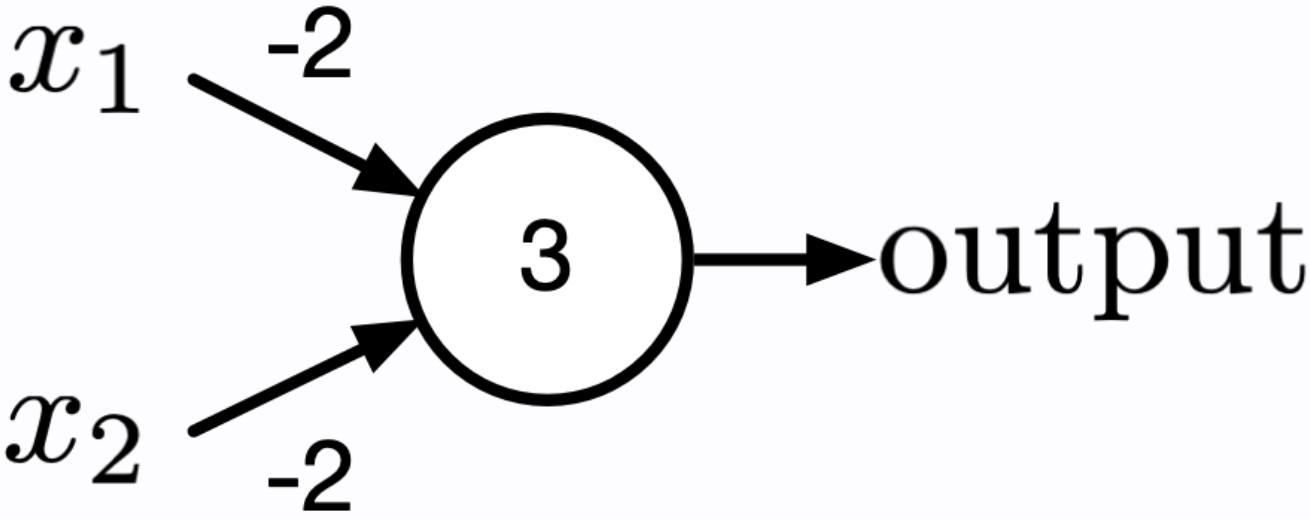
\includegraphics[scale=.4]{images/gradient_descent/perc_logic.png}
    \centering
\end{figure}
\newpage


Analizziamo come si comporta.
\begin{figure}[!h]
    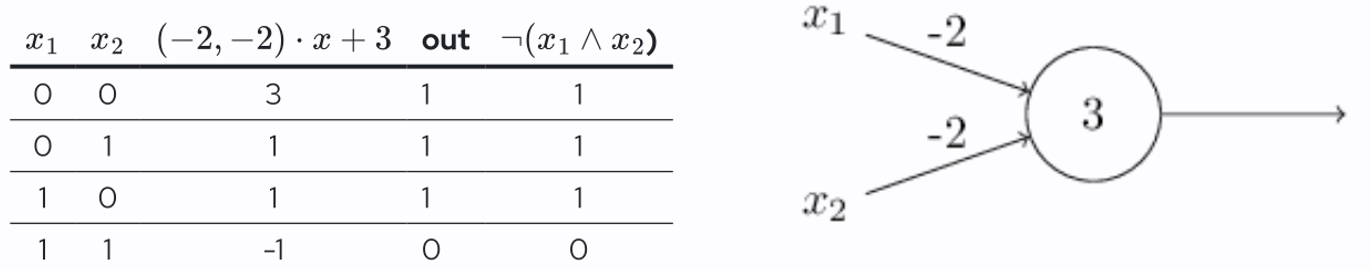
\includegraphics[scale=.7]{images/gradient_descent/nand.png}
    \centering
\end{figure}



Come sappiamo, l’esempio del NAND è particolarmente interessante perché può essere facilmente mostrato che qualsiasi altro operatore logico può essere costruito usando solamente i termini dell’operatore NAND.
Un esempio è il sommatore binario. 
\begin{figure}[!h]
    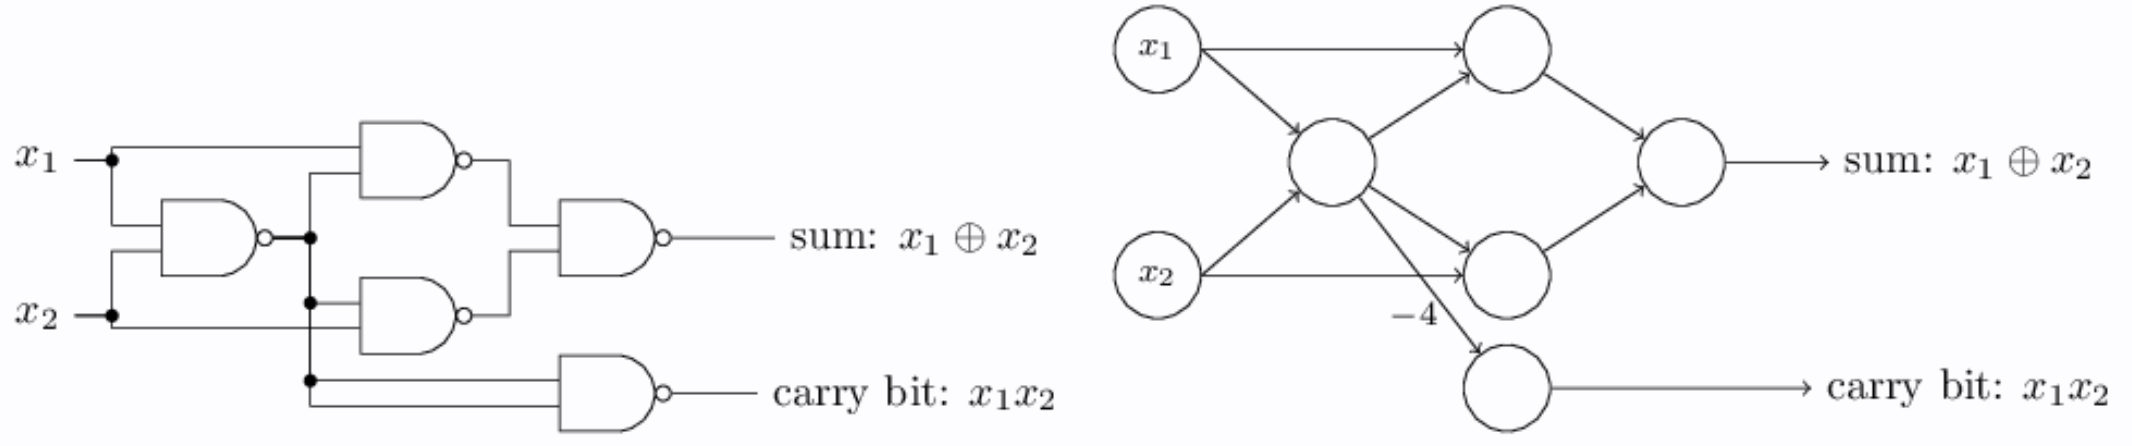
\includegraphics[width=170mm]{images/gradient_descent/bin_adder.png}
    \centering
\end{figure}



La teoria matematica delle reti neurali formalizza meglio quest’idea come la \textbf{Teoria dell’approssimazione universale}.

\newpage
\subsection{Teorema dell’approssimazione universale}
\paragraph{Def.} Una rete Feedforward con uno strato di output lineare e almeno uno strato nascosto con una qualsiasi funzione di attivazione “schiacciante” (come la funzione di attivazione del sigmoide logistico) può approssimare qualsiasi funzione misurabile di Boreal da uno spazio a dimensione finita a un altro con qualsiasi errore desiderato diverso da zero a condizione che alla rete siano fornite abbastanza unità nascoste. La derivata della rete feedforward può inoltre approssimare arbitrariamente bene le derivate della funzione.
\newline
\newline
Per i nostri scopi è sufficiente dire che qualsiasi funzione continua su un sottoinsieme chiuso e limitato è misurabile secondo Borel e quindi può essere approssimata mediante un metodo neurale rete.

\subsection{Limitazioni del teorema dell’approssimazione universale}
Sfortunatamente, nel peggiore dei casi, un numero esponenziale di unità nascoste (possibilmente con un’unita nascosta corrispondente ad ogni configurazione in ingresso che ha bisogno di essere distinta) può essere richiesto.
\newline
\newline
Questo problema è semplice da affrontare nel caso binario: il numero di possibili funzioni binarie sui vettori $v\in(0,1)^n$ è $2^{(2^n )}$ e la selezione di una di queste funzioni richiede $2^n$ bits, che generalmente richiede $O(2^n )$ gradi di libertà.
\begin{figure}[!h]
    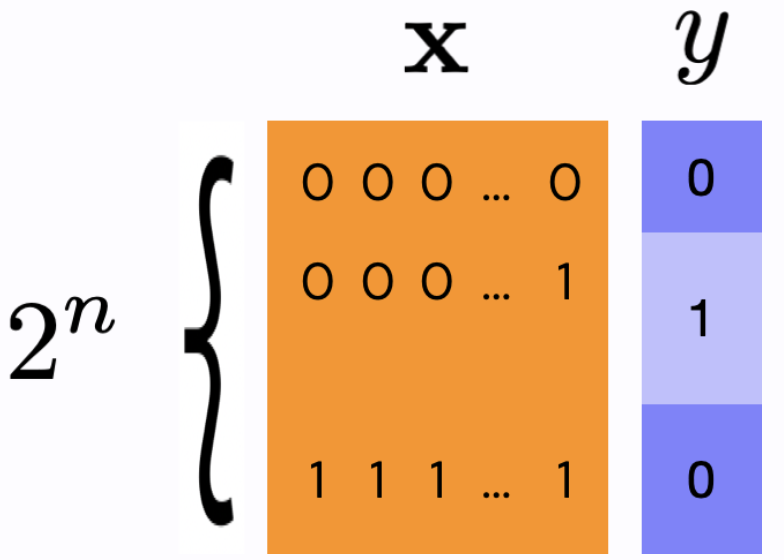
\includegraphics[scale=.8]{images/gradient_descent/limitation.png}
    \centering
\end{figure}
A questo punto sorge spontanea una domanda.


\textbf{Perché tutto ciò è così importante?}


Le risposte sono essenzialmente due:
\begin{itemize}
    \item perché le reti di percettroni possono eseguire qualsiasi tipologia di calcolo;
    \item \textbf{è possibile scrivere algoritmi in grado di imparare questi calcoli}.
\end{itemize}
\newpage
E' certamente però è molto difficile imparare qualcosa di utile utilizzando i percettroni.
\begin{figure}[!h]
    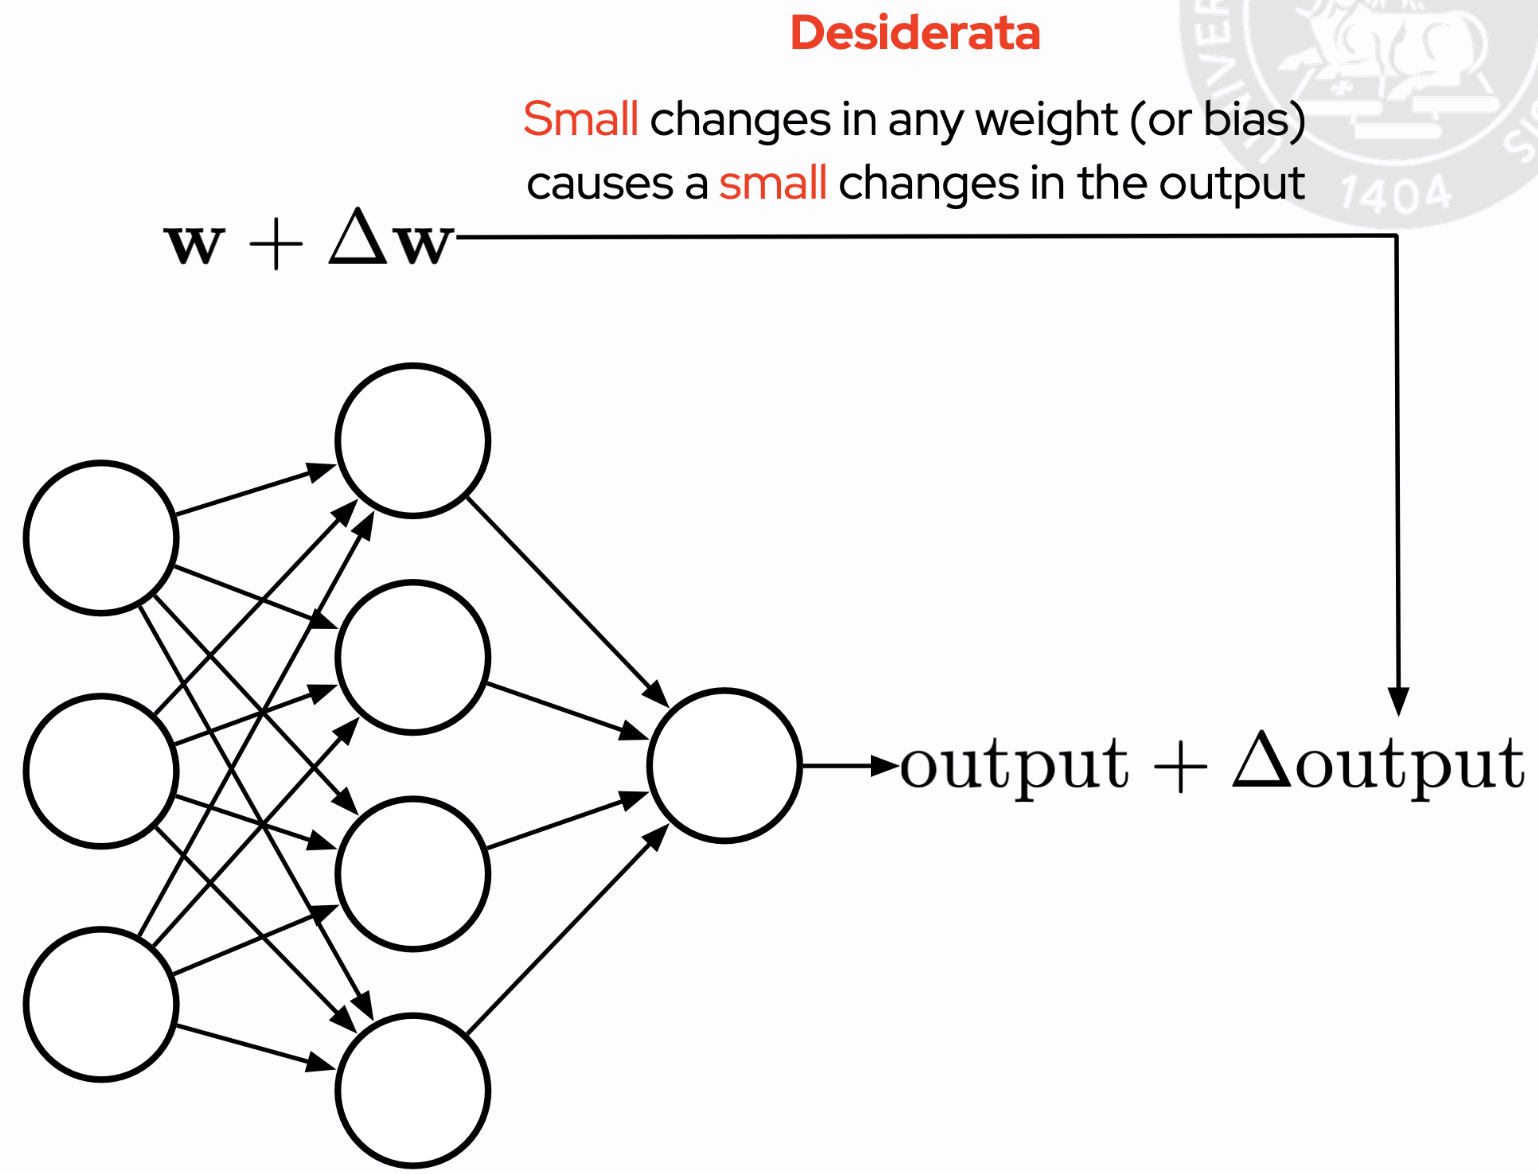
\includegraphics[scale=.3]{images/gradient_descent/sigmoid01.png}
    \centering
\end{figure}
\subsection{Neuroni sigmoide}
Un neurone sigmoide è definito come un neurone dove l’output è calcolato usando la formula: $\sigma(w\cdot x+b)$ dove $\sigma(z)=\frac{1}{(1+e^{-z})}$.
\textbf{Nota:}
\begin{itemize}
    \item gli output approssimano bene i passi della funzione quando $(w\cdot x+b)$ è estremamente grande o estremamente piccolo, ma  non cambia improvvisamente in prossimità di $0$;
    \item visto che il risultato è in $[0,1]$, gli input dei nodi interni prenderanno valori che vanno in $[0,1]$.
\end{itemize}
\begin{figure}[!h]
    \includegraphics[scale=.6]{images/gradient_descent/sigmoid02.png}
    \centering
\end{figure}


\textbf{Ricapitolando:} è importante che la \textbf{funzione di attivazione} sia regolare poiché vorremmo controllare come varia il $\Delta output$. Il calcolo è:
\begin{equation}
    \Delta output \approx\sum_j \frac{\partial output}{\partial w_j}\Delta w_j\frac{\partial output}{\partial b}\Delta b.
\end{equation}
Abbiamo inoltre bisogno di \textbf{imporre che l'output sia differenziabile rispetto ai pesi e ai bias}.



\textbf{Nota:} l’esatta forma di $\sigma$ non è cruciale ma lo è piuttosto la sua regolarità. 


Sorge spontane la domanda: perchè $\sigma$ ha questa forma particolare? In realtà, a seconda del contesto, potrebbero essere migliori altre forme di $\sigma$.
\newpage
\section{L'architettura di una rete neurale}
\textbf{Nota:}
\begin{itemize}
    \item il livello di input non è propriamente un “livello”, semplicemente rappresenta gli input;
    \item per motivi storici, questa tipologia di architettura è chiamata \textbf{multilayer perceptron} nonostante non sia costituito da percettroni.
\end{itemize}
\begin{figure}[!h]
    \includegraphics[scale=.35]{images/gradient_descent/architecture.png}
    \centering
\end{figure}


\paragraph{Input e output layer.} Il design dell'input e dell'output layer è spesso linerare, in particolare segue un'analisi di come sono costituiti nel caso del nostro esempio delle cifre scritte a mano.
\subsection{Il livello di input}
Rappresenteremo ogni input di training $x\in X$ con un vettore di dimensione $28\cdot 28=784$. Ogni elemento del vettore è modellato come un \textbf{neurone di input}.
\begin{figure}[!h]
    \includegraphics[scale=.35]{images/gradient_descent/input_layer.png}
    \centering
\end{figure}
\newpage
\subsection{L'output layer}
Rappresenteremo le etichette tramite $y=y(x)$ dove $y$ è un vettore avente dimensioni 10.



Per l’esempio $y(x)=(0,0,0,0,0,0,1,0,0,0)^T$ l’output sarà quello desiderato da qualsiasi rete quando $x$ è un’immagine rappresentante il valore $6$.



Ogni elemento del vettore di output sarà modellato come un \textbf{neurone di ouput}.
\begin{figure}[!h]
    \includegraphics[scale=.35]{images/gradient_descent/output_layer.png}
    \centering
\end{figure}
\subsection{Gli hidden layer}
\textbf{Non è possibiel riassumere il design process degli hidden layer con poche semplici regole pratiche}. Infatti, i ricercatori che si occupano di reti neurali hanno sviluppato molte euristiche di design per gli hidden layer, le quali aiutano ad ottenere un comportamento desiderato da parte delle reti che si stanno utilizzando.


\textbf{Esempi:}
\begin{itemize}
    \item lan condivisione dei pesi tra neuroni permette di imparare un singolo feature detector e di applicarlo in tante location differenti;
    \item impilare i layer permette di imparare feature complesse a partire da una semplice;
    \item un grande numero di hidden units permette di imparare funzioni complesse, a patto di avere overfitting o di richiedere più dati;
    \item $\dots$
\end{itemize}

\paragraph{Il nostro esempio.} Per rappresentare le etichette utilizzando output binari sarebbero sufficienti 4 unità. Perchè allora utilizziamo $10$ cifre? \textbf{Hints:}
\begin{itemize}
    \item è un'euristica (in altre circostanze potrebbe funzionare bene);
    \item distinguere singole cifre a partire da features di immagini sembra essere più semplice di distinguerle a gruppi.
\end{itemize}
\newpage
\section{L'apprendimento con la Discesa del Gradiente}
\textbf{Vogliamo ora ideare un algoritmo di apprendimento per trovare i pesi per la nostra rete}.



Per fare questo dobbiamo definire una funzione costo che misura quanto bene la nostra rete si stia comportando e, successivamente, trovare un modo per minimizzare questa funzione costo, cioè \textbf{risolvere il problema di ottimizzazione}:
\begin{equation}
    minimize_{w,b}C(w,b)
\end{equation}
dove $C$ è una funzione dei pesi e dei biase della rete e misura quanto bene la rete performa sui dati di training $(X,y)$.
\newline
\newline
Per quantificare quanto bene il corrente set di parametri sta performando, definiamo una funzione costo:
\begin{equation}
    C(w,b)\equiv \frac{1}{2n}\sum_x \big| y(x)-z \big|^2
\end{equation}
dove $w$ denota la collezione di tutti i pesi nella rete, $b$ tutti i bias, $n$ è il numero totale di imput di training, $z$ è il vettore di output dalla rete quando $x$ è input, e la somma è su tutti gli input di training $x$.


Ovviamente $z$ dipende da $w,b,x$ e quindi può essere scritto meglio come $z_{w,b}(x)$. Lo scriveremo come $z$ per una semplificare la notazione.
\begin{figure}[!h]
    \includegraphics[scale=.5]{images/gradient_descent/cost_fun.png}
    \centering
\end{figure}
\newpage
\textbf{L'accuracy} è la misura più naturale per valutare la qualità del task di classificazione:
\begin{equation}
    A_{w,b}=\frac{1}{n}\sum_x\mathbf{I}_{y(x)=step(z)}.
\end{equation}
La funzione indicatore $\mathbf{I}_p$ restituisce $1$ se $p$ è vero e $0$ altrimenti, mentre $step(z)$ è la funzione step applicata punto per punto ad ogni elemento del vettore $z$.


\paragraph{Perché non usiamo l’accuratezza per misurare il la nostra funzione costo?} Il motivo è che l’accuratezza non è una funzione regolare dei pesi e dei bias e ciò rende difficile comprendere come cambiano i pesi e i bias al fine di incrementare le performance.


Anche tra funzioni regolari di pesi e bias, perché usiamo il costo quadratico? Non possiamo fare di meglio?


Questo è un concetto valido, ma \textbf{vedremo successivamente che ci sono altri costi che lavorano meglio in alcuni contesti}. Noi usiamo il costo quadratico perché è più semplice e funziona bene per spiegare le basi dell’apprendimento nelle reti neurali.
\newline
\newline
\textbf{Ricapitolando}, vogliamo apprendere come poter predire la cifra in un’immagine minimizzando una funzione costo:
\begin{equation}
     C(w,b)\Big( \frac{1}{2n}\sum_x \| y(x)-z \|^2 \Big)
\end{equation}
in cui l'output $z$ dipende da:
\begin{itemize}
    \item la connessione della rete;
    \item i pesi;
    \item i bias;
    \item le particolari scelte delle activation units (nel nostro esempio, sigmoidi);
    \item ecc.
\end{itemize}
Il problema è che tutto ciò è troppo complesso, quindi il nostro piano sarà:
\begin{itemize}
    \item sviluppare un metodo iterativo generale per minimizzare funzioni multivariate;
    \item sviluppare un metodo per applicarlo al caso specifico delle reti neurali.
\end{itemize}
\newpage
Consideriamo una funzione costo $C(v)$,
\begin{equation}
    C:\mathbb{R}^n\rightarrow \mathbb{R}.
\end{equation}
Per aiutarci nello sviluppo della nostra intuizione assumiamo il tempo iniziale sia $n=2$.
\textbf{Nota:} in generale sarà molto difficile individuare il minimo globale.


\begin{figure}[!h]
\centering     %%% not \center
\subfigure{\label{fig:a}\includegraphics[scale=.5]{images/gradient_descent/minim01.png}}
\subfigure{\label{fig:b}\includegraphics[scale=.5]{images/gradient_descent/minim02.png}}
\end{figure}


Nei problemi reali il numero di variabili si aggira attorno ai milioni, inoltre le dipendenze tra le variabili complicano di molto le cose.


\textbf{Usare il calcolo per trovare una una soluzione in forma chiusa semplicemente non funziona!}


Invece una soluzione migliore è immaginare il problema di minimizzazione della funzione fissando un valore sul piano $v$ e provando ad indovinare come aggiornare questa posizione per abbassare il valore della nostra funzione costo il più possibile.
\newline
\newline
Per rendere le cose più precise guardiamo cosa accade quando muoviamo le nostre variabili di una piccola quantità, diciamo  $\Delta v=(\Delta v_1,\Delta v_2)^T$.


\textbf{Il calcolo} mostra che il vettore $C$ cambia nel modo seguente:
\begin{equation}
    \Delta C\approx \frac{\partial C}{\partial v_1}\Delta v_1 + \frac{\partial C}{\partial v_2}\Delta v_2 = \nabla C \cdot \Delta v.
\end{equation}

Scegliendo $\Delta v=-\eta\nabla C$, abbiamo la garanzia che la funzione costo diminusca (a patto che lo step fatto sia sufficiente piccolo da rendere valida l’approssimazione).


Consideriamo di nuovo l'espressoine per $\Delta C$:
\begin{equation}
    \Delta C\approx \frac{\partial C}{\partial v_1}\Delta v_1 + \frac{\partial C}{\partial v_2}\Delta v_2 = \nabla C \cdot \Delta v.
\end{equation}
Settando $\Delta v=-\eta\nabla C$, avremo:
\begin{equation}
    \Delta C \approx -\eta\nabla C\cdot \nabla C = -\eta \| \nabla C \|^2 \leq 0.
\end{equation}
\newpage
La discesa del gradiente è un algoritmo  iterativo di ottimizzazione che prevede che ad ogni step muoviamo la nostra posizione corrente nella direzione opposta rispetto al gradiente:
\begin{equation}
    v'\leftarrow v-\eta\nabla C.
\end{equation}
Ciò che stiamo facendo è \textbf{diminuire la funzione errore $C$ seguendo la direzione della discesa più ripida, da qui deriva il nome}.
\begin{figure}[!h]
    \includegraphics[scale=.5]{images/gradient_descent/grad_desc.png}
    \centering
\end{figure}


Notiamo che la scelta di $\eta$ è importante:
\begin{itemize}
    \item se è troppo grande allora l’approssimazione non sarà corretta e potremmo avere $\Delta C>0$;
    \item se è troppo piccolo l’algoritmo svolgerà piccoli step è diventerà molto lento.
\end{itemize}
\subsection{Miglioramenti della discesa del gradiente}
Perchè non ripetere l'intero ragionamento utilizzando \textbf{un'approssimazione del secondo ordine} per $\Delta C$?


Questo metodo esiste ma diventa ingestibile quando il numero di parametri cresce fino a diventare troppo grande. Il motivo è che per calcolare (per esempio) un’approssimazione del secondo ordine di $\Delta C$ dovremmo calcolare tutte le derivate parziali seconde di $C$.



Visto che il numero di derivate parziali seconde cresce quadraticamente rispetto al numero di variabili, il metodo diventa ingestibile molto velocemente.


Nonostante esistano delle tecniche per mitigare questi problemi, la discesa del gradiente (e le sue varianti) rimane il metodo più utilizzato per il training delle reti neurali.


\subsection{Applicazione della discesa del gradiente in una rete neurale}
Sostituendo $v$ con i nostri pesi $w$ e bias $b$ riusciremmo ad avere una ricetta per il training della rete neurale. Partiamo da un punto fisso e iteriamo tra i dati aggiornando ad ogni passo i pesi usando le formule:
\begin{equation}
    w'_k\leftarrow w_k-\eta\frac{\partial C}{\partial w_k},
\end{equation}
\begin{equation}
    b'_l\leftarrow b_l-\eta\frac{\partial C}{\partial b_l}.
\end{equation}
È chiaro che mancano molti dettagli nella nostra attuale formulazione corrente dell’algoritmo della discesa del gradiente.



Inoltre, \textbf{dobbiamo affrontare alcuni importanti problemi}  prima che possiamo applicare l’algoritmo in un contesto reale.



La risoluzioni di alcuni di essi è il focus del prossimo argomento.
\section{Discesa del gradiente stocastica}
Consideriamo la funzione costo $C=\frac{1}{n}\sum_xC_x$.


Il gradiente di $C$ è allora $\Delta C=\frac{1}{n}\sum_x\nabla C_x$.
Cioè per calcolare il gradiente $\nabla C$ dobbiamo calcolare il i gradienti $\nabla C_x$ separatamente per ogni input di training $x$ e poi farne una media. Solo a quel punto saremo in grado di fare uno step nella direzione suggeritaci dal gradiente. Il problema è che \textbf{quando il dataset è molto grande, questo processo diventa troppo lento}.

\paragraph{La Discesa del gradiente stocastica.} L’idea di approssimare il gradiente su tutto il dataset utilizzando un suo piccolo campione. Siano $x_1,x_2,\dots,x_m$ $m$ training input scelti randomicamente. Se $m$ è abbastanza grande, dovrebbe essere chiaro che:
\begin{equation}
    \sum_{j=1}^m\frac{\nabla C_{x_j}}{m}\approx \frac{\sum_x\nabla C_x}{n}\nabla C.
\end{equation}
Nella discesa del gradiente stocastica, viene estratto un \textbf{mini batch} di dati (un sotto insieme dei nostri dati di training) e i pesi vengono aggiornati seguendo le regole:
\begin{equation}
    w'_k\leftarrow w_k-\frac{\eta}{m}\sum_j\frac{\partial C_{x_j}}{\partial w_k},
\end{equation}
\begin{equation}
    b'_l\leftarrow b_l-\frac{\eta}{m}\sum_j\frac{\partial C_{x_j}}{\partial b_l}.
\end{equation}
Successivamente estraiamo randomicamente un altro mini batch ed effettuiamo il training con quest’ultimo. Quando verranno utilizzati tutti gli esempi diremo che avremo completato una \textbf{epoca}. A quel punto cominceremo con una nuova training epoch.








%\clearemptydoublepage
%\chapter{Backpropagation}
E' un concetto inizialmente introdotto negli anni 70'. Nel 1986 un articolo di David Rumelhart, Geoffrey Hinton e Ronald Williams mostrò alcune reti neurali in cui la backpropagation lavorava molto più velocemente rispetto agli approcci esistenti; essa \textbf{ha reso possibile la risoluzione di problemi che erano considerati irrisolvibili}.


Oggi l'algoritmo di backpropagation è il vero e proprio cavallo di battaglia delle reti neurali.

\paragraph{Backpropagation vs Discesa del Gradiente.} Abbiamo già visto la discesa del gradiente, quali sono le differenze con la backpropagation?
\begin{itemize}
    \item \textbf{la discesa del gradiente è una procedura generale per l'ottimizzazione di funzioni differenziabili};
    \item \textbf{la backpropagation è un'istanziazione della discesa del gradiente, nel contesto delle reti neurali}.
\end{itemize}
Fornisce i dettagli su come calcolare i gradienti, tiene conto della struttura della rete e risulta computazionalmente efficiente poiché evita di ripetere il calcolo dei gradienti più e più volte.

\section{Notazione}
\paragraph{Matrix based notation.} Useremo $w^l_{jk}$ per denotare il peso dal $k$-esimo neurone al livello $l-1$ verso il $j-$esimo neurone al livello $l$. \textbf{Notare l'ordine degli indici}.
\begin{figure}[!h]
    \includegraphics[scale=.33]{images/backpropagation/matrixNotation01.png}
    \centering
\end{figure}
\newpage
Similmente, useremo:
\begin{itemize}
    \item $b_j^l$ per denotare il \textbf{bias} del $j-$esimo neurone nel layer $l$;
    \item $z_j^l$ per denotare il \textbf{valore di attivazione} del $j-$esimo neurone nel layer $l$.
\end{itemize}
\begin{figure}[!h]
    \includegraphics[scale=.4]{images/backpropagation/matrixNotation02.png}
    \centering
\end{figure}


L'attivazione $z_j^l$ del $j-$esimo neurone nel $l-$esimo layer è collegata all'attivazione nel layer $(l-1)$  dall'equazione:
\begin{equation}
    z_j^l=\sigma\Big(\sum_k w^l_{jk} z^{l-1}_k + b_j^l \Big)
\end{equation}
dove la somma è calcolata su tutti i neuroni $k$ del layer $(l-1)$.


Definiamo ancora:
\begin{itemize}
    \item \textbf{W}$^l$ la matrice avente l'elemento $w^l_{jk}$ nella riga $j$ e nella colonna $k$;
    \item $\text{\textbf{b}}^l$ il vettore colonna avente $b_j^l$ come suo $j-$esimo elemento;
    \item \textbf{z}$^l$ il vettore colonna avente $z_j^l$ come suo $j-$esimo elemento;
    \item $f(\textbf{\textbf{v}})$ la versione "fattorizzata" di $f$ se \textbf{v} è un vettore. Per esempio, se $f(x)=x^2$, avremmo:
    \begin{equation}
        f
    \begin{pmatrix}
    \begin{bmatrix}
        2\\
        3
    \end{bmatrix}
    \end{pmatrix}
    =
    \begin{bmatrix}
        f(2)\\
        f(3)
    \end{bmatrix}
    =
    \begin{bmatrix}
        4\\
        9
    \end{bmatrix}
    \end{equation}.
\end{itemize}


Con queste notazioni possiamo calcolare tutto l'insieme delle attivazioni al livello $l$ come:
\begin{equation}
    \text{\textbf{z}}^l=\sigma(\text{\textbf{W}}^l\text{\textbf{z}}^{l-1}+\text{\textbf{b}}^l).
\end{equation}
I vantaggi che ne derivano sono:
\begin{itemize}
    \item è più semplice da scrivere, ragionare e ricordare;
    \item è più semplice da implementare e il risultato è più veloce da calcolare (traendo vantaggio dalle librearie numeriche per il calcolo delle operazioni tra matrici).
\end{itemize}
\newpage
Per semplificare la notazione futura, definiamo l'input pesato del neurone al livello $l$ come $a_l$:
\begin{equation}
    \text{\textbf{a}}^l\equiv\text{\textbf{W}}^l\text{\textbf{z}}^{l-1}+\text{\textbf{b}}^l
\end{equation}
questa scrittura:
\begin{itemize}
    \item ci permette di scrivere gli output al livello $l$ semplicemente come $\text{\textbf{z}}^l=\sigma(\text{\textbf{a}}^l)$;
    \item implica che il componente $j$ del vettore \textbf{a}$^l$ sia $a_j^l=\sum_k w_{jk}^l z^{l-1}_k + b_j^l$.
\end{itemize}

\subsection{Assunzioni sulla funzione costo} Per far si che l'algoritmo di backpropagation funzioni, abbiamo bisogno di fare alcune assunzioni sulla funzione costo. Nello specifico, assumeremo che:
\begin{itemize}
    \item possa essere scritta come la una media $C=\frac{1}{n}\sum_\text{\textbf{x}}C_\text{\textbf{x}}$ della fuznione costo $C_\text{\textbf{x}}$ per singoli esempi di training, \textbf{x};
    \item sia una funzione degli output della rete neurale.
\end{itemize}

Come esempio, è semplice vedere come entrambe le assunzioni siano soddisfatte dalla funzione di costo quadratica, introdotta precedentemente:
\begin{equation}
    C=\frac{1}{2n}\sum_\text{\textbf{x}}\|\text{\textbf{y}}(\text{\textbf{x}}-\text{\textbf{z}}^L(\text{\textbf{x}}))\|^2.
\end{equation}
Se chiamiamo l'espressione $\|\text{\textbf{y}}(\text{\textbf{x}}-\text{\textbf{z}}^L(\text{\textbf{x}}))\|^2 = C_\text{x}$, essa  equivale all'espressione della prima delle due assunzioni che abbiamo fatto.

\paragraph{Prodotto di Hadamard.} Nel seguito, assumeremo la familiarità sulle operazioni standard tra matrici (somma, sottrazioni, prodotto ecc.). Un operatore usato in maniera meno comune è il \textbf{prodotto di Hadamard}.


\textbf{Definizione:} dati due vettori \textbf{s} e \textbf{t}, il prodotto di Hadamard tra i due (scritto $\text{\textbf{s}}\odot\text{\textbf{t}}$) è semplicemente il prodtto degli elementi dei due vettori, cioè le componenti di $\text{\textbf{s}}\odot\text{\textbf{t}}$ sono semplicemente ($\text{\textbf{s}}\odot\text{\textbf{t}})=s_jt_j$.
Per esempio:
\begin{equation}
    \begin{bmatrix}
        1\\
        2
    \end{bmatrix}
    \odot
    \begin{bmatrix}
        3\\
        4
    \end{bmatrix}
    =
    \begin{bmatrix}
        1\cdot 3\\
        2\cdot 4
    \end{bmatrix}
    =
    \begin{bmatrix}
        3\\
        8
    \end{bmatrix}
\end{equation}
\newpage
\section{Backpropagation: le quattro equazioni fondamentali}
Per sviluppare la comprensione dell'algoritmo di backpropagation, miriamo allo studio su come calcolare in modo efficiente le quantità $\frac{\partial C}{\partial w^l_{jk}}$ e $\frac{\partial C}{\partial b^l_{j}}$.


Sembra essere più facile farlo, calcolando prima un'altra quantità:
\begin{equation}
    \delta^l_j=\frac{\partial C}{\partial a^l_{j}}.
\end{equation}
Ci riferiremo a $\delta^l_j$ come l'errore al livello $l$ e neurone $j$. %?


La backpropagation ci da una procedura per il cacolo di $\delta_j^l$per ogni layer $l$ e neurone $j$, e lega $\delta_j$ alla quantità di reasle interesse.

\paragraph{Significato di $\textbf{$\delta^l$}$.} L'errore al livello $l$ dovrebbe misurare la variazione della funzione costo in quando gli input dei neuroni a quel livello sono leggermente perturbati. Il termine "errore" deriva dell'idea di introdurre un piccolo "errore" negli input del layer e osservare come esso si propaga alla funzione costo.

\paragraph{Le quattro equazioni fondamentali.} L'algoritmo di backpropagation è basato sulle \textit{quattro equazioni fondamentali}. Le introdurremo inizialmente senza una prova, concentrandoci sul loro significato. In seguito mostreremo come derivarle dai primi principi.
\newline
\newline
\subsection{Un'equazione per l'errore dell'ouput layer}
L'equazione \textit{BP1} specifica come calcolare $\delta^L$, cioè l'errore del layer di output (\textit{L} indica appunto il layer di output):
\begin{equation}
    \delta^L=\frac{\partial C}{\partial z^L_j}\sigma'(a^L_j).
\end{equation}
\paragraph{Interpretazione}
\begin{itemize}
    \item $\delta^L_j=\frac{\partial C}{\partial z^L_j}\sigma'(a^L_j)$, $\delta^L_j$ è la derivata della funzione costo rispetto a $z_j^L$ moltiplicata per la derivata della funzione di schiacciamento calcolata in $a^L_j$. Ci stiamo chiedendo quanto $C$ cambia al variare del peso $z^L_j$;
    \item $z_j^l=\sigma(a^L_j)$.
\end{itemize}
\begin{figure}[!h]
    \includegraphics[scale=.25]{images/backpropagation/firstEq.png}
    \centering
\end{figure}
\newpage
\begin{equation}
    \delta^L=\frac{\partial C}{\partial z^L_j}\sigma'(a^L_j).
\end{equation}

Notare che tutto nelle \textit{BP1} è facilmente calcolabile. $a_j^L$ è facilmente calcolabile semplicemente lasciando fluire gli input attraverso la rete verso il neurone $j$ al livello $L$ ed è poi molto facile anche calcolare $\sigma'(a^L_j)$.



L'esatta forma di $\frac{\partial C}{\partial z_j^L}$ dipendere dalla forma della funzione costo. 


Per esempio, se il costo è quadratico, allora:
\begin{equation}
    C_x=\frac{1}{2}\sum_j(y_j - z^L_j)^2\Rightarrow \frac{\partial C}{\partial z^L_j} = (z^L_j - y_j).
\end{equation}
Il termine $\frac{1}{2}\sum_j(y_j - z^L_j)^2$ deriva da:
\begin{equation}
    \frac{1}{2}\|y(x)-z^L(x)\|^2_2=
    \frac{1}{2}[y(x)-z^L(x)]^T[y(x)-z^L(x)]=\frac{1}{2}\sum_j(y_j(x)-z^L(x))(y_j(x)-z^L(x))
\end{equation}
la quale è esattamente uguale a:
\begin{equation}
    \frac{1}{2}\sum_j(y_j(x)-z^L(x))(y_j(x)-z^L(x))=\frac{1}{2}\sum_j(y_j - z^L_j)^2.
\end{equation}
La parte interessante arriva ora, perchè devo fare la derivata di questo termine. Devo calcolare la derivata parziale della funzione costo rispetto a $z^L_j$.
\begin{equation}
    \frac{1}{2}\Big((y_1-z^L_1)^2+(y_2-z^L_2)^2\cdots(y_j-z^L_j)^2\cdots\Big).
\end{equation}
Sostanzialmente tutti i fattori sono costanti rispetto ad $z^L_j$ ad eccezione di $(y_j-z^L_j)^2$ che è una funzione. Ora, vogliamo la derivata:
\begin{equation}
    \frac{\partial}{\partial z^L_j} (j_j-z^L_j)^2=2(j_j-z^L_j)-1=2(z_j^L-y_j)
\end{equation}
da qui, il $2$ si semplifica con $\frac{1}{2}$ del passaggio precedente e rimaniamo con
\begin{equation}
    (z^L_j - y_j).
\end{equation}



Data l'espressione $\delta^L_j=\frac{\partial C}{\partial z^L_j}\sigma'(a^L_j)$, non dovrebbe essere difficile vedere che l'intero $\delta^L$ può essere scritto come:
\begin{equation}
    \delta^L=\nabla_\text{\textbf{z$^L$}}C\odot\sigma'(\text{\textbf{a}}^L).
\end{equation}
Dove $\nabla_\text{\textbf{z}}C$ è il vettore le cui componenti sono le derivate parziali $\frac{\partial C}{\partial z^L_j}$.
\newpage
\subsection{Un'equazione per $\delta^l$ in termini di $\delta^{l+1}$}
L'equazione \textit{BP2} specifica come calcolare l'errore al livello $l$ in termini dell'errore al livello $l+1$:
\begin{equation}
    \delta^l=((\text{\textbf{W}}^{l+1})^T\delta^{l+1})\odot\sigma'(\text{\textbf{a}}^l).
\end{equation}
\paragraph{Interpretazione}
\begin{itemize}
    \item $ \delta^l=((\text{\textbf{W}}^{l+1})^T\delta^{l+1})\odot\sigma'(\text{\textbf{a}}^l)$;
    \item un termine misura quanto velocemente l'output a questo livello variano in risposta alla variazione del suo input: $\sigma'(\text{\textbf{a}}^l)$;
    \item multiplicato per un termine che misura come questi cambiamento si propaga attraverso la rete utilizzando i pesi connessi: $(\text{\textbf{W}}^{l+1})^T$;
    \item moltiplicato per quanto velocemente quel livello cambia in risposta al cambiamento del suo input.
\end{itemize}
\begin{figure}[!h]
    \includegraphics[scale=.4]{images/backpropagation/secondEq.png}
    \centering
\end{figure}

Di nuovo, tutto in questa espressione
\begin{equation}
    \delta^l=((\text{\textbf{W}}^{l+1})^T\delta{l+1})\odot\sigma'(\text{\textbf{a}}^l).
\end{equation}
è facilmente calcolabile in quanto l'unico termine non triviale, cioè $\delta^{l+1}$, può essere calcolato applicando l'equazione \textit{BP1} all'ultimo livello della rete e poi l'equazione \textit{BP2} fino al raggiungimento del livello a cui siamo interessati.
\newpage
\subsection{Un'equazione per il tasso di variazione del costo rispetto ai bias nella rete}
\textit{BP3}: questa è la prima delle due equazioni a cui siamo \textbf{veramente interessati}. Infatti, queste sono le equazioni direttamente collegate all'applicazione della discesa del gradiente ad una rete neurale.
\begin{equation}
    \frac{\partial C}{\partial b_j^l}=\delta^l_j,
\end{equation}
in cui $\delta^l_j$ è \textbf{esattamente uguale} al tasso di cambiamento $\frac{\partial C}{\partial b_j^l}$.
\subsection{Un'equazione per il tasso di variazione del costo rispetto ai pesi nella rete}
\textit{BP4} specifica come calcolare il tasso di variazione del costo (la derivata della funzione costo) rispetto ai pesi nella rete:
\begin{equation}
    \frac{\partial C}{\partial w_{jk}^l}=z_k^{l-1}\delta_j^l,
\end{equation}
la quale può anch eessere scritta in una forma più compatta come:
\begin{equation}
    \frac{\partial C}{\partial w}=z_{in}\delta_{out},
\end{equation}
dove si intende che il peso $w$ rispetto al quale stiamo prendendo la derivata determini il livello e l'indice di $z_{in}$ e $\delta_{out}$.

\paragraph{Consequenze delle equazioni \textit{BP1-BP4}.} Cerchiamo ora di capire quali siano le conseguenze di queste 4 equazioni, a partire da \textit{BP4}:
\begin{equation}
    \frac{\partial C}{\partial w}=z_{in}\delta_{out},
\end{equation}
notiamo che implica che ovunque $z_{in}$ sia piccola, il gradiente tende anche lui ad essere piccolo e l'apprendimento di quel peso sarà lento. In altre parole, i pesi orginati da \textbf{unità a bassa attivazione (low activation units)} si evolveranno lentamente. 
\newline
\newline
Consideriamo ora l'equazione \textit{BP1}:
\begin{equation}
    \delta^L=\frac{\partial C}{\partial z^L_j}\sigma'(a^L_j)
\end{equation}
ed in particolare il termine $\sigma'(a^L_j)$. Il grafico della funzione sigmoide mostra che la sua derivata è quasi zero quando il suo argomento è o molto grande o molto piccolo.


Cioè, il processo di apprendimento procederà lentamente per l'output di un neurone sia che abbia bassa attivazione ($\approx 0$) sia che abbia alta attivazione ($\approx 1$)


Quando la derivata della funzione di attivazione è quasi zero è comune dire che il neurone \textbf{si è saturato}.
\newline
\newline
La generalità delle osservazioni riguardo \textit{BP1-BP4} mostra che possiamo usare queste intuizioni per creare nuove funzioni di attivazione che abbiano particolari proprietà di apprendimento che desideriamo.


Come esempio, supponiamo che dovessimo scegliere una (non sigmoide) funzione di attivazione $\sigma$ tale che $\sigma'$ sia sempre positiva e non si avvicini mai a zero.


Ciò impedirebbe il rallentamento del processo di apprendimento che avviene quando normali neuroni sigmoidi si saturano.
\newpage
\subsection{Sommario: le equazioni della backpropagation}
\begin{itemize}
    \item \textit{(BP1):}$\delta^L=\nabla_\textbf{z}\sigma'(a^L_j)$;
    \item \textit{(BP2):}$\delta^l=((\text{\textbf{W}}^{l+1})^T\delta^{l+1})\odot\sigma'(\text{\textbf{a}}^l)$;
    \item \textit{(BP3):}$\frac{\partial C}{\partial b_j^l} = \delta_j^l$;
    \item \textit{(BP4):}$\frac{\partial C}{\partial w_{jk}^l} = z^{l-1}_k\delta^l_j$.
\end{itemize}
\newpage
\section{Prove della solidità delle 4 equazioni fondamentali}
Vediamo ora come derivare \textit{BP1} da \textit{BP4}. In questo frangente faremo pesante uso della \textbf{chain rule per il calcolo multivariato}. Essa afferma che se $f$ è una funzione di $g$ e $h$, le quali a loro volta sono funzioni di $x$, cioè $f(x)=f(g(x),h(x))$ allora:
\begin{equation}
    \frac{\partial f}{\partial x} = \frac{\partial f}{\partial g} \frac{\partial g}{\partial x} + \frac{\partial f}{\partial h} \frac{\partial h}{\partial x}.
\end{equation}
\subsection{Dimostrazione di \text{BP1}}
Vogliamo dimostrare che
\begin{equation}
    \delta^L_j \equiv \frac{\partial C}{\partial a^L_j} = 
    \frac{\partial C}{\partial z^L_j}\sigma'(a^L_j)
\end{equation}
\begin{figure}[!h]
    \includegraphics[scale=.3]{images/backpropagation/proofBp1.png}
    \centering
\end{figure}


Sfruttando il fatto che $C$ è una funzione di tutti gli output $z^L_j$ e applicando la chain rule per il calcolo multivariato, otteniamo:
\begin{equation}
    \delta^L_j=\frac{\partial C}{\partial a^L_j}=\sum_k\frac{\partial C}{\partial z^L_k}\frac{\partial z^L_k}{\partial a^L_j}.
\end{equation}
Ma dato che solo $z^L_j$ dipende da $a^L_j$, tutti i termini ad eccezione di uno valgono zero, quindi:
\begin{equation}
    \delta^L_j = \frac{\partial C}{\partial a^L_j} = \frac{\partial C}{\partial z^L_j} \frac{\partial z^L_j}{\partial a^L_j} = \frac{\partial C}{\partial z^L_j}\sigma'(a^L_j)
\end{equation}
dove l'ultima uguaglianza deriva da $z^L_j = \sigma(a^L_j)$.
\newpage
\subsection{Dimostrazione di \text{BP2}}
Vogliamo dimostrare che
\begin{equation}
    \delta^l_j = \frac{\partial C}{\partial a^l_j} = \big( (\text{\textbf{W}}^{l+1})^T \delta^{l+1} \odot \sigma'(a^l) \big)_j =
    \sum_kw_{kj}^{l+1}\delta^{l+1}_k\sigma'(a^l_j).
\end{equation}
\begin{figure}[!h]
    \includegraphics[scale=.3]{images/backpropagation/proofBp2.png}
    \centering
\end{figure}

Cominciamo riscrivendo $\delta^l_j$ in termini di $\delta^{l+1}_k$. Di nuovo, sfruttiamo la chain rule osservando che $C$ può essere vista come una funzione di $a^{l+1}_k$ la quale, a sua volta, può essere vista come una funzione di $a^l_j$.
\begin{equation}
    \delta^l_j = \frac{\partial C}{\partial a^l_j} = \sum_k\frac{\partial C}{\partial a^{l+1}_k}\frac{\partial a_k^{l+1}}{\partial a^l_j}.
\end{equation}
Notiamo ora che, per definizione, $\frac{\partial C}{\partial a^{l+1}_k} = \delta_k^{l+1}$, quindi:
\begin{equation}
    \delta^l_j = \sum_k\frac{\partial a_k^{l+1}}{\partial a^l_j}\delta^{l+1}_k.
\end{equation}
Ora ricordiamo che:
\begin{equation}
    a^{l+1}_k = \sum_jw^{l+1}_{kj}z^l_j+b^{l+1}_k = \sum_jw^{l+1}_{kj}\sigma(a^l_j)+b^{l+1}_k
\end{equation}
ciò implica:
\begin{equation}
    \frac{\partial a_k^{l+1}}{\partial a^l_j} = w^{l+1}_{kj}\sigma'(a^l_j).
\end{equation}
Mettendo tutto insieme abbiamo:
\begin{equation}
    \delta^l_j = \sum_kw^{l+1}_{kj}\sigma'(a^l_j)\delta^{l+1}_k = \sum_kw^{l+1}_{kj}\delta^{l+1}_k\sigma'(a^l_j)
\end{equation}

\newpage
\subsection{Dimostrazione di \textit{BP3}}
Vogliamo dimostrare che
\begin{equation}
    \frac{\partial C}{\partial b^l_j} = \delta^l_j.
\end{equation}

Cominciamo di nuovo interpretando $C$ come una funzione di $a^l_j$ e applicando la chain rule del caso multivariato:
\begin{equation}
    \frac{\partial C}{\partial b^l_j} = \sum_k \frac{\partial C}{\partial  a^l_k}\frac{\partial a^l_k}{\partial b^l_j}.
\end{equation}
Notiamo che l'unico $a^l_k$ che dipende da $b^l_j$ è $a^l_j$, possiamo semplificarlo come 
\begin{equation}
    \frac{\partial C}{\partial b^l_j} = \frac{\partial C}{\partial a^l_j}\frac{\partial a^l_j}{\partial b^l_j} = \delta^l_j\frac{\partial a^l_j}{\partial b^l_j}.
\end{equation}
Ora: $a^l_j=\sum_kw^l_{jk}z^{l-1_k}+b^l_j$ implica che $\frac{\partial a^l_j}{\partial b^l_j}=1$.

\subsection{Dimostrazione di \textit{BP4}}
Vogliamo dimostrare che:
\begin{equation}
    \frac{\partial C}{\partial w^l_{jk}} = z^{l-1}_k\delta^l_j.
\end{equation}
Come sempre usiamo la chain rule:
\begin{equation}
    \frac{\partial C}{\partial w^l_{jk}} = \sum_i\frac{\partial C}{\partial a^l_i}\frac{\partial a^l_i}{\partial w^l_{jk}} = \frac{\partial C}{\partial a^l_j}\frac{a^l_j}{\partial w^l_{jk}} = \delta^l_j \frac{\partial a^l_j}{\partial w^l_{jk}}
\end{equation}
e la dimostrazione è completata dimostrando che $\frac{\partial a^l_j}{\partial w^l_{jk}}=z^{l-1}_k$:
\begin{equation}
    \frac{\partial a^l_j}{\partial w^l_{jk}} = \frac{\partial }{\partial w^l_{jk}}\Big( \sum_kw^l_{jk} z^{l-1}_k + b^l_j\Big) = z^{l-1}_k.
\end{equation}
\newpage
\section{L'algoritmo di backpropagation}
\textbf{Input x}: imposta la corrispondente attivazione \textbf{z$^1$} per l'input layer.
\begin{enumerate}
    \item \textbf{Feedforward}: Per ogni $l=2,3,\dots,L$ calcola \textbf{a}$_l$=\textbf{W}$^l$\textbf{z}$^{l-1}$+\textbf{b}$^l$ e \textbf{z}$^l=\sigma($\textbf{a}$^l)$.
    \begin{itemize}
        \item $b^l$ è un insieme di valori inizialmente casuali;
        \item $W^l$ è una matrice di numeri;
        \item $z^{l-1}$ sono gli output dei layer precedenti;
        \item $L$ è il layer finale, questo primo ciclo si ferma qua.
    \end{itemize}
    \item \textbf{Output error $\delta^L$}: Calcola il vettore $\delta^L=\nabla_\text{\textbf{z}}C\odot\sigma'(\text{\textbf{a}}^L)$.
    \item \textbf{Backpropagation of the error}: Per ogni $l=L-1,L-2,\dots,2$ calcola $\delta^l=((\text{\textbf{W}}^{l+1})^T \delta^{l+1})\odot\sigma'(\text{\textbf{a}}^l)$.
\end{enumerate}
\textbf{Output}: il gradiente della funzione costo è dato da $\frac{\partial C}{\partial w^l_{jk}}=z^{l-1}_k\delta^l_j$ e $\frac{\partial C}{\partial b^l_j}=\delta^l_j$.

\subsection{Discesa del gradiente (stocastica) + Backpropagation}
La backpropagation ci da solo il gradiente dell'errore commesso da un input fissato. Per implementare la (stocastic) discesa del gradiente dobbiamo ancora iterare su tutti gli esempi e fare una media dei risultati.



L'algoritmo seguente rende espliciti tutti i passi necessari per iterare sugli esempi.


\textbf{Nota:} per implementare completamente la discesa del gradiente stocastica è necessario un ciclo aggiuntivo che iteri su tutti i mini batch e un ciclo aggiuntivo che iteri attraverso le epoche.
\newline
\textbf{Input: un mini batch degli esempi di training di lunghezza $m$}. 
\begin{enumerate}
    \item \textbf{Per ogni esempio di training x}: imposta il corretto input di attivazione \textbf{z}$^{\textbf{x},1}$ e compi i seguenti step
    \begin{itemize}
        \item \textbf{Feedforward}: Per ogni $l=2,3,\dots,L$ calcola \textbf{a}$^{\textbf{x},l}$=\textbf{W}$^l$\textbf{z}$^{\textbf{x},l-1}$+\textbf{b}$^l$ e \textbf{z}$^{\textbf{x},l}=\sigma($\textbf{a}$^{\textbf{x},l})$.
        \item \textbf{Output error $\delta^{\textbf{x},L}$}: Calcola il vettore $\delta^{\textbf{x},L}=\nabla_\text{\textbf{z}}C\odot\sigma'(\text{\textbf{a}}^{\textbf{x},L})$.
        \item \textbf{Backpropagate the error}: 
        Per ogni $l=L-1,L-2,\dots,2$ calcola $\delta^{\textbf{x},l}=((\text{\textbf{W}}^{l+1})^T \delta^{\textbf{x},l+1})\odot\sigma'(\text{\textbf{a}}^{\textbf{x},l})$.
    \end{itemize}
    \item \textbf{Discesa del gradiente:} Per ogni $l=L,\dots,2$ aggiorna i pesi rispettando la regola 
    \begin{equation}
        \textbf{W}^l\leftarrow\textbf{W}^l-\frac{\eta}{m}\sum_\textbf{x}\delta^{\textbf{x},l}(\textbf{z}^{\textbf{x},l-1})^T, 
    \end{equation}
    e i bias rispettando la regola 
    \begin{equation}
        \textbf{b}^l\leftarrow\textbf{b}^l-\frac{\eta}{m}\sum_\textbf{x}\delta^{\textbf{x},l}.
    \end{equation}
\end{enumerate}
\newpage
\subsection{L'efficienza della Backpropagation}
\textbf{Per apprezzare pienamente quanto sia efficiente la backpropagation}, consideriamo quanto segue:
\begin{itemize}
    \item un'approssimazione numerica della derivata basata sul calcolo di $\frac{\partial C}{\partial w_{j}}\approx \frac{C(w+\epsilon e_j)-C(w)}{\epsilon}$, richiederebbe il calcolo approssimato per ogni peso possibile (e potrebbero essere milioni) ogni volta compiendo un forward pass per calcolare $C$ con i nuovi pesi;
    \item il calcolo esatto della derivata ottenuta dalla backpropagation richiede un singolo forward pass + un singolo backward pass;
    \item la specifica dell'algoritmo rende banale sfruttare la programmazione dinamica per evitare un numero esponenziale di calcoli: l'influenza dei nodi degli strati successivi sui nodi del layer $l-$esimo è completamente catturata dal vettore $\delta^{l+1}$;
    \item se così non fosse, per calcolare la derivata del costo rispetto al peso $w^l_{jk}$ bisognerebbe integrare gli effetti sull'esponenziale numero di cammini che collegano quel nodo $k$ al livello $l-1$ al nodo di output. 
\end{itemize}
\begin{figure}[!h]
    \includegraphics[scale=.44]{images/backpropagation/efficiency.png}
    \centering
\end{figure}
\newpage
%\clearemptydoublepage
%\chapter{Best practices}
Fino ad ora ci siamo concentrati sulla comprensione dell'algoritmo di backpropagation. Nel seguito introdurremo un insieme di tecniche che possono essere utilizzate per migliorare il modo con cui la rete impara.
\section{Il problema dello Slow Learning}
Le reti basate sulle sigmoidi con una quadratic loss function sono spesso molto lente.
\begin{figure}[h]
    \includegraphics[scale=.5]{images/best_practices/slow_net.png}
    \centering
\end{figure}



Per capire il motivo, consideriamo una rete neurale molto semplice (quella in figura) e consideriamo il learning problem che tratta di mappare $1$ in input in $0$ in output. In questo esempio, $C$ è il costo quadratico e l'unità di output è una sigmoide.
\newpage
\begin{figure}[h]
    \includegraphics[scale=.4]{images/best_practices/first_graph.png}
    \centering
\end{figure}



Questo è il grafico della funzione costo quando i pesi sono inizializzati a $w=0.6$ e $b=0.9$. In questo caso si vede che facciamo piuttosto bene, in quanto si vede la funzione costo è quasi zero, il che significa che stiamo approssimando il risultato molto bene.



\begin{figure}[h]
    \includegraphics[scale=.4]{images/best_practices/second_graph.png}
    \centering
\end{figure}



Questo è il grafico della funzione costo quando i pesi sono inizializzati a $w=2.0$ e $b=2.0$. In questo caso si vede bene che passiamo i due terzi del tempo a non impararare praticamente niente (la curva è abbastanza costante).
\newline
\newline
Perchè accade questo? Ricordiamo che, per questo caso particolare, $C=\frac{(y-z)^2}{2}$ e $z=\sigma(a)=\sigma(wx+b)$. Tenendo questo in mente è facile vedere che:
\begin{equation}
    \frac{\partial C}{\partial w} = (y-z)\sigma'(a)x=z\sigma'(a)   
\end{equation}
e che
\begin{equation}
    \frac{\partial C}{\partial b} = (z-y)\sigma'(a)x=z\sigma'(z)   
\end{equation}
%ricontrollare queste formule, sono uguali
dove, in entrambe le formule, la seconda uguaglianza è ottenuta con le sostituzioni $x=1$ (input) e $y=0$ (output). La formula ci dice che la rete impara solo e soltanto se la derivata della funzione di schiacciamento, cioè $\sigma'$, non è piatta. Infatti, se ci troviamo in punti in cui la sigmoide è piatta, il fattore $z\sigma'(a)$ è quasi zero così come lo è anche la derivata. Questo è il motivo per cui non impareremmo niente.
\newpage
Il problema nel secondo esempio è tale che, scegliendo $w=2.0$ e $b=2.0$ come valori iniziali dei parametri della rete, iniziamo il learning in un punto in cui $z=2\times1+2=4$ e in quel punto la funzione sigmoide è molto piatta, quindi la sua derivata è quasi zero.
\begin{figure}[h]
    \includegraphics[scale=.4]{images/best_practices/slow_learn.png}
    \centering
\end{figure}

\subsection{La Cross-Entropy} La \textbf{cross-entropy cost function risolve il problema dello slow learning} senza cambiare la funzione di attivazione (cioè $\sigma$ rimane definita come la funzione sigmoide). 


La cross-entropy è definita come:
\begin{equation}
    C=-\frac{1}{n}\sum_x[y\ln{z}+(1-y)\ln{(1-z)}]
\end{equation}
dove, come sempre, $y$ è l'output desiderato e $z$ è l'attivazione del neurone.
\begin{figure}[h]
    \includegraphics[scale=.5]{images/best_practices/cross_entropy.png}
    \centering
\end{figure}




\textbf{Nota}: come mostra l'immagine, stiamo sempre considerando una rete di un singolo neurone, ma nel caso leggermente più generale dove abbiamo più di un input: $a=\sum_jw_jx_j+b$.
\newline
\newline
Notiamo che $C$ si comporta ancora come una funzione costo:
\begin{itemize}
    \item se $y=1$ e $z\approx1$, allora:
        \begin{equation}
            -(y\ln{z}+(1-y)\ln{(1-z)})\approx0
        \end{equation}
    \item se $y=1$ e $z\approx0$, allora:
        \begin{equation}
            -(y\ln{z}+(1-y)\ln{(1-z)})\approx\infty.
        \end{equation}
\end{itemize}
La stessa cosa vale per $y=0$, $z\approx0$ e $y=0$, $z\approx1$.
Per finire: la \textbf{cross-entropy function} è sempre positiva e tende a zero come gli output calcolati tendono agli output desiderati.
\newline
\newline
\textbf{Cross Entropy}: $C=-\frac{1}{n}\sum_x[y\ln{z}+(1-y)\ln{(1-z)}]$, questa è un'espressione molto utile se usata come funzione costo, perchè ciò che noi vogliamo da una funzione costo è che essa sia grande quando sbagliamo e piccola quando invece stiamo facenod bene. In questo caso stiamo assumendo che il problema sia binario, quindi possiamo avere $y=0$ o $y=1$, $z\in[0,1]$ è l'output di una sigmoide. Vogliamo che $y$ e $z$ siano concordi. Nel caso in cui $y=1$ abbiamo che il secondo termine della somma, cioè $(1-y)\ln{(1-z)}$, sparisce e il secondo termine diventa semplicemente $\ln{z}$. Quest'ultimo vale $0$ se $z=1$, e quindi se $z$ e $y$ sono concordi, altrimenti (vedere grafico di $\ln$) diminuisce in maniera esponenziale. Lo stesso ragionamento si può fare se $y=0$. Sostanzialmente questo è il motivo per cui questa \textbf{è una buona funzione costo}. 


Mostriamo ora come perchè si combina bene con la sigmoide:
\begin{equation}
    \begin{array}{l}
    \frac{\partial C}{\partial w_j}=-\frac{1}{n}\sum_\text{x}\frac{y}{\sigma(a)}\frac{\partial \sigma}{\partial w_j}-\frac{1-y}{1-\sigma(a)}\frac{\partial \sigma}{\partial w_j}\\
    =-\frac{1}{n}\sum_\text{x}\Big( \frac{y}{\sigma(a)}-\frac{1-y}{1-\sigma(a)} \Big) \sigma'(a)x_j\\
    =-\frac{1}{n}\sum_\text{x}\Big( \frac{(1-\sigma(a))y-(1-y)\sigma(a)}{\sigma(a)(1-\sigma(a))}\Big) \sigma'(a)x_j\\
    =-\frac{1}{n}\sum_\text{x}\Big( \frac{y-y\sigma(a)-\sigma(a)+y\sigma(a)}{\sigma(a)(1-\sigma(a))}\Big) \sigma'(a)x_j\\
    =-\frac{1}{n}\sum_\text{x}\Big( \frac{y-\sigma(a)}{\sigma(a)(1-\sigma(a))}\Big) \sigma'(a)x_j\\
    =-\frac{1}{n}\sum_\text{x}\Big( \frac{y-\sigma(a)x_j}{\sigma(a)(1-\sigma(a))}\Big) (\sigma'(a)-y).
    \end{array}
\end{equation}

La derivata della sigmoide è:
\begin{equation}
    \sigma'(a)=\frac{d}{da}\Big(\frac{1}{1+e^{-a}} \Big)=
    \frac{e^{-a}}{(1+e^{-a})^2}=\sigma(a)(1-\sigma(a))
\end{equation}
come conseguenza si ha:
\begin{equation}
    \frac{\partial C}{\partial w_j}=\frac{1}{n}\sum_\text{x}x_j(\sigma(a)-y)
\end{equation}
la quale è una bellissima espressione perchè mostra che il tasso di apprendiamento dipende solo da quanto bene l'unità di output sta approssimando l'output desiderato. In altri termini, \textbf{mostra che maggiore è l'errore, maggiore è la velocità con cui l'unità apprenderà}.
\newline
\newline
Similmente, si può dimostrare:
\begin{equation}
    \frac{\partial C}{\partial b}=\frac{1}{n}\sum_\text{x}(\sigma(a)-y).
\end{equation}
\subsubsection{L'apprendimento tramite la Cross-Entropy}


\begin{figure}[!h]
    \includegraphics[scale=.4]{images/best_practices/first_graph_ce.png}
    \centering
\end{figure}



questo è il grafico della funzione costo \textbf{quadratica} quando i pesi sono inizializzati a $w=2.0$ e $b=2.0$.



\begin{figure}[h]
    \includegraphics[scale=.4]{images/best_practices/second_graph_ce.png}
    \centering
\end{figure}


questo è il grafico della funzione costo \textbf{cross-entropy} quando i pesi sono inizializzati a $w=2.0$ e $b=2.0$.

Tutta la discussione fino a questo momento era concentrata su un singolo neurone. In ogni caso, è semplice generalizzare la cross-entropy ad una \textbf{many neuron, multy layer network}. Assumiamo che $y=y_1,y_t,\dots$ siano i valori desiderati dei neuroni output. Per questo caso più generale, la cross-entropy cost function è definita come segue:
\begin{equation}
    C=-\frac{1}{n}\sum_x\sum_j[y_j\ln{z_j^\text{l}}+(1-y_j)\ln{(1-z_j^\text{l})}].
\end{equation}

\subsection{Soft-Max + Log-Likelihood}
Fino ad ora abbiamo considerato architetture in cui le unità di output sono basate su funzioni di attivazioni sigmoidali e abbiamo dimostrato che, in questi casi, la cross-entropy è una cost function particolarmente vantaggiosa.


Un'altra architettura molto popolare che ha gli stessi benefici ed è particolarmente adatta quando il problema sottostante richiede la predizione di una distribuzione di probabilità, è basata sulla \textbf{soft-max activation unit}:
\begin{equation}
    z^\text{L}_j=\frac{e^{a^\text{L}_j}}{\sum_ke^{a^\text{L}_j}}
\end{equation}
e sulla \textbf{log-likelihood come funzione costo}:
\begin{equation}
    C\equiv -\ln{z}^\text{L}_y.
\end{equation}
Anche questa è una buona funzione costo perchè se il neurone che abbiamo selezionato ha un valore vicino ad uno (cioè è il neurone corrispondente alla classe corretta, se lo è dovrebbe avere un valore vicino ad uno) allora il logaritmo naturale di quel valore è quasi zero, il che significa che ha un costo bassissimo o non ha costo. Al contrario, se il valore è zero siamo molto penalizzati.


Tutti gli altri valori nell'output layer \textbf{non hanno peso in questo procedimento}, questo perchè abbiamo già una dipendenza da tutti gli altri neuroni, visto che tutti \textbf{partecipano nella soft-max}. 
\newline
\newline
\textbf{Nota}: c'è stato un leggero abuso di notazione rispetto ad $y$. In precedenza era infatti utilizzata per indicare \textbf{l'indice  dell'etichetta corretta}, ora è invece utilizzato per denotare \textbf{il vettore avente il componente corrispondente alla classificazione corretta settato ad 1 e a 0 tutti gli altri}.
\newpage
\paragraph{Soft-Max.}Come dovrebbe essere evidente, la soft-max activation function garantisce che:
\begin{itemize}
    \item ogni attivazione $z^\text{L}_j\in(0,1)$ (notare che gli estremi non sono inclusi, perchè guardando il grafico della funzione si vede che quei valori non sono mai toccati);
    \item $\sum_jz^\text{L}_j=1$.
\end{itemize}
Quindi il comportamento collettivo delle unità di output può essere interpretato come una previsione su una distribuzione di probabilità in cui $z^\text{L}_j=P(j|x)$ .

\paragraph{Log-Likelihood.} Anche se potrebbe non sembrare immediatamente evidente, la log-likelihood function si comporta esattamente come ci aspetteremmo da una funzione costo:
\begin{itemize}
    \item se la rete \textbf{calcola} l'output corretto, allora $z^\text{L}_y\approx1$ e $C=-\ln{z^\text{L}_y}\approx0$;
    \item se la rete \textbf{non calcola} l'outout corretto, allora $z^\text{L}_y\approx0$ e $C$ assumerà un valore grande.
\end{itemize}


\paragraph{Lo Slow Learning Problem.} Come menzionato prima, l'architettura soft-max + log-likelihood non soffre lo slow learning problema. Infatti, non è difficile dimostrare che:
\begin{itemize}
    \item $\frac{\partial C}{\partial w_{jk}^\text{L}}= z^{\text{L}-1}_k(z^{\text{L}}_j-y_j)$;
    \item $\frac{\partial C}{\partial w_j}=z^{\text{L}}_j-y_j$.
\end{itemize}
\newpage
\section{Inizializzazione dei parametri}
\textbf{L'inizializzazione dei parametri può avere un impatto significativo sulla performance di generalizzazione e sulla velocità di convergenza}. Sfortunatamente c'è poca teoria che suggerisca come inizializzare nella maniera più appropriata i parametri:



Molti approcci includono:
\begin{itemize}
    \item rottura della simmetria;
    \item mantenimento costante della varianza dei parametri.
\end{itemize}


\paragraph{Simmetry breaking.} Consideriamo una fully connected neural network. Se i parametri sono inizializzati in maniera uguale (una scelta comune potrebbe essere lo zero), tutti i neuroni calcoleranno la stessa funzione e tutti potrebbero essere aggiornati nello stesso modo. Per affrontare questo problema, un approccio comune è quello di \textbf{inizializzare i parametri in maniera randomica}, usando o una distribuzione uniforme nel range $[-\epsilon,+\epsilon]$ p una distribuzione Gaussiana $\mathcal{N}[0,\epsilon^2]$.

\paragraph{Keeping the variance constant.} Anche la scelta di $\epsilon$ è molto importante. Pesi troppo piccoli o troppo grandi potrebbero contriubuire ad avere un grandente molto grande o molto piccolo, il quale causerebbe o una \textbf{gradient explosion} o una \textbf{gradient implosion}. 


Sono stati fatti molti tentativi per trovare una buona inizializzazione dei parametri. Per esempio:
\begin{itemize}
    \item per la \textbf{ReLu} activation unit la \textit{He initialization} dovrebbe rendere il grandiente approssimativamente uguale ad $1$:
    \begin{equation}
        \epsilon=\sqrt{\frac{2}{M}}
    \end{equation}
    dove $M$ è il numero di input del neurone che deve essere inizializzato.
\end{itemize}

\paragraph{He initialization.} Assumiamo che ogni layer $l$ della rete valuta:
\begin{equation}
    a^l_i \sum^M_{j=1}w_{ij}z_j^{l-1},
\end{equation}
\begin{equation}
    z^l_i=\text{ReLU}(a_i^l).
\end{equation}
Assumiamo che i pesi siano inizializzati attingendo da una Gaussiana $\mathcal{N}[0,\epsilon^2]$ e assumiamo che gli output del layer $l-1$ abbiamo media $0$ e varianza $\lambda^2$. \textbf{Si può dimostrare che}:
\begin{equation}
    \text{var}[z^l_j]=\frac{M}{2}\epsilon^2\lambda^2.
\end{equation}
L'idea principale nella He initialization è il \textbf{mantenimento costante della varianza tra i layer}, il che implica che:
\begin{equation}
    \epsilon=\frac{2}{M}.
\end{equation}

\paragraph{Xavier (a.k.a. Glorot) initialization.} La \textbf{Xavier initialization}, ispirata dal lavoro di Xavier Glorot, è pensata per funzioni di attivazione simmetriche attorno alllo $0$ (come \textbf{la sigmoide} e \textbf{la tangente iperbolica}). Essa campiona le inizializzazioni dei pesi da una distribuzione uniforme $U[-\epsilon,\epsilon]$:
\begin{itemize}
    \item inizializzazione di Xavier: $\epsilon:\frac{1}{\sqrt{M}}$,
    \item inizializzazione di Xavier normalizzata: $\epsilon = \frac{6}{\sqrt{N+M}}$.
\end{itemize}
Dove $M$ è il numero di input del neurone e $N$ è il numero di unità nel layer.
\newpage
\section{Convergenza}
Molti fatti interessanti si possono dimostrare  riguardanti la convergenza del metodo della discesa del gradient:
\begin{enumerate}
    \item i componenti di \textbf{w evolvono indipendentemente};
    \item la discesa del gradiente conduce a una \textbf{convergenza lineare} nell'intorno di un minimo;
    \item il \textbf{tasso di convergenza} è governato da $1-\Big( \frac{2\lambda_{\text{min}}}{\lambda_{\text{max}}} \Big)$.
\end{enumerate}
\textbf{**NOTA**: da questo punto il prof salta fino alle proprietà a pagina 61 (\textit{in sintesi...})}.
\newline
\newline
Consideriamo ora l'approssimazione quadratica della funzione di errore attorno ad un punto \textbf{w}$^*$ il quale rappresenta un minimo della funzione:
\begin{equation}
    E(\textbf{w})=E(\textbf{w}^*)+\nabla E(\textbf{w}^*)^T(\textbf{w}-\textbf{w}^*)+\frac{1}{2}(\textbf{w}-\textbf{w}^*)^T\textbf{H}(\textbf{w}-\textbf{w}^*).
\end{equation}
In questo caso non ci sono termini lineari perchè $\nabla E=0$ in \textbf{w}$^*$, portando a:
\begin{equation}
    E(\textbf{w})=E(\textbf{w}^*)+\frac{1}{2}(\textbf{w}-\textbf{w}^*)^T\textbf{H}(\textbf{w}-\textbf{w}^*).
\end{equation}

Consideriamo ora l'(equazione di autovalori? = eingevalue equation) per l'Hessiana:
\begin{equation}
    \textbf{Hu}_i=\lambda_i\textbf{u}_i
\end{equation}
dove ${\textbf{u}_i}_i$ sono gli autovettori di \textbf{H} e formano una base ortonormale:
\begin{equation}
    \forall i : ||\textbf{u}_i||=1 \land \forall i,j:\textbf{u}_i^T\textbf{u}_j=\delta_{ij},
\end{equation}
dove
\begin{equation}
    \delta_{ij}=I_{i=j}=f(x)= 
    \begin{cases}
        1,& \text{se } i=j\\
        0,              & \text{altrimenti}
    \end{cases}
\end{equation}
Siccome ${\textbf{u}_{i}}_i$ è una base ortonormale, possiamo riscrivere qualsiasi vettore in termini di una combinazione lineare dei vettori $\textbf{u}_i$, che ci portano a scrivere:
\begin{equation}
    \textbf{w}-\textbf{w}^*=\sum_i\alpha_i\textbf{u}_i.
\end{equation}
Detto questo possiamo dimostrare che:
\begin{equation}
    E(\textbf{w})=E(\textbf{w}^*)+\frac{1}{2}\sum_i\lambda_i\alpha^2_i.
\end{equation}
\textbf{Dimostrazione:}
\begin{equation}
\begin{split}
  E(\textbf{w})=E(\textbf{w}^*)+\frac{1}{2}(\textbf{w}-\textbf{w}^*)^T\textbf{H}(\textbf{w}-\textbf{w}^*)\\
  =E(\textbf{w}^*)+\frac{1}{2}\Big(\sum_i\alpha_i\textbf{u}_i\Big)^T \textbf{H}\Big(\sum_i\alpha_i\textbf{u}_i \Big)^T\\
  =E(\textbf{w}^*)+\frac{1}{2}\Big(\sum_i\alpha_i\textbf{u}_i \Big)^T \Big(\sum_i\alpha_i\textbf{H} \textbf{u}_i \Big)^T\\
   =E(\textbf{w}^*)+\frac{1}{2}\Big(\sum_i\alpha_i\textbf{u}_i \Big)^T \Big(\sum_i\alpha_i\lambda_i \textbf{u}_i \Big)^T\\
   =E(\textbf{w}^*)+\frac{1}{2}\sum_i\lambda_i\alpha^2_i
\end{split}
\end{equation}
\newpage
Ciò implica che $\nabla E=\sum_i\alpha_i\lambda_i\textbf{u}_i$.



\textbf{Dimostrazione:}
\begin{equation}
\begin{split}
    \nabla E(\textbf{w})=\nabla\Big( E(\textbf{w}^*)+\frac{1}{2}\sum_i\lambda_i\alpha_i^2 \Big)\\
    =\frac{1}{2}\sum_i\lambda_i2\alpha_i\nabla\alpha_i.
\end{split}
\end{equation}

Ora calcoliamo $\nabla\alpha_i$, partendo dal richiamare che $\textbf{w}-\textbf{w}^*=\sum_j\alpha_j\textbf{u}_j$, da qua:
\begin{equation}
    \begin{split}
        \textbf{u}_i^T(\textbf{w}-\textbf{w}^*)=\textbf{u}^T_i\Big( \sum_j\alpha_j\textbf{u}_j \Big)\\
        \textbf{u}_i^T(\textbf{w}-\textbf{w}^*)=\alpha_i\\
        \sum_jw_j\textbf{u}_{ij}-\sum_jw^*_j\textbf{u}_{ij}=\alpha_i\\
        \frac{\partial}{\partial w_k}\Big( \sum_jw_j\textbf{u}_{ij}-\sum_jw^*_j\textbf{u}_{ij} \Big)=\textbf{u}_{ik} =  \frac{\partial \alpha_i}{\partial w_k} \Rightarrow \nabla_i=\textbf{u}_i.
    \end{split}
\end{equation}
In sintesi, abbiamo:
\begin{itemize}
    \item $\textbf{w}-\textbf{w}^*=\sum_i\alpha_i\textbf{u}_i\Rightarrow \Delta\textbf{w}=\sum_i\Delta\alpha_i\textbf{u}_i$;
    \item $\nabla E=\sum_i\alpha_i\lambda_i\textbf{u}_i$;
    \item $\Delta\textbf{w}=-\eta\nabla E$.
\end{itemize}
Queste relazioni ci portano a concludere che:
\begin{equation}
    \Delta a_i=-\eta\lambda_i\alpha_i\Rightarrow\alpha^{\text{new}}_i=(1-\eta\lambda_i)\alpha^{\text{old}}_i.
\end{equation}
\textbf{Dimostrazione:}
\begin{equation}
\begin{split}
    \Delta \textbf{w}=\sum_i\Delta\alpha_i\textbf{u}_i\Rightarrow-\eta\nabla E =\sum_i\Delta\alpha_i\textbf{u}_i\Rightarrow-\eta\sum_i\alpha_i\lambda_i\textbf{u}_i=\sum_i\Delta\alpha_i\textbf{u}_i \\
    \Rightarrow\sum_i\Delta\alpha_i\textbf{u}_i =\sum_i-\eta\lambda_i\alpha_i\textbf{u}_i
\end{split}
\end{equation}
Da $\textbf{u}^T_i(\textbf{w}-\textbf{w}^*)=\alpha_i$ segue che possiamo interpretare $\alpha_i$ come la \textbf{la distanza dal minimo lungo la direzione $\textbf{u}_i$}.


Inoltre, da $\alpha^{\text{new}}_i=(1-\eta\lambda_i)\alpha^{\text{old}}_i$, sappiamo che queste \textbf{distanze evolvono indipendetemente} e ad ogni step si riducono di una quantità proporzionale a $(1-\eta\lambda_i)$. Dopo $T$ step, abbiamo:
\begin{equation}
    \alpha^{(T)}_i=(1-\eta\lambda_i)^T\alpha^{(0)}_i.
\end{equation}
A condizione che $|1-\eta\lambda_i|<1$, il limite per $T\rightarrow\infty$ porta a $\alpha_i=0$, il che implica che abbiamo raggiunto il minimo della funzione errore.
\newpage
\textbf{L'ordine della convergenza è lineare} con tasso $1-\eta\lambda_i$ siccome:
\begin{equation}
    \lim_{T\rightarrow\infty}{\frac{\alpha^{(T)}_i-0}{(\alpha^{T-1}_i-0)^1}}=1-\eta\lambda_i.
\end{equation}
\begin{figure}[h]
    \includegraphics[scale=.3]{images/best_practices/convergence.png}
    \centering
\end{figure}


Decrementando $\eta$ possiamo migliorare la velocità di convergenza, ma dobbiamo assicurarci che $|1-\eta\lambda_i|<1$, che implica che \textbf{per garantire la convergenza} dobbiamo settare $\eta<\frac{2}{\lambda_{\text{max}}}$. 


\textbf{La convergenza più veloce} si ottiene quando $\eta=\frac{1}{\lambda_{\text{max}}}$. In questo caso il tasso di convergenza nella direzione di $\lambda_{\text{max}}$ è $0$, il quale implica che raggiungeremo il minimo con un singolo step.


Assumendo che $\eta=\frac{1}{\lambda_{\text{max}}}$, la direzione nella quale convergiamo in maniera più lenta in assoluto è data da $\lambda_{\text{min}}$. In questo caso il tasso di convergenza è
$1-\frac{\lambda_{\text{min}}}{\lambda_{\text{max}}}$.


Ciò implica che il caso peggiore si ha quando $\lambda_{\text{min}}$ è piccolo rispetto a $\lambda_{\text{max}}$, nel qual caso il tasso di convergenza è approssimativamente $1$ e la convergenza sarà molto lenta.



Il \textbf{reciproco} di $\frac{\lambda_{\text{min}}}{\lambda_{\text{max}}}$ è il \textbf{numero di condizionamento} della matrice Hessiana. Più grande è il numero di condizionamento, più lenta sarà la convergenza della discesa del gradiente.
\newline
\newline
Notiamo che quando $\lambda_{\text{min}}\ll\lambda_{\text{max}}$, la funzione errore avrà una forma molto allungata, la quale renderà la convergenza molto lonta a causa del fatto che il gradiente sarà molto piccolo nella direzione di $\lambda_{\text{min}}$.
\begin{figure}[h]
    \includegraphics[scale=.5]{images/best_practices/shape.png}
    \centering
\end{figure}
\newpage
\section{Momentum e Learning Rate Scheduling}
Quando la convergenza è lenta, potrebbe essere utile aggiunere un \textbf{momentum term} alla formula della discesa del gardiente. Ciò aggiunge inerzia al movimento e attenua le oscillazioni mostrate di seguito.
\begin{figure}[h]
    \includegraphics[scale=.5]{images/best_practices/momentum.png}
    \centering
\end{figure}


Ricordiamo ora la formula per l'aggiormaneto dei pesi nella rete:
\begin{equation}
    \textbf{w}^{(\tau)}=\textbf{w}^{(\tau-1)}+\Delta\textbf{w}^{(\tau-1)}.
\end{equation}
Quando aggiungiamo il momentum, il termine $\Delta\textbf{w}^{(\tau-1)}$ diventa:
\begin{equation}
    \Delta\textbf{w}^{(\tau-1)}=-\eta\nabla E(\textbf{w}^{(\tau-1)})+\mu\Delta\textbf{w}^{(\tau-2)},
\end{equation}
dove $\mu$ è il \textbf{momentum parameter}.
\newline
\newline
\textbf{In una regione di bassa curvatura}, se assumiamo che il gradiente e il momentum non cambiano, dopo una lunga serie di aggiornamenti avremo:
\begin{equation}
    \Delta\textbf{w}=-\eta\nabla E + \mu [-\eta\nabla E + \mu[ -\eta\nabla E + \dots] ] = -\eta\nabla E\{ 1+\mu+\mu^2+\dots \}=-\frac{\eta}{1-\mu}\nabla E,
\end{equation}
che, a condizione che $\mu<1$, implica che \textbf{il momentum sta facendo crescere il learning rate di un fattore pari a} $\frac{1}{1-\mu}$.



\textbf{In una regione di alta curvatura}, dove la discesa del gradiente è oscillatoria, \textbf{successivi contributi del momentum tendono ad annullarsi e l'effettivo learning rate sarà vicino a} $\eta$.



\textbf{Un valore tipico} per il parametro del momentum è $0.9$.

\paragraph{Learning rate scheduling.} E' vantaggioso cambiare il learning rate $\eta$ durante l'apprendimento. In pratica, i risultati migliori si ottengono usando un valore grande per $\eta$ all'inizio del training e riduncendo il learning rate nel tempo:
\begin{equation}
     \textbf{w}^{(\tau)}=\textbf{w}^{(\tau-1)}-\eta^{(\tau-1)}\nabla E(\textbf{w}^{(\tau-1)}).
\end{equation}
Esempi di learning schedules:
\begin{itemize}
    \item \textbf{lineare:} $\eta^{(\tau)}=(1-\frac{\tau}{K})\eta_0+(\frac{\tau}{K})\eta_K$, dove $\eta_0, \eta_K,K$ sono tre parametri e la formula è applicata fino a $K$ step. Dopo questi $K$ step, $\eta$ rimane fissato a $\eta_K$;
    \item \textbf{power law:} $\eta^{(\tau)}=\eta_0(1+\frac{\tau}{s})^c$;
    \item \textbf{decadimento esponenziale:} $\eta^{(\tau)}=\eta_0c^{\frac{\tau}{s}}$.
\end{itemize}
\newpage
\subsection{Ulteriori algoritmi}
Ulteriori perfezionamenti possono essere ottenuti notando che il cambiamento nel learning rate può essere ottimizzato separatamente per ogni direzione nello spazio dei parametri, cioè per ogni $w_{ij}$. I tre metodi di scheluding più popolari basati su questa idea sono:
\begin{itemize}
    \item \textbf{AdaGrad} (abbreviazione per \textit{Adaptive Gradient}): riduce ogni parametro di learning nel tempo utilizzando la somma accumulata dei quadrati di tutte le derivate calcolate per quei parametri. L'idea è di \textbf{ridurre il learning rate per quei parametri che hanno ricevuto grandi aggiornamenti nel passato};
    \item \textbf{RMSProp} (abbreviazione per \textit{Root Mean Square Propagation}): sostituisce la somma del quadrato dei gradienti di AdaGrad con con una media ponderata esponenzialmente. Risolve il problema di AdaGrad per cui gli aggiornamenti dei pesi tendono a diventare troppo piccoli;
    \item \textbf{AdaM} (abbreviazione per \textit{Adaptive Moments}): combina RMSProp con il momentum. Probabilmente è il metodo di ottimazione più utilizzato nel deep learning.
\end{itemize} 
\newpage
\section{Normalizzazione}
Gestire valori che variano in intervalli molto diversi e dover affrontare gradienti \textbf{che svaniscono (vanishing)} o \textbf{che esplodono (exploding)} sono i problemi principali del deep learning.


La normalizzazione dei pesi prova a gestire questi problemi, mantenendo i valori calcolati dalla rete in un range ragionevole. 


Abbiamo tre approcci principali:
\begin{itemize}
    \item data normalization;
    \item batch normalization;
    \item layer normalization.
\end{itemize}

\subsection{Data normalization} Se il set di dati ha variabili in input che includono range molto diversi, allora il cambiamento in una dimensione produrrà un cambiamento molto grande nell'output rispetto al cambiamento in un'altra dimensione.
\begin{figure}[h]
    \includegraphics[scale=.25]{images/best_practices/momentum.png}
    \centering
\end{figure}



Per affrontare questo problema, come prima cosa calcoliamo media e varianza per ogni dimensione $i$:
\begin{equation}
    \mu_i=\frac{1}{N}\sum^N_{n=1}x_{ni},
\end{equation}
\begin{equation}
    \sigma^2_i=\frac{1}{N}\sum^N_{n=1}(x_{ni}-\mu_i)^2;
\end{equation}
poi riscaliamo tutti i data point utilizzando:
\begin{equation}
    \tilde{x}_{ni}=\frac{x_{ni}-\mu_i}{\sigma_i}.
\end{equation}
L'effetto di questa pratica è che la distribuzione degli esempi si comporterà approssimativamente come una Gaussiana con media $0$ e varianza $1$, la quale è una buona scelta per l'apprendimento.
\begin{figure}[h]
    \includegraphics[scale=.25]{images/best_practices/data_norm.png}
    \centering
\end{figure}
\newpage
\subsection{Batch normalization}
Lo stesso ragionamento può essere applicato alle variabili (i pesi) di ogni hidden layer. 



Il fatto è che abbiamo risolto il problema per i dati in input ma essi vengono continuamente trasformati durante il loro spostamento all'interno della rete; a causa dei pesi nella rete possiamo ritrovarci in una situazione in cui l'output $z_i$ di un certo livello, il quale è input del livello successivo, torna ad avere una distribuzione sfasata, con alcune feature molto grandi e altre molto piccole. In questo contesto ci ritroviamo ad avere esattamente gli stessi problemi precedenti, rigurdanti il gradiente. Diventa quindi utile \textbf{rinormalizzare i dati dopo ogni layer}.



Sfortunatamente, \textbf{la normalizzazione per quei valori non può essere fatta una volta e valere per tutti}, tutti i calcoli devono essere fatti ogni volta che le variabili vengono aggiornate.


Uno dei modi per compiere questa normalizzazione è la \textbf{batch normalization}. La \textbf{batch normalization} invece di calcolare  la media e la varianza di tutti gli esempi, calcola solo quelle degli esempi del mini-batch. La differenza è che prima agivo su $x_i$, cioè l'input, ora agisco su $a_i$ che è il valore di pre attivazione del neurone. Quindi calcolo tutti gli $a_i$ e media e varianza su di essi. Dopo ciò normalizzo. 
\begin{figure}[h]
    \includegraphics[scale=.3]{images/best_practices/batch_norm.png}
    \centering
\end{figure}



Consideriamo una unità hidden $z_i=h(a_i)$. Le quantità interessanti sono i valori di pre attivazione $a_i$ e i valori di post attivazione $z_i$. E' possibile normalizzzare i valori pre o post attivazione, entrambi gli approcci funzionano bene nella pratica.



Per esempio, per normalizzare i valori di pre attivazione, bisognerebbe calcolare:
\begin{equation}
    \mu_i =\frac{1}{K}\sum^K_{n=1}a_{ni},
\end{equation}
\begin{equation}
    \sigma^2_i =\frac{1}{K}\sum^K_{n=1}(a_{ni}-\mu_i)^2,
\end{equation}
\begin{equation}
    \hat{a}_{ni}=\frac{a_{ni}-\mu_i}{\sqrt{\sigma^2_i+\delta}},
\end{equation}
dove $K$ è la dimensione del mini batch e $\delta$ evita problemi numerici quando $\sigma^2_i$ è piccolo.


Uno dei problemi infatti sta nel fatto che, lavorando con i mini-batch, potrei ritrovarmi ad avere pochi esempi e quindi calcolare una varianza poco accurata (in particolare avere valore molto piccolo può causare problemi numerici, visto che la deviazione standard si trova a denominatore).



Questo tipo di normalizzazione riduce inoltre la capacità rappresentativa delle hidden units. Per compensare questo fatto, si possono \textbf{riscalare i valori di pre attivazione} in modo che abbiano media $\beta_i$ e deviazione standard $\lambda_i$:
\begin{equation}
    \tilde{a}_{ni}=\lambda_i\hat{a}_{ni}+\beta_i.
\end{equation}
Mentre all'inizio la media e la varianza attraverso un minibatch erano calcolate da una complessa funzione di pesi e bias, ora sono determinati da due semplici parametri indipendenti, i quali risultano essere molto più semplici da apprendere dalla discesa del gradiente.



Una volta che il training è completato, non avremo più minibatch per calcolare la normalizzazione dei fattori. Per far fronte a ciò, manteniamo una media mobile di media e varianza all'interno del modello, usata in \textbf{inference time} per riscalare i valori:
\begin{equation}
    \bar{\mu}^{(\tau)}_i=\alpha\bar{\mu}^{(\tau-1)}_i+(1-\alpha)\mu_i,
\end{equation}
\begin{equation}
    \bar{\sigma}^{(\tau)}_i=\alpha\bar{\sigma}^{(\tau-1)}_i+(1-\alpha)\sigma_i,
\end{equation}
dove $0\leq\alpha\leq1$.
\newline
\newline
La \textbf{batch normalization} risulta essere molto efficace nella pratica, ma non risulta completamente comprensibile il perchè. Originariamente ciò è stato motivato come un modo per contrastare il problema del \textbf{internal covariate shift}: esso si presenta quando l'aggiornamento dei pesi negli strati precedenti della rete cambia la distribuzione dei valori visti dai layer successivi.


Studi successivi hanno mostrato che il covariate shift non è un fattore significante e che i miglioramenti derivano dallo \textbf{smoothing the error function landscape}.


\subsection{Layer normalization}
Invece di normalizzare gli esempi all'interno di un mini-batch per ciascuna hidden unit separatamente, la \textbf{layer normalization normalizza i valori delle hidden unit per ciascun data point separatamente}.
\begin{figure}[h]
    \includegraphics[scale=.4]{images/best_practices/layer_norm.png}
    \centering
\end{figure}


La \textbf{layer normalization} aggiorna i valori di pre attivazione come segue:
\begin{equation}
    \mu_n=\frac{1}{M}\sum^M_{i=1}a_{ni},
\end{equation}
\begin{equation}
    \sigma^2_n=\frac{1}{M}\sum^M_{i=1}(a_{ni}-\mu_i)^2,
\end{equation}
\begin{equation}
    \hat{a}_{ni}=\frac{a_{ni}-\mu_n}{\sqrt{\sigma^2_n+\delta}},
\end{equation}
dove $n$ varia sugli esempi e $M$ è il numero di hidden unit del layer.


Anche in questo caso,vengono introdotti \textbf{gli ulteriori parametri apprendibili} $\beta_i$ e $\lambda_i$ (usando la stessa idea della batch normalization).


\textbf{Nota:} in questo caso non c'è bisogno di mantenere medie mobili per normalizzare i dati a inference time.
%\clearemptydoublepage
%\chapter{Hopfield Networks}
Questo tipo di rete è stata introdotta dal fisico, professore di chimica e biologia, John Hopfield nel 1982.



E' utilizzata per rappresentare \textbf{memoria indirizzabile del contenuto}: data una ragionevole porzione di informazione memorizzata, data una parziale o corrotta porzione, può essere completata recuperando ulteriori informazioni associate (la cosiddetta \textbf{pattern completion}). 


Il sistema preserva questa proprietà anche quando alcuni componenti sono inutilizzabili (\textbf{fault tollerance}).


Un esempio è il task di recuperare il paper chiamato \\
\textit{"H.A.KramersandG.H.Wannier,Phys.Rev.,60,252(1941)"}, cosa che si riesce a fare con \textit{"and Wannier(1941")} o addirittura con \textit{"Vannier(1941)"}.
\newline
\newline
Le \textbf{attractor networks} sono utili per memorizzare ricordi fondamentali che attraggono altri input. 



Il tipo dei ricordi che la rete memorizza è rappresentato dalla prima colonna dell'immagine che segue (quindi immagini parziali o corrotte), l'output è invece l'ultima colonna. Qundi la rete l'obiettivo della rete è capire che la prima immagine è un'immagine parziale di un ragno, che la seconda è un'immagine corrotta di due bottiglie e che la terza è di nuovo un'immagine parziale, ma di un cane.
\begin{figure}[!h]
    \includegraphics[scale=.5]{images/hopfield_networks/attr_net.png}
    \centering
\end{figure}

\newpage
La \textbf{pattern completion} caratterizza molta della nostra memoria, infatti, per esempio, il \textbf{riconoscimento di oggetti} (parzialmente nascosti) può essere visto come una sua instanza. Questa è una pratica che il cervello umano compie quotidianamente.
\begin{figure}[!h]
    \includegraphics[scale=.5]{images/hopfield_networks/pattern_rec.png}
    \centering
\end{figure}

\section{Architettura}
In una Hopfield network \textbf{i neuroni di McCulloch-Pitts}  sono interconnessi ed ognuno di essi può avere due soli stati: $-1$ o $1$. Segue l'architettura della rete.
\begin{figure}[!h]
    \includegraphics[scale=.7]{images/hopfield_networks/mp_net.png}
    \centering
\end{figure}



Date $N$ unità:
\begin{itemize}
    \item ogni neurone è connesso con tutti gli altri neuroni escluso se stesso;
    \item i pesi sono simmetrici: $w_{ij}=w_{ji}$.
\end{itemize}
\textbf{Nota:} questo esempio giocattolo, normalmente una rete di questo tipo è molto più grande di così.

\newpage
\subsection{Fase 1: Withdrawal/Retrieval Phase}
\textbf{In questa prima fase avviene la pattern completion}.



Stato di una rete con $N$ neuroni ad una data iterazione: attivazione degli $N$ neuroni $(1,- 1)$.
\begin{figure}[!h]
    \includegraphics[scale=.7]{images/hopfield_networks/first_phase.png}
    \centering
\end{figure}



\textbf{L'input della rete} sono vettori di $1$ e $-1$ e di dimensione $N$. Ogni neurone rappresenta un elemento dell'input.



Quindi viene calcolata la nuova attivazione di un neurone alla volta scelto casualmente.



Questo procedimento continua finchè non sarà più possibile alcun cambiamento.
\newline
\newline
Il calcolo della nuova attivazione avviene compiendo i seguenti passi:
\begin{itemize}
    \item attivazione del $j-$esimo neurone alla $n-$esima iterazione: $n=y_j(n)\varphi(v_j(n))$;
    \item $v_j=$ net input per $j=\sum_{i=0}^Nw_{ji}y_i(n)$;
    \item $\varphi(v_j)(n)=
        \begin{cases}
            1                   & \text{se } v_j(n)>0)\\
            -1                  & \text{se } v_j(n)<0\\
            \varphi(v_j)(n-1)   & \text{se } v_j(n)=0\\
        \end{cases}$
\end{itemize}
\newpage
\subsection{Fase 2: Information Withdrawal}
\textbf{Input:} alla rete viene presentata una configurazione iniziale $x^*$ di $+1$ e $-1$ di lunghezza $N$. Per ogni neurone $j, y_j(0) = x^*(j)$.


\textbf{L'iterazione continua fino al raggiungimento della convergenza}. Nel processo, aggiorna gli elementi della rete in modo asincrono scegliendo un'unità a caso. La regola per aggiornare gli elementi è:
\begin{equation}
        y_j(n)=
        \begin{cases}
            1               & \text{se } \sum_{i=0}^Nw_{ji}y_i(n)>0\\
            -1              & \text{se } \sum_{i=0}^Nw_{ji}y_i(n)<0\\
            y_j(n-1)        & \text{se } v_j(n)=0\\
        \end{cases}
\end{equation}
\textbf{Convergenza:} si ripete l'operazione fino a trovare uno \textbf{stato stabile}, vale a dire per ogni unità $j$ abbiamo $y_j(n+1) = y_j(n)$.


\textbf{Output:} lo stato stabile trovato è l'output della rete.
\newline
\newline
Configurazione $-1,+1$:
\begin{figure}[!h]
    \includegraphics[scale=.35]{images/hopfield_networks/config.png}
    \centering
\end{figure}


Dato uno stato di partenza, gli stati attraverso i quali la rete passa, sono calcolati come segue: \textbf{le attivazioni dei neuroni sono calcolate in maniera asincrona}. Ogni volta che una unità viene scelta, la sua attività è calcolata attraverso le equazioni:
\begin{equation}
    v_j=\sum_{i=0}^Nw_{ji}y_i(n)
\end{equation}
\begin{equation}
    \varphi(v_j)(n)=
        \begin{cases}
            1                   & \text{se } v_j(n)>0)\\
            -1                  & \text{se } v_j(n)<0\\
            \varphi(v_j)(n-1)   & \text{se } v_j(n)=0\\
        \end{cases}
\end{equation}
\begin{figure}[!h]
    \includegraphics[scale=.35]{images/hopfield_networks/ex01.png}
    \centering
\end{figure}




In questo esempio la configurazione iniziale è $[-1,-1,1]$.
\begin{itemize}
    \item se scelgo $1$, $v_1=1.4=\phi(v_1)=1$ e ottengo $[1,-1,1]$;
    \item se scelgo $2$  $v_2=-1.3=\phi(v_2)=-1$ e ottengo $[1,-1,1]$;
    \item se scelgo $3$, rimane a $+1$.
\end{itemize}
$[1,-1,1]$ è uno stato stabile visto che $\forall i,y_i(n+1)=y_i(n)$.
\newpage
Nel seguente esempio, $[1,-1,1]$ è uno dei due stati stabili della rete, l'altro è $[-1,1,-1]$.
\begin{figure}[!h]
    \includegraphics[scale=.5]{images/hopfield_networks/ex02.png}
    \centering
\end{figure}


I due stati stabili si comportano da \textbf{attrattori}: dato uno stato qualunque, esso convergerà ad uno dei due stati stabili.


Un \textbf{teorema di convergenza} garantisce che \textbf{dato uno stato di partenza, la rete giungerà sempre ad uno stato stabile}: le attività non potranno essere cambiate all'inifito.
\newline
\newline
In generale, \textbf{trovare uno stato stabile è un processo non deterministico}. Nel caso di reti con molte unità, potrebbero essere necessarie molte iterazioni.

\subsection{Fase 3: Storage Phase}
Come detto, le Hopfield Networks sono utilizzate per \textbf{memorizzare informazioni}. Ciò che vogliamo fare è memorizzare informazioni che lavorino come attrattori, stati stabili verso cui muovere gli altri stati.


Nel caso di memorizzazione di immagini, ci interessa:
\begin{itemize}
    \item l'immagine corrispondente allo stato stabile. Se la mostriamo alla rete, non si muove;
    \item se mostriamo alla rete una versione corrotta dell'immagine invece, essa convergerà all'immagine memorizzata.
\end{itemize}
Il problema, quindi, diventa \textbf{come creare l'informazione che vogliamo memorizzare}, i suoi ricordi fondamentali, gli stati stabili. Gli stati sono \textbf{resi stabili dai pesi}.
\newline
\newline
Dati $M$ vettori di ricordi fondamentali $f_1,f_2,\dots$ di dimensione $N$, li memorizziamo nel seguente modo:
\begin{equation}
    w_{ji}=\frac{1}{M}\sum^M_{k=1}f_k(i)\bullet f_k(j) \text{ se } j\neq i.
\end{equation}
Per ogni ricordo fondamentale prodotto tra l'$i-$esimo e il $j-$esimo elemento:
\begin{itemize}
    \item se essi hanno segno concorde, $f(i)\bullet f_k(j)>0$, contribuirà a rafforzare $w_{ji}$;
    \item se hanno segno discorde, contribuirà a indebolire $w_{ji}$.
\end{itemize}
\newpage
Dato un set di \textbf{fundamental memories}, dobbiamo trovare i pesi adeguati. L'algoritmo di apprendimento si basa sul \textbf{principio di Hebb}:
\begin{itemize}
    \item rafforzamento delle connessioni tra unità con la stessa attivazione;
    \item indebolimento delle connessioni tra unità con attivazioni opposte.
\end{itemize}


\textbf{Il principio di Hebb ha anche una controparte neurobiologica}: le sinapsi tra unità che sono spesso attive allo stesso tempo vengono rafforzate, mentre le sinapsi tra neuroni che non sono attivi simultanemanete vengono indebolite.


I neuroni che si attivano insieme si collegano insieme.
\begin{figure}[!h]
    \includegraphics[scale=.5]{images/hopfield_networks/neurons.png}
    \centering
\end{figure}



\textbf{Nota:} seguendo la tradizione, abbiamo presentato prima la \textbf{withdrawal phase} e poi la \textbf{storage phase}. Tuttavia, cronologicamente, avvengonono nell'ordine inverso.

\section{Esercizio}
Applicare la regola sapendo che $[1,-1,1]$ e $[-1,1,-1]$ sono stati stabili: essi sono le fundamental memories da memorizzare.
\begin{equation}
    w_{ji}=\frac{1}{M}\sum^M_{k=1}f(i)\bullet f_k(j) \text{ se } j\neq i.
\end{equation}
\begin{figure}[!h]
    \includegraphics[scale=.5]{images/hopfield_networks/ex03.png}
    \centering
\end{figure}


Soluzione:
\begin{equation}
    \begin{split}
        w_{21}=w_{12}=\frac{1}{2}\sum^2_{k=1}f_k(1)\bullet f_k(2) = \frac{1}{2}\Big( 1\bullet(-1)+(-1)\bullet 1) \Big) = -1 \\
        w_{23}=w_{32}=\frac{1}{2}\sum^2_{k=1}f_k(2)\bullet f_k(3) = \frac{1}{2}\Big( 1\bullet(-1)+(-1)\bullet 1) \Big) = -1 \\
        w_{31}=w_{13}=\frac{1}{2}\sum^2_{k=1}f_k(1)\bullet f_k(3) = \frac{1}{2}\Big( 1\bullet1+(-1)\bullet (-1)) \Big) = 1
    \end{split}
\end{equation}
\newpage

\section{Il teorema di convergenza}
\textbf{Teorema:} dato uno stato qualunque della rete, la rete converge ad uno stato stabile.
\begin{itemize}
    \item Date $N$ unità, abbiamo $2^N$ possibili stati per la rete;
    \item ad ognuno di questi stati è associato un \textbf{energy value};
    \item dimostriamo che ogni cambiamento di stato della rete porta ad un abbassamento dell'energy value;
    \item c'è un momento nel quale non ci sono stati raggiungibili che abbiamo \textbf{energy value minore}.
\end{itemize}


\textbf{Energy Function}:
\begin{equation}
    E=-\frac{1}{2}\sum_i\sum_jw_{ij}y_iy_j.
\end{equation}
L'energia $E$ \textbf{misura la propensione della rete a cambiare stato (opposto dell'armonia)}, è infatti una misura \textit{cattiva}.


Dimostriamo che ogni cambiamento nello stato diminuisce $E$.



\textbf{Nota:} grossomodo, \textbf{harmony} aumenta con il numero di $w_{ij}y_iy_j$ positivi: 
\begin{itemize}
    \item \textbf{higher harmony} $=$ \textbf{meno propensione al cambiamento dello stato};
    \item  \textbf{lower harmony} $=$ \textbf{più propensione al cambiamento dello stato}.
\end{itemize}


Ogni prodotto $w_{ij}y_iy_j$ \textbf{è positivo se $y_i$ e $y_j$ hanno segno concorde e $w_{ij}$ è positivo ed è negativo se hanno segno discorde e $w_{ij}$ è negativo}.


Esempio:
\begin{figure}[!h]
    \includegraphics[scale=.5]{images/hopfield_networks/ex04.png}
    \centering
\end{figure}


Intuitivamente, la rete in questo esempio è instabile. Ha alta energia quindi alta propensione al cambiamento.
\newline
\newline
Consideriamo ora come cambia $E$ rispetto al cambio di attivazione della $k-$esima unità. $E$ ed $E'$ denotano l'energia prima e dopo il cambiamento di $y_k$:
\begin{equation}
    \begin{split}
        E=-\frac{1}{2}\sum_i\sum_jw_{ij}y_iy_j =-\frac{1}{2}\Big( \sum_{i\neq k}\sum_{j\neq k}w_{ij}y_iy_j + 2 \sum_{j\neq k}w_{kj}y_ky_j \Big)\\
        E'=-\frac{1}{2}\Big( \sum_{i\neq k}\sum_{j\neq k}w_{ij}y_iy_j + 2 \sum_{j\neq k}w_{kj}y'_ky_j \Big)\\
        E-E'=-\frac{1}{2}\Big(\Big(2\sum_{j\neq k}w_{kj}y_ky_j-2\sum_{j\neq k} w_{kj}y'_ky_j\Big)\Big)=-\sum_{j\neq k}w_{kj}y_j(y_k-y'_k).
    \end{split}
\end{equation}
\newpage
Innanzitutto notiamo che  $v_k=\sum_{j\neq k}w_{kj}y_j$.


Proseguendo, distinguiamo due casi:
\begin{itemize}
    \item $y_k$ passa da $+1$ a $-1$, quindi $y_k-y'_k>0$ e $\sum_jw_{kj}y_j<0$:
        \begin{equation}
            -\sum_{j\neq k}w_{kj}y_j(y_k-y'_k)>0\text{ e }E>E';
        \end{equation}
    \item $y_k$ passa da $-1$ a $+1$, quindi $y_k-y'_k>0$ e $\sum_jw_{kj}y_j>0$ quindi di nuovo:
        \begin{equation}
            -\sum_{j\neq k}w_{kj}y_j(y_k-y'_k)>0\text{ e }E>E'.
        \end{equation}
\end{itemize}
\textbf{Ad ogni cambiamento $E$ diminuisce}. Visto che gli stati sono finiti, ad un dato punto arriveremo ad uno stato che non cambia: \textbf{uno stato stabile}.
\begin{figure}[!h]
    \includegraphics[scale=2]{images/hopfield_networks/conv_theorem.png}
    \centering
\end{figure}
\newpage
\section{Conclusioni}
\subsection{Punti forti}
\begin{itemize}
    \item \textbf{Completano pattern parziali};
    \item  \textbf{generalizano}, dato un input simile a quello che è stato memorizzato, recuperano l'informazione corrispondente;
    \item sono \textbf{fault tolerant}, se qualche sinapsi si rompe (brain damage) l'output rimane ragionevole;
    \item permettono \textbf{l'estrazione di prototipi}, se la rete impara molte informazioni simili tra di esse, crea il loro prototipo e questo diventa lo stato presentato esplicitamente;
    \item la regola di apprendimento apprendimento è \textbf{Hebb like}, la quale è biologicamente plausibile e ci sono provo della sua esistenza nel cervello;
    \item può tenere conto degli \textbf{effetti del contesto}, noi ricordiamo meglio ciò che impariamo se siamo messi nello stesso contesto
\end{itemize}
\subsection{Punti deboli}
Sfortunatamente, non tutti gli stati stabili sono fundamental memories memorizzati durante lo storage. Esistono i cosiddetti \textbf{stati spuri}:
\begin{itemize}
    \item l'opposto di uno stato stabile è ancora uno stato stabile;
    \item la combinazione di stati stabili è ancora uno stato stabile.
\end{itemize}
La capacità di storage con degli errori data da $N$ unità è di $0.14N$.
Altri lati negativi sono:
\begin{itemize}
    \item capacità di storage limitata;
    \item errori;
    \item nel cervello le sinapsi non sono simmatriche;
    \item nel cervello non ci sono stati stabili, ma solo stati transitori i quali evolvono in stati successivi. Esistono delle estensioni delle Hopfield Networks che imparano sequenze di stati.
\end{itemize}
\subsection{Modelli ibridi}
Alcuni ricercatori utilizzando oggi \textbf{modelli ibridi}.


%\clearemptydoublepage
%\chapter{Restricted Boltmann Machines}
\section{Affrontare i minimi spuri nelle Hopfield Networks}
Utilizzando la regola di storage di Hopfield la capacità di una rete rete completamente connessa con $N$ unità è di appena $0.15N$ ricordi.


\textbf{Ciò rende inefficiente l'utilizzo dei bit richiesti per memorizzare i pesi}. Infatti ogni volta che memorizziamo una configurazione, speriamo di creare un nuovo minimo energetico (uno stato stabile). Ma cosa succede se \textbf{due minimi vicni si uniscono per creare un minimo in un punto intermedio}? In realtà è questo a limitare la capacità della Hopfield net.
\begin{figure}[!h]
    \includegraphics[scale=1]{images/rbm/minimum.png}
    \centering
\end{figure}


\begin{figure}
\centering     %%% not \center
\subfigure[Set di pattern fatti a mano per un esperimento con Hopfield net]{\label{fig:a}\includegraphics[width=60mm,height=60mm]{images/rbm/pt01.png}}
\subfigure[Compilation di stati spuri prodotti durante l'esperimento]{\label{fig:b}\includegraphics[width=60mm,height=60mm]{images/rbm/pt02.png}}
\end{figure}
\newpage
I fisici hanno a lungo studiato come aumentare la capacità di storage delle Hopfield net. 



Hopfield, Feinstein e Palmer suggerirono la seguente strategia:
\begin{itemize}
    \item lascia che la rete si stabilizzi da uno stato iniziale casuale e poi fai un \textbf{unlearning};
    \item questo eliminerà i profondi minimi spuri e aumenterà la capacità di memoria.
\end{itemize}
Hanno dimostrato che effettivamente funziona. Ma \textbf{non l'hanno analizzato}.

Crick e Mitchinson proposero l'unleraning come modello di ciò a cui servono i sogni. Ma la domanda è \textit{quanto unlearning dovremmo fare?} Si può utilizzare unlearning per minimizzare una qualche funzione costo?


A questo punto si avevano tre idee principali:
\begin{itemize}
    \item visible vs invisible units;
    \item stochastic units;
    \item un nuovo algoritmo per correggere gli errori.
\end{itemize}
\newpage
\section{RBM}
\begin{figure}[!h]
    \includegraphics[scale=.8]{images/rbm/rbm.png}
    \centering
\end{figure}


Sono presenti connessioni solo tra unità visibili e hidden: tutte le unità visibili sono connesse a tutte le unità hidden.



I pesi sono simmetrici quindi $w_{ij}=w_{ji}$.


I possibili stati di attivazione dei neuroni sono $0$ o $1$.



I neuroni sono stocastici.
\newline
\newline
Presentare un \textbf{input} ad una RBM significa imporre una \textbf{configurazione di attivazioni alle unità nel visual layer che corrisponde all'ipnut}. A quel punto l'RBM genera un \textbf{output} al livello visibile: questo rappresenta \textbf{il pattern delle  attivazioni delle unità visibili}.


Invece di utilizzare la rete per conservare memories, la si usa per \textbf{costruire interpretazioni del sensore di input}. L'input è rappresentato dalle \textbf{unità visibili}. L'interpretazione è rappresentata dagli \textbf{stati delle unità hidden}.



\textbf{Costruire interpretazioni} significa \textbf{individuare e rappresentare le regolarità nelle visual activations}. Le hidden units si specializzano nel riconoscimento (e nella generazione) delle porzioni di pattern visuali.
\subsection{Stochastic neurons}
Il punto fondamentale è che le \textbf{reti rumorose trovano minimi energetici migliori}. Una Hopfield net prende sempre le decisioni in ottica di riduzione dell'energia e ciò rende impossibile evitare un \textbf{minimo locale}.
\begin{figure}[!h]
    \includegraphics[scale=.8]{images/rbm/local_minima.png}
    \centering
\end{figure}
\newpage
Rimpiazziamo le unità di treshold binarie con unità stocastiche binarie che prendono decisioni casuali biased. La \textbf{temperatura} controlla l'ammontare di rumore.
\begin{equation}
    p\big( s_i=1 \big) = \frac{1}{1+e^{-\Delta \frac{E_i}{T}}}.
\end{equation}
\begin{figure}[!h]
    \includegraphics[scale=.5]{images/rbm/temp.png}
    \centering
\end{figure}


\begin{equation}
    \text{Energy gap }=\Delta E_i = E\big( s_i=0 \big)-E\big( s_i=1 \big),
\end{equation}
\begin{equation}
    E = -\sum_k\sum_jw_{jk}v_kh_j,
\end{equation}
\begin{equation}
   \Delta E_i=\sum w_{ij}s_j, \forall j \text{ connesso ad } i.
\end{equation}
In questo contesto $T=$ temperature. Consideriamo sempre $T=1$, perciò lo ignoreremo.
Inoltre:
\begin{itemize}
    \item $s_i\in(0,1)$ è l'activation state del genrico neurone $i$;
    \item $v_i$ come $s_i$ limitato alle unità visibili;
    \item $h_j$ come $s_i$ limitato alle unità hidden.
\end{itemize}
Una volta che è stato calcolato $P(h_1=1)$, o una distribuzione di probabilità per molte unità in parallelo, \textbf{campioniamo}  per attribuire uno stato di $0$ o $1$ utilizzando la probabilità.
\newline
\newline
Perciò il ciclo è il seguente:
\begin{itemize}
    \item arriva un visual input;
    \item calcolo l'attivazione all'hidden level;
    \item ricalcolo l'attivazione al livello visuale;
    \item possibilmente ricominciare.
\end{itemize}
\newpage
\paragraph{Esercizio.} Calcolare $p(h_1=1)(e^{-0.01}=0.99)$.
\begin{figure}[!h]
    \includegraphics[scale=.4]{images/rbm/ex01.png}
    \centering
\end{figure}


\textbf{Soluzione:}  $P(h_1=1)=0.5025$



A questo punto dobbiamo \textbf{campionare}.
\begin{figure}[!h]
    \includegraphics[scale=.4]{images/rbm/ex02.png}
    \centering
\end{figure}
Dati questi pesi, se $v_1=1$ e $v_2=1$
\begin{equation}
    P(h_1=1)=\frac{1}{1+e^{-\Delta E_i}}=\frac{1}{1+e^{-2}}=0.88,
\end{equation}
e campionando, con probabilità $0.88$, avremo $h_1=1$ (l'attivazione di $h_1$ sarà settata a $1$).


A partire poi da $h_1=1$ possiamo ricominciare e ricalcolare $v_1$ e $v_2$:
\begin{equation}
    \begin{split}
        P(v_1=1)=\frac{1}{1+e^{-\Delta E_i}}=\frac{1}{1+e^{-2}}=0.73\\
        P(v_2=1)=\frac{1}{1+e^{-\Delta E_i}}=\frac{1}{1+e^{-2}}=0.73\\
    \end{split}
\end{equation}
campionando abbiamo alta probabilità di avere $v_1=1$ e $v_2=1$.



%\clearemptydoublepage
%\chapter{Convolutional Neural Networks (CNNs)}
\paragraph{I problemi della Computer Vision.} Storicamente, la computer vision era basata su feature fatte a mano, costruite e utilizzate come input per semplici algoritmi di apprendimento.


Oggi le feature non sono più \textit{hand-crafted} ma sono \textbf{apprese direttamente da architetture CNN}.


Intuitivamente, questo tipo di architetture impara da solo quali sono le \textbf{key features} delle differenti classi che sta analizzando (ad esempio cani, gatti, macchine, case, ecc..).
\begin{figure}[!h]
    \includegraphics[scale=.5]{images/cnn/cv_problems.png}
    \centering
\end{figure}



Anche se le abbiamo rappresentate così, normalmente le features che le CNN imparano non possono essere descritte in termini così chiari.

\section{Perchè usare le CNN?}
Ci sono diverse motivazioni per cui le CNN sono una buona scelta. Uno di questi è che le reti neurali tradizionali non scalano bene per dati in forma di immagine mentre le \textbf{CNN sono specificamente pensate per image recognition task}.


I punti più forti delle CNN sono:
\begin{itemize}
    \item connesioni locali;
    \item condivisione dei pesi;
    \item pooling;
    \item gerarchia delle feature.
\end{itemize}
Passare attraverso tutte queste fasi (quali fasi?) è necessario a causa del fatto che non è possibile passare da pixels \textit{grezzi} (raw) a concetti astratti (es. \textit{MAN}). L'insieme di immagini per cui \textit{MAN} potrebbe essere appropriato crea una \textbf{regione molto contorta}. In questo contesto, passare attraverso diversi strati di astrazioni o feature è una buona strategia. Il \textbf{focus delle deep neural networks è andare attraverso tutti questi livelli di astrazione}.
\subsection{Gerarchia delle features}
\begin{figure}[!h]
    \includegraphics[scale=.45]{images/cnn/features_hierarchy01.png}
    \caption{Visualizzazione delle feature di una CNN trainata su ImageNet}
    \centering
\end{figure}


i livelli hanno crescenti livelli di astrazione e complessità crescente.



Queste sono le feature che massimizzano l'attivazione dei neuroni ad un dato livello.
\begin{figure}[!h]
    \includegraphics[scale=.5]{images/cnn/features_hierarchy02.png}
    \centering
\end{figure}
\newpage
IL multilayer perceptron non scala bene con immagini di grandi dimensioni.
\begin{figure}[!h]
    \includegraphics[scale=.5]{images/cnn/features_hierarchy03.png}
    \centering
\end{figure}



Inoltre, il multilayer perceptron perde l'informazione spaziale associata all'immagine.
\begin{figure}[!h]
    \includegraphics[scale=.5]{images/cnn/features_hierarchy04.png}
    \centering
\end{figure}
\newpage
\section{Architettura}
\begin{figure}[!h]
    \includegraphics[scale=.5]{images/cnn/arch01.png}
    \centering
\end{figure}



Diversi layer, deep architecture, sono convolutional o max pooling e acrivation function nell'ultimo fully connected.questa è una tipica architettura delle conv net.


Gli \textbf{elementi base} di una CNN sono i seguenti
\begin{figure}[!h]
    \includegraphics[scale=.45]{images/cnn/arch02.png}
    \centering
\end{figure}


Con la seguente \textbf{funzione di attivazione}
\begin{figure}[!h]
    \includegraphics[scale=1]{images/cnn/act_fun.png}
    \centering
\end{figure}
\newpage
\subsection{Convolutional Layers}
Invece di \textbf{linearizzare l'immagine} e perdere informazione spaziale, le hidden units sono connesse ad una porzione (\textbf{patch}) dell'immagine: il \textbf{campo recettivo dell'unità}.
\begin{figure}[!h]
    \includegraphics[scale=.5]{images/cnn/conv_layer.png}
    \centering
\end{figure}



Questa unità vede solo una piccola regione dell'immagine. Il vettore dei pesi è detto \textbf{filtro}, o \textbf{kennel}, e determina il tipo di feature per le quali l'unità si deve attivare in maniera maggiore.



L'unità di attivazione è
\begin{equation}
    z=ReLU(w^Tx+w_0),
\end{equation}
con $w$ e $x$ che sono le \textbf{rappresentazioni vettoriali} dei valori e dei pesi dei pixel. Il bias è invece rappresentato da $w_0$. 
\begin{figure}[!h]
    \includegraphics[scale=.5]{images/cnn/filter_ex.png}
    \centering
\end{figure}
\newpage
\subsubsection{Feature Maps}
Diverse unità di un hidden layer formano uno \textbf{feature map}.
\begin{figure}[!h]
    \includegraphics[scale=.5]{images/cnn/feature_maps.png}
    \centering
\end{figure}


I \textbf{convolutional layers contengono un insieme di feature mpas, ognuna con un filtro diverso}.
\newline
\newline
Altri esempi di filtri convoluzionali sono i seguenti
\begin{figure}[!h]
    \includegraphics[scale=.7]{images/cnn/conv_filter_ex.png}
    \centering
\end{figure}
\newpage
\subsubsection{Proprietà}
Le proprietà principali dei convolutional layer sono:
\begin{itemize}
    \item sparsità dei pesi;
    \item condivisione dei (pesi dei) parametri;
    \item analisi basata sulla località;
    \item \textbf{equivalenza alla traduzione}, se una feature (diciamo un occhio) viene individuata in una posizione, potrebbe essere individuata anche in un'altra posizione mai vista prima per mezzo dello stesso filtro. Ciò attiverebbe una unità nello stesso layer ma possibilmente in una location differente.
\end{itemize}
\subsubsection{Translation Equivariance}
\begin{itemize}
    \item a basso livello (feature extraction): lo stesso filtro rileva la stessa feature (ad esempio un bordo o un occhio) anche se in una posizione diversa. Ciò attiverà un'unità vicina nella stessa feature map;
    \item a livello di classificazione: ad un particolare oggetto dovrebbe essere assegnata la stessa classificazione indipendentemente dalla sua posizione all'interno dell'immagine (ottenibile con piccole traduzioni o comunque con data augmentation).
\end{itemize}
\begin{figure}[!h]
    \includegraphics[scale=.5]{images/cnn/trans_inv.png}
    \centering
\end{figure}
\newpage
\subsubsection{Iperparametri}
Sono fissi in base all'architettura. Cambiano di architettura in architettura.
\begin{itemize}
    \item \textbf{kernel size}, normalmente è pari (es $3\cdot3$). Più è grande il kernel, più è piccola la feature map;
        \begin{figure}[!h]
            \includegraphics[scale=.25]{images/cnn/kernel_size.png}
            \centering
        \end{figure}
    \item \textbf{passo uno}, il filtro viene spostato un pixel alla volta, $S$ viene spostato in passi più grandi di dimensione $S$ ($S$ = passo). Di nuovo, più grande è il passo, più piccola è la feature map;
        \begin{figure}[!h]
            \includegraphics[scale=.25]{images/cnn/stride.png}
            \centering
        \end{figure}
    \item \textbf{padding}, l'immagine originale con pixel aggiuntivi attorno all'esterno (così che la feature map possa avere le stesse dimensioni dell'immagine originale);
        \begin{figure}[!h]
            \includegraphics[scale=.25]{images/cnn/padding.png}
            \centering
        \end{figure}
    \item \textbf{il numero di filtri convoluzionali}, delle feature maps nei convolutional layer.
\end{itemize}
\newpage
\subsubsection{Filtri}
Nell'elaborazione classica delle immagini, il peso dei kernel veniva \textbf{fatto a mano} da esperti.
Le reti neurali convoluzionali, invece, \textbf{imparno} i pesi migliori (utilizzando l'algoritmo di backpropagation).
I reali filtri appresi sono ovviamente molto meno chiari e interpretabili rispetto agli esempi che abbiamo realizzato noi. 
\begin{figure}[!h]
    \includegraphics[scale=.7]{images/cnn/filters.png}
    \centering
\end{figure}
\newpage
\section{Multidimensional Convolution}
\paragraph{Input level.}
L'immagine mostra un filtro multi dimensionale che accetta inputt attravero i canali \textbf{R}, \textbf{B} e \textbf{B}. Questo kernel in particolare ha $27$ pesi ($9\cdot 3$) (più un parametro bias che non è esplicitato) e può essere visualizzato come un tensore $3\times3\times3$ con $3$ calari rappresentabili con diversi colori.
\begin{figure}[!h]
    \includegraphics[scale=.35]{images/cnn/multid_conv.png}
    \centering
\end{figure}



\textbf{Nota:} quanto detto vale per il primo livello del kernel. Per livelli più alti il numero di canali di ingresso è in generale maggiore di 3 quindi i filtri non sono rappresentati direttamente.


\paragraph{Visualizzare i filtri (first convolutional layer).} Segue un esempio di un altro filtro estrato dal first convolutional layer di \textbf{AlexNet}.
\begin{figure}[!h]
    \includegraphics[scale=.3]{images/cnn/alexnet.png}
    \centering
\end{figure}



Uno dei problemi di queste reti è che \textbf{sono opache}, cioè \textbf{i filtri nei livelli più profondi non possono essere visualizzati direttamente} (in genere quando ci sono più di tre canali). Per i livelli più deep e lontani dall'input, \textbf{diventa quindi difficile capire quali feature hanno estratto ed imparato}. In letteratura esistono alcune tecniche che possono aiutarci: nel primo livello in realta, riusciamo a vedere il filtro applicato all'immagine. Quando però ci allontaniamo e arriviamo a kernel con profondità 32 o 64 (indicano il numero di canali analizzati alla volta), non si riesce più a vederli perchè non riusciamo a vedere immagini rgb. Un primo approccio alla risoluzione di questo problema consiste nella visualizzazione della patch di input che massimizza l'attivazione per tutti i neuroni di una determinata feature map.
\begin{figure}[!h]
    \includegraphics[scale=.3]{images/cnn/filters02.png}
    \centering
\end{figure}



Esempio di immagine che produce la maggiore attivazione nelle hidden units in una rete trainata su ImageNet. Le prime nove attivazioni in ciascuna feature map sono disposte in una griglia $3\times3$ per quattro canali scelti casualmente in ciascuno dei livelli corrispondenti. Si nota una progressione costante nella complessità al crescere della profondità, dai bordi semplici nel primo layer agli oggetti completi nell'ultimo layer.
\newpage
\paragraph{Altre tecniche di visualizzazione: saliency map.}
Le \textbf{saliency maps} possono essere utilizzate per identificare le regioni di un'immagine che sono più significative nel determinare l'etichetta della classe.
\begin{figure}[!h]
    \includegraphics[scale=.4]{images/cnn/saliency_map.png}
    \centering
\end{figure}


\paragraph{Multidimensional convolution: multipli kernel indipendenti, multiple feature maps.} Multipli filtri (kernel) indipendenti portano a multple feature maps, andando a formare un unico \textbf{convolutional layer}.
\begin{figure}[!h]
    \includegraphics[scale=.3]{images/cnn/mult.png}
    \centering
\end{figure}


\paragraph{Multidimensional convolution : quanti pesi?} 
Il filtro opera su una porzione del volume in input. Nell'esempio, ogni neurone nel volume di output è connesso a $5\times5\times3=75$ neuroni del livello precedente.


Ogni fetta di neuroni (alla stessa profondità) denota una feature map. Nell'esempio, in particolare, abbiamo $6$ feature map (di dimensione $28\times28$) nel volume di output. 



I pesi sono condivisi in una feature map. I neuroni nella stessa feature map elaborano porzioni diverse del volume di input \textbf{nello stesso modo}.



Ogni feature map può essere vista come il risultato di uno specifico filtro dell'input.


Nell'esempio, il numero di possibili connessioni tra due layer è $(28\times28\times6)\times(5\times5\times3)=352800$, ma il numero totale di pesi che devono essere appresi è di $6\times(5\times5\times3+1)=456$ (ciò è dovuto alla condivisione dei pesi).
\begin{figure}[!h]
    \includegraphics[scale=.5]{images/cnn/weights.png}
    \centering
\end{figure}
\newpage
\paragraph{Un layer tipico di una convolutional network.} Esistono due varianti terminologiche, mostrate nel seguito:
\begin{figure}[!h]
    \includegraphics[scale=.4]{images/cnn/typical_layer.png}
    \centering
\end{figure}
\section{Activation function: ReLU}
Storicamente, il multilayer perceptron usa una funzione di attivazione sigmoide. Nelle deep networks però l'uso della sigmoide è problematico a causa dei problemi della back propagation (come il vanishing gradient). Inoltre per valori grandi e piccoli la derivata si avvicina allo $0$.
\begin{figure}[!h]
    \includegraphics[scale=.4]{images/cnn/sigmoid.png}
    \centering
\end{figure}


La formula per l'aggiornamento dei pesi è:
\begin{equation}
    \delta^l = \big( (\textbf{W}^{l+1})^T \delta^{l+1} \big) \odot \sigma' (a^l).
\end{equation}
Se $\phi$ è vicino a zero, allora il prodotto sarà molto piccolo, portando al vanishing gradient.
\newline
\newline
La risoluzione di questo problema sta nell'utlizzo della \textbf{ReLU (Rectified Linear Unit)} come activation function, che ha derivata $0$ per valori negativi e $1$ per valori positivi:
\begin{figure}[!h]
    \includegraphics[scale=.4]{images/cnn/relu.png}
    \centering
\end{figure}


Questo conduce alla sparsità delle attivazioni (a causa del fatto che alcuni neuroni sono spenti), e a pattern di attivazione più semplici, quindi più generalizzabili.


Le unità agiscono come \textbf{feature detector} che segnalano quando trovano un match sufficientemente buono per il loro kernel.
\newpage
\section{Pooling layer}
Una \textbf{pooling function} rimpiazza gli output in una certa posizione della rete con con una statistica riassuntiva degli output vicini. Ad esempio, il\textbf{ max pooling operator} riporta l'output maggiore all'interno di un rettangolo.
\begin{figure}[!h]
    \includegraphics[scale=.4]{images/cnn/pooling.png}
    \centering
\end{figure}
\subsection{Tipologie}
\begin{figure}[!h]
    \includegraphics[scale=.4]{images/cnn/types.png}
    \centering
\end{figure}
\subsection{Funzionamento}
Il \textbf{pooling} agisce come \textbf{riduttore della dimensionalità (downsampling)}.
\begin{figure}[!h]
    \includegraphics[scale=.6]{images/cnn/pooling_function.png}
    \centering
\end{figure}


Il pooling seleziona i valori \textbf{valori più informativi}. Implementa l'\textbf{invarianza} rispetto a (piccole) traduzioni e i pooling layer \textbf{non hanno pesi}. Il pooling \textbf{non ha parametri apprendibili ma solo iperparametri} (fissati dall'architettura): una scelta standard è il max pooling su kernel $2\times2$ con passo $2$.
In generale, \textbf{è applicato alle regioni non sovrapposte}.
Il pooling viene solitamente applicato a ciascun canale di una feature map in modo indipendente.
Meno frequentemente può essere applicato su più canali di feature map.
\newpage
Le CNNs \textbf{contengono multipli strati di layer convoluzionali e di pooling in successione}, nei quali i canali di output di un particolare layer formano i canali di input del layer successivo (analogamente ai canali RGB del livello di input). Uno o più blocchi convoluzionali estraggono feature di livello progressivamente più elevato.


Un esempio di struttura è il seguente:
\begin{figure}[!h]
    \includegraphics[scale=.5]{images/cnn/ex01.png}
    \centering
\end{figure}


Per esempio, se il livello precedente ha $n$ canali, ogni filtro avrà $n$ canali (se le feature maps di un precedente convolutional layer sono $6$, i filtri del livello successivo avranno dimensione $5\times5\times6$).
\newline
\newline
\textbf{Nella parte finale della rete è presente uno (o più)  fully connected layer il cui input è l'output del max pooling layer precedente, "flattened"}. In quest'ultimo layer c'è un neurone per ogni categoria di output, è quindi effettivamente questo il momento in cui si assegna l'etichetta. Di solito, per determinare il valore di output, viene utilizzata una \textbf{soft max function}.
\begin{figure}[!h]
    \includegraphics[scale=.5]{images/cnn/last_layer.png}
    \centering
\end{figure}
\newpage
\section{Cost function}
L'idea che il valore che porterà la scelta dell'output \textbf{può essere visto come probabilità}. Nel campo delle cost function, quando vengono trattati classificatori, alcune scelte comuni sono:
\begin{itemize}
    \item l'utilizzo di una \textbf{SoftMax function} nel final layer. Consiste in $s$ neuroni (uno per ogni classe) \textbf{fully-connected ai neuroni del layer precedente}. Gli input $v_k$ dei neuroni vengonocì calcolati come al solito, ma come funzione di attivazione del $k-$esimo neurone utilizziamo
    \begin{equation}
        z_k=f(v_k)=\frac{e^{v_k}}{\sum_{c=1,\dots,s}e^{v_c}},
    \end{equation}
    dove i valori $z_k$ possono essere visti come \textbf{probabilità}: possono assumere i valori $[0,\dots,1]$ e la loro somma è pari ad $1$;
    \item utilizzo della \textbf{multi-class Cross-Entropy come loss function} (in sostituzione della mean squared error, introdotta per il multilayer perceptron). La cross-entropy \textbf{misura quanto la  predetta distribuzione $p$ differisce dall'output desiderato}.
    \begin{equation}
        \text{Cross-Entropy Loss}=-\sum^s_{i=1}y_i\cdot\log{(p_i)},
    \end{equation}
    dove $y_i$ è l'output desiderato per l'$i-$esimo neurone e $p_i$ è invece il valore predetto.
\end{itemize}

\textbf{In questo caso, l'algoritmo di learning utilizzato è la backpropagation e l'idea è che questa volta utilizziamo la cross entropy come loss function}. Essa restituisce un valore alto quando il valore predetto per una data categoria è diverso da quello aspettato, diversamento restituisce un valore basso. La cross-entropy tra due distribuzioni discrete $p$ e $q$ misura, come detto, quanto $p$ differrisce da $q$ ed è definita come:
\begin{equation}
    H(p,q) = -\sum_vp(v)\dot\log{(q(v))}.
\end{equation}

A questo punto sono presenti tutti gli ingredienti e siamo pronti per cominciare l'apprendimento. Il dataset viene splittato in tre parti:
\begin{itemize}
    \item \textbf{training set};
    \item \textbf{validation set};
    \item \textbf{test set}.
\end{itemize}
La rete viene \textit{trainata} sul \textbf{training set} per qualche epoca, a quel punto si vede come si comportano i pesi sul \textbf{validation set}. Questo passaggio è fatto per diversi motivi, su tutti abbiamo il fatto di monitorare l''aprendimento, \textbf{apprendere gli iperparametri} ed eventualmente fermare l'apprendimento se ci si accorge che si sta andando in contro ad \textbf{overfitting}. Infine, il \textbf{test set} è utlizzato per testare la \textbf{capacità di generalizzare} della rete.


Tipiche proporzioni dei tre sottoinsiemi sono:
\begin{itemize}
    \item training set: da $70\%$ a $80\%$;
    \item validation set: da $10\%$ a $15\%$;
    \item training set: da $10\%$ a $15\%$.
\end{itemize}

\newpage
\paragraph{ImageNet.} Il dataset più conosciuto ed utilizzato per questo tipo di reti è \textbf{ImageNet}. Si tratta di un dataset di milioni di immagini naturali etichettate in $22000$ categorie. L'introduzione di dataset enormi, come ImageNet, ha permesso ed accelerato lo sviluppo di reti convoluzionali. Alcune delle immagini di ImageNet: 
\begin{figure}[!h]
    \includegraphics[scale=.5]{images/cnn/imagenet.png}
    \centering
\end{figure}


La \textbf{ImageNet Large Scale Visual Recognition Challenge (ILSVRC)} è una competizione in cui si valutano algoritmi per il rilevamento di oggetti e la classificazione di immagini su larga scala.
\begin{figure}[!h]
    \includegraphics[scale=.5]{images/cnn/ilsvrc.png}
    \centering
\end{figure}
Vedremo degli esempi di architetture che mixano in modo diverso i vari ingredientri che abbiamo introdott e tutte fanno visual recognition. \textbf{AlexNet} è stata la prima cnn che a vincere la competizoine nel 2012. Da quel momento in poi, di anno in anno, vengono sviluppate CNNs sempre più potenti e performanti, anche grazie alla veloce e continua evoluzione di modelli.
\newpage
\section{Evitare l'overfitting}
Finora abbiamo dato un'idea generale di come le CNNs sono fatte e lavorano (architetture, loss function, ecc). Esistono però delle tecniche che usiamo per prevenire l'overfitting e migliorare le performance. Una è stata introdotta proprio da AlexNet, la \textbf{dropout generalization}:


l'idea è che \textbf{durante l'apprendimento, spegniamo (dropout) randomicamente alcuni neuroni}, scelti con probabilità $p$. I grossi vantaggi di pratica sono:
\begin{itemize}
    \item accelerare il processo di training;
    \item incoraggiare lo sviluppo di \textbf{rappresentazione sparsa}, che significa generalizzare meglio ed evitare overfitting.
\end{itemize}
\begin{figure}[!h]
    \includegraphics[scale=.5]{images/cnn/dropout.png}
    \centering
\end{figure}
L'idea è che la rete non possa contare su tutti i neuroni, quindi l'obiettivo è usarne meno ed essere più generali possibili.

\paragraph{Early Stopping.} Vengono monitorate le performance del modello sul validation set durante l'apprendimento ed \textbf{il processo viene bloccato quando esse cominciano a degradare} (infatti ciò indica overfitting). E' sostanzialmente un mondo per non permettere al modello di contuare ad imparare rumoere presente nei data di training, dopo il punto ottimale.

\paragraph{Data Augmentation.} \textbf{(**Saltato a lezione**)} Not a regularization technique in the traditional sense. It artificially increases the size of the training dataset by applying random transformations (like rotation, flipping, scaling) to the training images.
This helps the model generalize better by exposing it to variations it might encounter in real-world scenarios.

\paragraph{Batch Normalization.} \textbf{(**Saltato a lezione**)} It normalizes the output of each layer, which can reduce overfitting by introducing noise to the training process.

\paragraph{Weight Decay.} Viene aggiunta una \textbf{penalità alla loss function} che incoraggia pesi piccoli, prevenendo l'overfitting.
\newpage
\section{Esempi di CNNs}
La prima cnn fu \textbf{LeNet}, introdotta negli anni 80. Era usata per classificare semplici cifre scritte a mano.
\begin{figure}[!h]
    \includegraphics[scale=.5]{images/cnn/lenet.png}
    \centering
\end{figure}



Venne poi il turno di \textbf{AlexNet}, che determinò il burst di questa architettura. Vinse la competizione di ImageNet nel 2012 con il risultato del $15\%$ di error rate nelle top 5 categorie.
\begin{figure}[!h]
    \includegraphics[scale=.5]{images/cnn/alexnet_ex.png}
    \centering
\end{figure}



Questo è stato il punto di partenza dell'evoluzione delle CNNs, da qui in poi abbiamo avuto più o meno sempre gli stessi elementi fondazionali ma diversi iperparametri.
\newline
\newline
\textbf{VGG-16 Modeli} è dotata di 16 livelli e ha un modo fissato di di specificare gli iperparametri. Per esempio tiene fissati tutti i kernel.
\begin{figure}[!h]
    \includegraphics[scale=.5]{images/cnn/vgg.png}
    \centering
\end{figure}
\newpage
Oggi abbiamo la \textbf{ResNet family}, di cui  non andiamo nei dettagli in quanto abbiamo sempre le solite combinazioni. Le reti di questa famiglia possono essere molto profonde, grazie a dei link che permettono di saltare alcuni layer. 
\begin{figure}[!h]
    \includegraphics[scale=.5]{images/cnn/resnet.png}
    \centering
\end{figure}


L'ultimo esempio di architettura che vediamo è quello della \textbf{Inception Family}. In questo caso ogni livello è una combinazioni di diverse scelte di iperparamtri. La prima rete di questa famiglia era stata chiamata era \textbf{GoogLeNet} come omaggio a LeNet (sono seguite poi \textbf{V2}, \textbf{V3}, ecc).
\begin{figure}[!h]
    \includegraphics[scale=.35]{images/cnn/inception.png}
    \centering
\end{figure}
\newpage
\section{Transfer Learning}
Il problema principale delle CNNs è il fatto che \textbf{abbiano perfomance molto buone quando applicate a dataset molto grandi}, (come ImageNet) diversamente non si comportano così bene. A causa del fatto che non sempre si hanno a disposizione dataset così grandi, viene normalmente utilizzato il \textbf{transfer learning}. L'idea è che possiamo applicare la nostra rete, inizialmente utilizzata su un problema, ad un secondo problema (della stessa tipologia primo ma con dati diversi). I passi sono i seguenti:
\begin{itemize}
    \item cominciamo con una rete pre-trained, appresa su un problema simile al secondo su cui verrà applicata;
    \item rimpiazziamo il layer di output con un nuovo layer di neuroni softmax (eventualmente adattati al numero di classi del secondo problema);
    \item come valori iniziali dei pesi usiamo quelli della rete pre-trained, ad eccezione delle connession tra il penultimo e l'ultimo layer, i quali pesi sono inizializzati in maniera casuale;
    \item eseguiamo le nuove iterazioni dper ottimizzare ipesi rispetto alle peculiarità del nuovo dataset (non è necessario che sia di grandi dimensioni).
\end{itemize}
\begin{figure}[!h]
    \includegraphics[scale=.5]{images/cnn/transf_learning.png}
    \caption{La rete è stata prima applicata ad un problema di classificazione di gatti e poi di cellule cancerogene. I layer della rete originale sono indicati in rosso, i nuovi layer in blu.}
    \centering
\end{figure}


E' stato dimostrato che questo tipo di approccio fornisce risultati buoni.
\newline
\newline
\textbf{Esistono delle varianti del transfer learning}, una delle quali funziona sostanzialmente come la variante principale ad eccezione del fatto che classificatore esterno è utilizzato per classificare i patter appartenenti al nuovo dominio.
\newpage
\section{Altri task}
\paragraph{Object Detection.} Le CNNs possono ovviamente essere applicate anche ad altri task oltre la classificazione. Uno di questo è la cosiddetta \textbf{object detection}: in questo caso solo gli oggetti all'interno di un'immagine non vengono solo classificati, ma anche \textbf{localizzati}. Per riuscire a risolvere questo tipo di task le CNNs devono essere \textbf{adattate}.
\begin{figure}[!h]
    \includegraphics[scale=.5]{images/cnn/obj_det.png}
    \centering
\end{figure}



\paragraph{Image Segmentation.} Un altro tipo di task a cui le CNNs possono essere adattate è la \textbf{image segmentation}. Qui possono essere usate per \textbf{identificare tutti i pixel dell'immagine che corrispondono a date categorie}. Ogni pixel viene classificato individualmente dividendo l'immagine in regioni che condividono un'etichetta comune. 
\begin{figure}[!h]
    \includegraphics[scale=.45]{images/cnn/img_segm.png}
    \caption{pixel blu “macchina”; pixel rossi “pedonale”; pixel arancioni “semaforo”}
    \centering
\end{figure}



Ci sono diversi modi per adattare CNNs che sono state orignariamente pensate per risolvere task di classificazione, alla risoluzione di altri task. Uno di questi, per l'adattamento a object detection o localization, è \textbf{Fast R-CNN}: l'immagine in input viene scannerizzata e la rete prova a riconoscere porzioni di imaggini che \textbf{crede con alta probablità} far parte di una categoria.
\begin{figure}[!h]
    \includegraphics[scale=.45]{images/cnn/rcnn.png}
    \centering
\end{figure}

\newpage



\section{Un po' di storia}
Come precedentemente detto,  \textbf{le CNN estraggono feature da immagini, le quali feature vanno complicandosi man mano che si procede al loro riconoscimento}. Queste reti essenzialmente \textbf{riproducono alcuni pattern che usiamo nel nostro cervello}: è stata infatti scoperta a partire da un esperimento su gatti, \textbf{l'esistenza di semplici neuroni che hanno il compito di rilevare feature semplici}. Seguono poi altre cellule, più complesse, che \textbf{combinano le informazioni e che sono sensibili a feature più complesse}. 


Molti ricercatori hanno cercato di capire se il parallelismo tra CNNs e cervello umano (o animale in questo caso) fosse consistente o no, ma quello che è sicuro è che questa sia stata una delle motivazioni fondamentali alla base dell'utilizzo di CNNs.
\begin{figure}[!h]
    \includegraphics[scale=.45]{images/cnn/cat_brain.png}
    \centering
\end{figure}


L'immagine seguente prova a specificare ciò che è stato appena detto. 
Viene esplicitato quello che è il parallelismo tra il processo nella CNN 
(sotto) e quello nel cervello (sopra). Su YouTube è presente un video 
sull'esperimento di Hubel e Wiesel, i ricercatori che per primi hanno fatto queste scoperte.
\begin{figure}[!h]
    \includegraphics[scale=.35]{images/cnn/exp.png}
    \centering
\end{figure}
\newpage
%\clearemptydoublepage
%\chapter{Recurrent Neural Network}
Il problema delle CNNs è che essenzialmente \textbf{non riescono a performare 
quando sono applicate a task che hanno a che fare con sequenze di qualsiasi tipo}.
Alcuni esempi di task di questo tipo sono:
\begin{itemize}
   \item \textbf{speech recognition}, l'input è una traccia audio e 
   l'output è la trascrizione (quindi la sequenza di parole) corrispondente; 
   \item \textbf{music generation}, in input non abbiamo niente, in output 
   produce una sequenza di note;
   \item \textbf{sentiment classification}, in input abbiamo una frase, 
   quindi una sequenza di parole, in output produciamo un valore che rappresenta un sentimento;
   \item \textbf{DNA sequence analysis}, in input abbiamo una sequenza di "", 
   in output abbiamo una sottosequenza che corrisponde ad una proteina;
   \item \textbf{machine translation}, in input abbiamo una sequenza di parole in una data lingua, 
   in output produciamo la sequenza di parole in un'altra lingua, corrispondente alla
   traduzione della fra in input;
   \item \textbf{video activity recognition}, in input abbiamo una sequenza frames, 
   l'output è la loro classificazione;
   \item \textbf{name entity recognition}, in input abbiamo una sequenza di parole, 
   in output etichettiamo alcune (o tutte) le parole;
   \item \textbf{words prediction}, in input abbiamo una sequenza di parole, in output 
   abbiamo una delle possibili parole che continuano la sequenza iniziale.
\end{itemize}
\newpage
Ma perchè le reti neurali standard (come il multilayer perceptron)
non possono risolvere questi problemi di traduzione automatica? 
Prendiamone in esame uno: abbiamo in input una sequenza di parole che 
rappresentano una parola in francese e utilizziamo un mlp per risolvere il 
task di trduzione in inglese. Quale potrebbe essere il problema, o i problemi,
nell'utilizzo di un approccio di questo tipo alla risoluzione di un task di
machine translation? Sono diversi:
\begin{itemize}
   \item \textbf{le associazioni da fare sono troppe}, nella slide sotto, ogni $x$ in input rappresenta una
   parola della frase da tradurre e ogni parola va mappata sulla corretta parola tradotta;
   \item \textbf{bisogna tenere conto del contesto}, per una corretta traduzione di una parola,
   bisogna obbligatoriamente tenere conto delle parole che la precedono e seguono (es. "any");
   \item \textbf{input e output potrebbero avere lunghezza differente}, non è detto che una lingua da 
   tradurre utilizzi lo stesso numero di parole della lingua tradotta;
   \item  \textbf{non è possibile condividere feature apprese in posizioni diverse}, il modello tratta gli 
   input in maniera completamente separata ed individuale.
\end{itemize}
\begin{figure}[!h]
   \includegraphics[scale=.5]{images/rnn/mlp.png}
   \centering
\end{figure}
\newpage
\section{Le reti neurali ricorrenti}
Quindi essenzialmente il motivo per cui non siamo reti neurali standard, come mlp, per risolvere
problemi di machine translation è che \textbf{non sono state pensate per questi task, quindi non
riescono a risolvere i problemi legati ad essi}. L'architettura appositamente pensata risolverli è la
\textbf{recurrent neural network (rnn)}, disegnata per ricevere e produrre sequenze. Tra l'input 
$x$ e l'output $y$ (che è la traduzione) c'è un \textbf{layer di hidden unit}. 
Ogni input è quindi trattato in questo modo, in maniera ricorrente da una parola alla successiva. 
\textbf{Tra una rappresentazione e l'altra si tiene anche conto dell'attivazione della precedente unità}. 
Quindi se all'inizio, per la prima parola, il processo tiene conto solo dell'input, per ogni parola successiva
alla prima, all'iterazione successiva viene passato in input non solo la parola che deve processare (ricordiamo
che faccaimo un'iterazione per ogni parola) ma anche il valore di attivazione del layer precedente. Segue
la rappresentazione della rete \textit{unrolled}, cioè in maniera esplicita.
\begin{figure}[!h]
   \includegraphics[scale=.5]{images/rnn/mlp.png}
   \centering
\end{figure}


Esattamente la stessa rete può essere rappresentata in maniera più compatta nella sua versione \textit{rolled}.
\textbf{slide 17}: che può essere rappresentata anche nella sua versione più compatta come nella slide
\begin{figure}[!h]
   \includegraphics[scale=.5]{images/rnn/mlp.png}
   \centering
\end{figure}


Quindi essenzialmente vegono calcolati due valori: output $y$ e valore di attivazione $a$. Per la prima
iterazione abbiamo $a^{<0>}=\text{zero vector}$.
\begin{equation}
   a^{<n>}=g(W_{ax}x^{<n>}+b_a),
\end{equation}
\begin{equation}
   \hat{y}^{<n>}=g'(W_{ay}a^{<n>}+b_y).
\end{equation}
La \textit{rolled} rappresentation mostra chiaramente che \textbf{i pesi sono condivisi}.
Ovviamente nei veri language models abbiamo delle rappresnetazioni molto più sofisticate, 
\textbf{gli embeddings}. Normalmente queste rnn sono trainate con \textbf{backpropagation},
dove viene calcolato l'errore ad ogni iterazione e questa serie di errori è 
poi utilizzata per il calcolo dell'errore finale. Questo viene poi utilizzato come 
loss function per gradiente dell'algoritmo di backpropagation. 
I due più grandi limiti di queste rnn sono: \textbf{vanishing or exploding gradient} e 
il fatto che \textbf{non sono efficienti nel catturare long distance dependencies}.
\newpage
Per riuscire a catturare questo tipo di dipendenze abbiamo bisogno di un qualche tipo di \textbf{memoria}.
Alcune esempi sono:
\begin{itemize}
   \item \textit{the \textbf{cat}, that had alreay eaten a lot, \textbf{was} full};
   \item \textit{I grew up in France $\dots$ I speak fluent}.
\end{itemize}
\textbf{L'architettura che abbiamo analizzato finora non riesce a risolvere questo problema.}
\subsection{Long Short Term Memory}
Di nuovo, anche questa architettura è stata pensata appositamente per questo problema.
Nella \textbf{long short term memory (lsmt)} le \textbf{lstm cell sostituiscono gli hidden level} 
delle rnn semplici. Ogni cella riceve un input al tempo $t$ ed in seguito produce un output. 
Qual è la differenza rispetto a prima? L'idea che in lstm abbiamo dei \textbf{gates che 
modulano il tipo di informazione che si propaga}. Le celle hanno una \textbf{memoria interna},
cioè un vettore di memoria, che essenzialmente corrisponde all'attivazione dell'hidden layer. 
Questo viene modificato dai vari gate. 
\begin{figure}[!h]
   \includegraphics[scale=.5]{images/rnn/lstm.png}
   \centering
\end{figure}


I tre elementi fondamentali sono:
\begin{itemize}
   \item \textbf{lo stato della cellula};
   \item \textbf{il forget gate};
   \item \textbf{l'input gate};
   \item \textbf{l'output gate}.
\end{itemize}
Lo \textbf{stato della cellula} è rappresentato dalla linea orizzontale nella parte alta del diagramma.
Trasporta le informazioni lungo l'intera catena, con solo alcune interazioni lineari minori. Questa 
architettura ha la capacità di rimuovere o aggiungere informazioni allo stato 
della cellula, attentamente regolata da strutture chiamate porte.
\begin{figure}[!h]
   \includegraphics[scale=.5]{images/rnn/cell_state.png}
   \centering
\end{figure}
\newpage
Il \textbf{forget gate} ha il compito di \textbf{eliminare le informazioni}. Sostanzialmente si tratta
di un vettore di valori tra $0$ e $1$, il quale decide quali informazioni tenere e quali
scartare. Moltiplicando le informazioni con una matrice dei pesi si ottiene appunto
un vettore di valori tra $0$ e $1$ che ha la stessa dimensione del cell state ed è
utilizzato per modificarlo. Dove abbiamo $0$ l'informazione viene scartata, 
dove abbiamo $1$ viene propagata.
\begin{figure}[!h]
   \includegraphics[scale=.5]{images/rnn/forget_gate.png}
   \centering
\end{figure}


\textbf{Facciamo un esempio}: sia la matrice dei pesi

\[ W_f=
\begin{bmatrix}
    1& 1& 1 & -10 \\
    1& 1& 2 & -10 
\end{bmatrix}
\]
e sia $\sigma$
\begin{equation}
   \begin{cases} 
      \sigma=1, & \text{se informazione}>0 \\ 
      \sigma=0, & \text{altrimenti}.
   \end{cases}
\end{equation}
Siano poi $b_f=0$ e $[h_{t-1},x_t]=[1,1,0,1]$ (supponiamo che $x_t=[0,1]$ codifichi "."). Allora avremmo:
\begin{equation}
   f_T=[0,0].
\end{equation}
Intuitivamente (ed informalmente) "." cancellerà tutto da $C_{t-1}$. 
\newline
L'\textbf{input gate} ha invece il compito di \textbf{aggiungere le informazioni}.
\begin{figure}[!h]
   \includegraphics[scale=.5]{images/rnn/input_gate.png}
   \centering
\end{figure}


L'\textbf{output gate} decide infine \textbf{quali informazioni mandare 
al prossimo layer}.
\begin{figure}[!h]
   \includegraphics[scale=.5]{images/rnn/output_gate.png}
   \centering
\end{figure}
\newpage
Quindi sostanzialmente ciò che differenzia le CNNs dalle RNN è la presenza, in queste ultime,
delle cell units. Il primo gate, il forget gate, modula il cell state scartando alcune informazioni;
il secondo gate, l'input gate, fa l'opposto, ciò aggiunge informazioni alla memoria corrente (il 
cell state, il corrispondente dell'attivazione); il terzo gate, l'output gate manda le informazioni
al layer successivo. Questo è il modo in cui vengono gestite le long term dependencies.
\newline
\newline
In realtà abbiamo visto una storia \textit{antropomorfizzata} dei gates:
nella realtà non sono fatti a mano e il processo non è ovviamente così chiaro. Un esempio di applicazione 
reale è quella della seguente immagine. 
\begin{figure}[!h]
   \includegraphics[scale=.5]{images/rnn/real_app.png}
   \centering
\end{figure}


Il modello riceve in input una sequenze di caratteri scritti a mano e 
restituisce in output la sequenza dei caratteri corrispondenti. 
Ovviamente l'interpretazione dei singoli caratteri dipende anche dal contesto. 
La rete è composta da in input layer, un lsmt layer e un output layer.
\newline
\newline
Un altro tipo di architettura lsmt è il tipo \textbf{stacked}. 
In generale offre prestazioni molto migliori rispetto ad un solo layer di lsmt.
\begin{figure}[!h]
   \includegraphics[scale=.5]{images/rnn/stack_lsmt.png}
   \centering
\end{figure}
%\clearemptydoublepage
%\chapter{Representation Learning}
\paragraph{Definizione:} il concetto di \textbf{representation learning} lega tra loro tutte le tante forme di deep learning.
Feedforward, recurrent network, autoencoders e deep probabilistic network, tutti questi modelli apprendono e sfruttano le rappresentazioni.
Apprendere la migliore rappresentazione possibile rimane una strada interessante nel campo della ricerca.
\newline
\newline
Il punto è che \textbf{una buona rappresentazione semplifica il task su cui si sta lavorando}. Infatti tramite
representation learning si riesce a condividere il potere della statistica tra vari task, migliorando
le performance generali.


Queste \textbf{rappresentazioni condivise} sono particolarmente utili quando si ha a che fare con diverse
modalità e domini. Inoltre semplificano il trasferimento di conoscenza ai task di cui sono disponibili
pochi o nessun esempio, ma di cui è disponibile una rappresnetazione del task.
\begin{figure}[!h]
  \includegraphics[scale=.5]{images/representation_learning/example.png}
  \centering
\end{figure}


E' importante notare che \textbf{cambiare la rapresentazione più rendere un problema sia più difficile che
più faicle}:
\begin{itemize}
  \item dividere due numeri può essere facile quando sono espressi in una notazione conveniente (es. notazione
  posizionale) e difficile quando non lo sono (es. numeri romani);
  \item inserire un numero nella posizione corretta è un'operazione $O(n)$ se la rappresentazione sottostante
  è una lista ordinata, è $O(\log{(n)})$ se è un albero rosso-nero.
\end{itemize}
\newpage
Una \textbf{buona rappresentazione} rende semplice il learning task successivo.


Le reti feedforward trainate con un algoritmo di apprendimento supervisionato possono essere viste come 
una sorta di esecuzione del representation learning.


Gli ultimi layer sono tipicamente semplici classificatori che possono essere molto accurati perchè il resto
della rete gli fornisce una buona rappresentazione
\begin{figure}[!h]
  \includegraphics[scale=.5]{images/representation_learning/difficulty.png}
  \centering
\end{figure}
\newpage
\section{Greedy layer-wise unsupervised pretraining}
Illustreremo ora una tecnica di traininig inizialmente non performava bene, basata sull'idea descritta
precedentemente, ovvero \textbf{la semplificazione dell'apprendimento attraverso la costruzione di
rappresentazioni sempre migliori}.


Come al solito, è \textbf{greedy} perchè non trova l'ottimo del problema, si accontenta.
E' \textbf{layer-wise}, abbiamo una deep neural network difficile da far performare, per questo 
cerchiamo una buona rappresentazione inizialmente per il primo layer, poi per il secondo e così via.
E' \textbf{unsupervised}, infatti anche se esistono sono varianti supervised, l'orignale non lo è.
Infine è \textbf{pretrained}, anche se era pensata per essere solo un primo step nel training delle 
reti neurali. Questa tecninca è stata determinante per la rinascita delle deep neural networks.


Rappresenta una chiaro esempio di come \textbf{imparare una buona rappresentazione per un task} (apprendimento
non supervisionato, cercando di catturare la forma della distrubuzione) \textbf{a volte può essere utile per 
un altro task} (apprendimento supervisionato con lo stesso dominio in input).
\paragraph{Perchè è (stato) necessario?} Prima che le moderne tecniche venissero scoperte, le reti profonde
avevano problemi nel propagare l'informazione. Nello specifico, avevano i soliti problemi di \textbf{vanishing
ed exploding gradients}. La soluzione du quella di \textbf{dividere il processo di training generale in 
training di piccole reti} dove quei problemi sono molto meno impattanti.
\newline
\newline
La rete ha molti layer e l'idea è di allenare ogni layer attraverso \textbf{unsupervised learning}, prendendo
ogni output dei layer e \textbf{producendo come output una nuova rappresentazione dei dati}, 
la cui distribuzione è sperabilmente più utile o comunque migliore.
\begin{figure}[!h]
  \includegraphics[scale=.4]{images/representation_learning/greedy_layer_pre.png}
  \centering
\end{figure}


Molto spesso, la procedura si basa su un \textbf{single-layer representation algorithm} come:
\begin{itemize}
  \item Restricted Boltzmann Machine;
  \item single-layer autoencoders;
  \item altre modelli che apprendono rappresentazioni latenti.
\end{itemize}
\newpage

\textbf{Un esperimento sul MNIST} 



\begin{figure}[!h]
  \includegraphics[scale=.45]{images/representation_learning/experiment.png}
  \centering
\end{figure}



Gli autori hanno provato questo metodo su diverse reti con un numero crescente di layer (asse x). 
L'immagine sulla sinistra mostra il box plot del test classification error di reti senza pretraining. 
\textbf{Si vede bene che l'errore cresce al crescere dei layer} e il motivo della mancanza del box plot 
nell'ultima colonna è che \textbf{gli autori non sono stati in grado di fare correttamente training della 
rete con 5 layer senza fare pretraining}.


L'immagine a destra mostra invece le stesse reti (con l'aggiunta della rete a 5 layer) su cui è stato fatto
pretraining. Si vede chiaramente che l'errore decresce al crescere del numero di layer e anche la varianza
è molto minore.
\newline
\newline
Questa procedura, il greedy layer-wise unsupervised pretraining, giocò un ruolo determinante nel 2006, quando
venne dimostrato che poteva essere utilizzata per trovare buoni punti di inizializzazione per il training di
architetture profonde.


Ad oggi sappiamo che il training delle architetture profonde è possibile e che esso non dipende necessariamente
dal greedy pretraining. In ogni caso, è fondamentale sapere che \textbf{questo approccio è stata la 
dimostrazione iniziale che questo tipo di addestramento fosse davvero possibile}.
\newpage
\subsection{Varianti}
\begin{itemize}
  \item l'algoritmo può essere utilizzato anche come inizializzazione di deep unsupervised model;
  \item è anche possibile utilizzare il greedy layer-wise \textbf{supervised} pretraining: l'idea qui è che
  mentre nella tecnica orginale estraiamo, in loop, un layer dalla rete, lo usiamo per provare a 
  ricostruire l'input, lo rimettiamo a posto, e solo alla fine facciamo il training della rete per la 
  classifiazione, qui possiamo invece far provare a classificare direttamente il layer che abbiamo estratto.
  Quindi estraiamo un layer e creiamo un nuovo problema di classificazione la cui rete è formata dal layer 
  che abbiamo estratto e da uno di classificazione. Facciamo il training di questa nuova rete e rimettiamo a 
  posto il layer che avevamo estratto. Procediamo così anche con i layer successivi, usando come input ogni
  volta l'output dei livelli precedentemente trainati.

  \item supervised e unsupervised learning contemporanei: l'idea è prendere il buono da entrambi gli approcci.
  Da un lato cerchiamo di costruire una buona rappresentazione dei dati, dall'altro cerchiamo di forzare 
  questa stessa rappresentazione in modo che vada bene anche per classificare gli esempi.
\end{itemize}

\begin{figure}[!h]
  \includegraphics[scale=.4]{images/representation_learning/varianti.png}
  \centering
\end{figure}

Per quanto riguarda l'ultimo punto delle varianti, \textbf{l'integrazione permette di incorporare le costanti
imposte dall'output layer dall'outset}.
\begin{figure}[!h]
  \includegraphics[scale=.4]{images/representation_learning/sup_unsup.png}
  \centering
\end{figure}
\newpage

\subsection{Perchè il pretraining non supervisionato funziona?}
Perchè cercare di ricostruire l'input può aiutare nella parte di learning? 
Le due idee alla base del funzionamento di questa procedura sono:
\begin{itemize}
  \item la \textbf{scelta degli iperparametri iniziali può avere un effetto regolarizzante significativo
  sul modello};
  \item \textbf{imparare la distribuzione di input} può aiutare ad imparare il mapping da input ad output.
\end{itemize}
\paragraph{Scelta degli iperparametri iniziali.} Inizialmente si era ipotizzato che il pretraining 
avrebbe fatto sì che il training si avvicinasse ad un minimo locale invece che ad un altro. In questo
esperimento, i ricercatori hanno utilizzato 50 reti diverse e studiato il comportamento dei parametri. 
Ogni punto nel plot rappresenta una configurazione di parametri. Nel plot a sinistra, abbiamo i parametri 
delle 50 reti composte da 2 layer, prima con pre-training e poi senza pre-training. I plot sono equivalenti,
ciò che cambia è il tipo di tecnica di riduzione della dimensionalità (sono stati mappati 10 mila parametri in 
2 dimensioni).
\begin{figure}[!h]
  \includegraphics[scale=.5]{images/representation_learning/choice}
  \caption{plot di due differenti proiezioni di funzioni rappresentanti 50 reti trainate con e senza
  pretraining. I colori (dal blu al rosso) indicano la progressione delle iterazioni di training}
  \centering
\end{figure}
\newpage

\textbf{Alcune osservazioni:}
\begin{itemize}
  \item il training richiede più tempo senza pre-training, dal plot di sinistra si vede che le reti senza 
  pretraining hanno avuto bisogno di più epoche per convergere (punti rossi);
  \item i modelli pre-trained e non pre-trained nascono e rimangono in regioni differenti dello spazio di 
  funzione;
  \item inizialmente, tutte le traiettorie di un dato tipo si muovono insieme per poi convergere. Ciò 
  suggerisce che ogni traiettoria su muove verso un, almeno all'apparenza, diverso minimo locale;
  \begin{figure}[!h]
    \includegraphics[scale=.35]{images/representation_learning/obs01.png}
    \centering
  \end{figure}
  \item i modelli pre-trained si trovano in una regione disgiunta e molto più piccola dello spazio rispetto
  ai non pre-trained model;
  \item le soluzioni pre-trained si somigliano molto tra loro, e questa loro autosomiglianza aumenta durante
  il training, mentre si osserva il comportamento opposto con le soluzioni pre-trained.
  \begin{figure}[!h]
    \includegraphics[scale=.35]{images/representation_learning/obs02.png}
    \centering
  \end{figure}
\end{itemize}

Uno dei problemi maggiori di questo tipo di reti, come si è visto anche nelle osservazioni all'esperimento 
precedente, era la presenza dei \textbf{minimi locali} nei loss function. Questo problema è però ormai risolto:
\textit{..recenti lavori sulla comprensione della qualità del training affermano che i punti critici 
sono più probabilmente punti di sella rispetto ad essere minimi locali spuri..\footnote{Mathematics of deep
learning}}. L'idea è che all'aumentare del numero di dimensioni (parametri), poiché \textbf{per ciascuna 
dimensione esiste una direzione di salita e una direzione di discesa}, la probabilità di 
trovare un minimo (dove tutte le direzioni sono ascendenti)diminuisce.
\newpage
\paragraph{Imparare la input distribution.}  

È ampiamente riconosciuto che in molti task le feature apprese nella fase non supervisionata possono 
essere utili anche nella fase supervisionata.
\newline
\newline
\textbf{Esempio:} apprendimento non supervisionato su immagini di automobili e motociclette.
\newline
\newline
Se siamo fortunati, il task non supervisionato può apprendere caratteristiche come la forma del
ruote che possono essere molto utili per il compito supervisionato.
\newline
I dettagli della rete possono avere un ruolo qui (ad esempio, l'utilizzo di unità di output lineari 
può forzare le rappresentazioni degli esempi a essere linearmente separabili).
\newline
\newline
La pratica dell'unsupervised pretraining è spesso utile \textbf{quando la rappresentazione originale
è povera}.
\newline
\newline
\textbf{Esempio:} il learning di work embeddings nel NLP. Per sempio nella one hot encoding le parole 
rappresentate da vettori one-hot sono particolarmente povere: due vettori diversi si trovano alla 
stessa distanza l'uno dall'altro.
\begin{figure}[!h]
  \includegraphics[scale=.4]{images/representation_learning/one_hot.png}
  \centering
\end{figure}


Inoltre considerare il pretraining non supervisionato \textbf{come un regolarizzatore} è particolarmente 
utile quando \textbf{il numero di esempi è ridotto}.
\newline
Per gli stessi motivi, è particolarmente utile anche quando \textbf{il numero di esempi senza etichetta 
è elevato}. 
\newline
È anche utile anche \textbf{quando la funzione da apprendere è estremamente complicata}.
\newline
A differenza di altri regolatori, il pretraining non supervisionato \textbf{non forza la funzione appresa 
ad essere semplice}, ma aiuta piuttosto a scoprire feature che sono utili nel task non supervisionato.
\newline
Se le vere funzioni sottostanti sono \textit{complicate \textbf{e} modellate dalle regolarità} della 
distribuzione degli input, il pretraining non supervisionato può essere un regolarizzatore più appropriato.
\paragraph{Svantaggi.} Essendo una tecnica di regolarizzazione, il pretraining non supervisionato presenta 
il problema di \textbf{essere difficile da calibrare}.
\newline
Nella maggior parte delle tecniche di regolarizzazione esiste un unico parametro che consente di impostare 
la forza della regolarizzazione.
\newline
Con l'addestramento non supervisionato, la rete viene inizializzata utilizzando il pretraining oppure no.
\newline
Inoltre, gli iperparametri della fase di pretraining devono essere regolati e questo può essere estremamente
lento.
\newpage


\section{Applicazioni del Representation Learning}
In questa sezione trattermo il \textbf{transfer leraning} e, successivamente, il 
\textbf{domain adaptation}.


Nel \textbf{transfer learning} si cerca di imparare qualcosa su una dato task per poi sfruttare ciò che si è imparato
per risolvere un task differente, diverso dal primo. Il \textbf{domain adaptation} è una variazione dell'idea 
precedente, in cui il è uno solo task, ma di cui ci sono più istanze su diversi dataset. Esistono dunque delle
differenze sul modo in cui i dati ci vengono presentati. 


In maniera più formale, il \textbf{transfer learning} e il \textbf{domain adaptation} si riferiscono alla 
situazione in cui ciò che è stato appreso in un contesto (distribuzione $P_1$) viene sfruttato per migliorare 
la generalizzazione in un altro contesto (distribuzione $P_2$).
Ciò generalizza l'idea di un \textbf{greedy pretraining} in cui le rappresentazioni trasferite si trovavano 
tra task non supervisionati e task supervisionati.
\newline
\newline
\section{Transfer Learning}
Nel \textbf{Transfer Learning} il focus è svolgere due o più compiti diversi, in cui presupponiamo che molti 
dei fattori che spiegano le variazioni in $P_1$ siano rilevanti per le variazioni che devono essere catturate
per apprendere $P_2$. 


\textbf{Esempio}: imparare a riconoscere oggetti nelle immagini di ($P_1$) gatti e cani e quindi utilizzare 
la stessa rete per riconoscere oggetti nelle immagini di ($P_2$) formiche e vespe.

\textbf{slide 32}: una delle cose più fatte è che deeper è la rappresentazione simpler è andare da un
task all'altro. il fatto interessante è che ciò sembra suggerire che deep networks cercano di astrarre.
\newline
\newline
Uno dei risultati più sorprendenti trovate è che la \textbf{profondità (depth)} sembra essere cruciale in
questo processo:


\textbf{mentre un'architettura fa uso di rappresentazioni sempre più profonde}, così la curva di 
apprendimento delle nuove categorie del secondo (transfer) setting $P_2$ migliora.
\newline
\newline
\textbf{Task:} distinguere immagini di cellule cancerogene da immagini di cellule benigne.
\begin{figure}[!h]
  \includegraphics[scale=.5]{images/representation_learning/trans_learning.png}
  \centering
\end{figure}
\newpage
Utilizzare \textbf{pytorch} ci permette di fare transfer learning molto facilmente, 
fornisce infatti metodi per estrarre pesi e bias di un modello, di settarli in un secondo modello e di 
congelarli in modo che non vengano aggiornati in futuro.
\begin{figure}[!h]
  \includegraphics[scale=.5]{images/representation_learning/pytorch.png}
  \centering
\end{figure}

\newpage
In molti casi, transfer learning e domain adaptation assumono che ci sia una 
\textbf{rappresentazione comune (condivisa) che spieghi le variazioni nei dati di input}. Queste variazioni
vengono poi adattate ai vari task dai diversi output layer.


\textbf{Esempio:} image recognition.
\begin{figure}[!h]
  \includegraphics[scale=.5]{images/representation_learning/image_rec.png}
  \centering
\end{figure}


Ci sono però situazioni in cui è vero il contrario. Cioè situazioni in cui ciò che viene condiviso tra 
task diversi non è la semantica dell'input ma, piuttosto, la semantica degli output e degli input deve 
essere adattata per essere compatibile con essa.



\textbf{Esempio:} speech recognition.
\begin{figure}[!h]
  \includegraphics[scale=.5]{images/representation_learning/speech_rec.png}
  \centering
\end{figure}
\newpage
\section{Domain Adaptation}
Si tratta si domain adaptation quando abbiamo esattamente lo stesso task ma diverse istanze dello stesso in
cui il dominio è molto differente. Il caso della \textbf{sentiment analysis}: è simile allo speech recognition,
ma qui le etichette rimangono le stesse, ciò che cambia è la distribuzione dell'input. A seconda del topic
del discorso le parole utilizzate sono molto diverse ma possono essere rappresentate nello stesso modo.
\begin{figure}[!h]
  \includegraphics[scale=.3]{images/representation_learning/sentiment_an.png}
  \centering
\end{figure}

\subsection{Esempio di Domain Adaptation}
Ma come si fa domain adaptation? In un paper del 2015, gli autori cercano di prevedere le lettere da 0 a 9 
utilizzando sia il MNIST dataset che il MNIST-M. La differenza tra i due sta nel come sono rappresentate le
cifre. 
\begin{figure}[!h]
  \includegraphics[scale=.4]{images/representation_learning/mnist.png}
  \centering
\end{figure}



\textbf{Task}: costruire una rappresentazione che catturi i pattern dei dati sottostanti mentre però
\textbf{ignora le sfumature specifiche del dominio}.

Viene costuita una rete la cui prima parte è di classica costruzione della rappresentazione, la seconda parte 
è invece composta da 2 pezzi diversi: quella in alto tenta di classificare le cifre normalmente (pezzo blu),
quella in basso cerca di indovinare il dominio (pezzo rosa). Tutte le volte che la rete rosa indovina 
il dominio, la rete blu, che ha costruito quella rappresentazione, viene penalizzata. Questo perchè non ha 
impedito alla rete rosa di indovinare. L'obiettivo è \textbf{la corretta previsione da parte della rete rosa}. 
La rete rosa viene invece penalizzata quando non indovina. In questo modo si sta facendo \textbf{gradient
ascend} al posto di \textbf{descend} nella seconda parte della rete. Un aspetto interessante è che tutto può
essere fatto all'interno di un singolo training loop. Si può inoltre usare una loss che contenga tutte 
le parti e flippare la loss della seconda parte della rete. 
\begin{figure}[!h]
  \includegraphics[scale=.3]{images/representation_learning/dom_ad_ex01.png}
  \centering
\end{figure}
\newpage

\section{Concept Drift}
Il concept drift si verifica quando il concetto alla base della distribuzione dei dati si sposta nel tempo. 
Un modello appreso in un dato momento necessita, quindi, di essere aggiornato per tenere conto del data shift
nel tempo. 


Come nei casi precedenti, l'idea è quella di sfruttare i dati di un dato setting (la distribuzione prima 
del drift) per ottenere un vantaggio in un altro contesto (la distribuzione dopo il drift).


Il concept drift è un problema ampio e molto studiato in machine learning.
\begin{figure}[!h]
  \includegraphics[scale=.5]{images/representation_learning/concept_drift.png}
  \centering
\end{figure}
\newpage
\section{One e Zero-Shot Learning}
\subsection{One-Shot Learning}
Questo è un caso estremo di transfer learning, un learning settings estremo. Si tratta di un learning setting 
particolare in cui si ha un solo esempio per classe. L'obbiettivo è quindi adattare a riconoscere una classe 
a partire da un solo esempio. In realtà è quasi impossibile partendo da zero, ma se abbiamo un modello che sa
almeno dividere gli esempi in 2 diverse regioni nello spazio rappresentazionale, è molto probabile che quando
arriva un nuovo esempio esso verrà collocato in un punto dello spazio non utilizzato prima, essenzialmente 
utlizzandolo come prototipo di una nuova classe.
\begin{figure}[!h]
  \includegraphics[scale=.5]{images/representation_learning/one_shot.png}
  \centering
\end{figure}
\subsection{Zero-Shot Learning}
\textbf{slide 41}: La versione più estrema del One-Shot è lo Zero-Shot Learning. In questo caso non si ha
nemmeno un singolo esempio. E' sostanzialmente ciò chge fa chatgpt: a partire da un pezzo di testo dato, 
lo riesce riscrivere in un certo modo specificato in input. Il punto è viene fornita solo la descrizione 
su come si vuoe che il task venga risolto. Da qui si capisce che ChatGPT ha una buona rappresentazione 
delle cose nello spazio e che riesce ad utilizzarla bene.
\newpage
\section{Semi-Supervised Learning e Causality}
L'apprendimento semi-supervisionato è un setting in cui ci viene fornita una grande quantità di esempi, 
ma solo pochi di essi sono etichettati. Il compito è sfruttare gli esempi senza etichetta per eseguire 
meglio il task supervisionato. La domanda è: qual è il miglior classificatore per i due punti nella slide?
\begin{figure}[!h]
  \includegraphics[scale=.25]{images/representation_learning/ssl01.png}
  \centering
\end{figure}


Verosimilmente è una linea al centro del grafico:
\begin{figure}[!h]
  \includegraphics[scale=.3]{images/representation_learning/ssl02.png}
  \centering
\end{figure}


In questo caso, invece?
\begin{figure}[!h]
  \includegraphics[scale=.3]{images/representation_learning/ssl03.png}
  \centering
\end{figure}


La migliore ipotesi è una parabola:
\begin{figure}[!h]
  \includegraphics[scale=.3]{images/representation_learning/ssl04.png}
  \centering
\end{figure}
\newpage
\subsection{Cosa rendere una rappresentazione migliore di un'altra?}
\textbf{Ipotesi:} una \textbf{rappresentazione ideale} è una rappresentazione in cui le \textbf{feature}
all'interno della rappresentazione corrispondono alle \textbf{cause sottostanti} dei dati osservati


L'idea è di trovare quei fattori causali. 
\newline
\newline
L'\textbf{ipotesi di causalità} è alla base di gran parte della ricerca motivata dall'idea che districare 
i fattori causali in $p(x)$ potrebbe essere un buon passo verso imparare $p(y|x)$ e \textbf{motiva l'approccio
SSL}.
\newline
\newline
Prima di procedere con questa idea, ricordiamo che non sempre questo approccio funziona: per esempio
a volte SSL fallisce perchè l'apprendimento non supervisionato di $p(x)$ non è d'aiuto per apprendere $p(y|x)$.
\begin{figure}[!h]
  \includegraphics[scale=.3]{images/representation_learning/failure.png}
  \centering
\end{figure}


Altre volte, $y$ è tra le cause salienti di $p(x)$. In questi casi apprendere $p(x)$ può essere molto utile.
\begin{figure}[!h]
  \includegraphics[scale=.3]{images/representation_learning/success.png}
  \centering
\end{figure}
\newpage
Se $h$ rappresenta tutti i fattori causali di $x$ e assumiamo che $y$ è correlato ad uno di essi, allora il
processo generativo può essere concepito come:
\begin{equation}
  p(h,x)=p(x|h)p(h)
\end{equation}
e i dati hanno probabilità marginale
\begin{equation}
  p(x)=\sum_hp(h,x)=\sum_hp(x|h)p(h)=\mathbb{E}_h[p(x|h)].
\end{equation}
Il miglior modello possibile di $x$ è quello che svela la struttura "vera" di cui sopra, con $h$ variabile
latente che spiega le variazioni osservate in $x$. Il punto è che calcolare l'expectation è difficile 
perchè non conosciamo $h$. Ma ammesso che conoscessimo il modo in cui calcolarla, nel mondo reale potrebbe 
essere comunque molto difficile. Quindi una domanda rilevante potrebbe essere: \textbf{quali sono i fattori 
causali importanti da considerare?} 
\newline
\newline
\paragraph{Come scegliere fattori causali da considerare?}
Molto spesso \textbf{la maggior parte delle osservazioni sono formate da un numero estremamente elevato di 
cause sottostanti}, l'approccio brute force di codificare tutti i possibili fattori di variazione non 
funziona: ad esempio in una scena visiva, la rappresentazione dovrebbe sempre codificare tutti gli oggetti?
Anche più piccoli sullo sfondo?


È quindi necessario decidere cosa codificare in $h$, ovvero trovare una strategia per guidare la rete a 
mantenere solo la parte \textbf{rilevante} di $h$.
Due strategie principali:
\begin{itemize}
  \item utilizzare un segnale supervisionato per guidare il processo non supervisionato;
  \item utilizzare un $h$ molto più grande quando si utilizza solo l'apprendimento non supervisionato.
\end{itemize}


\paragraph{Scegliere cosa codificare.}
Un'altra strategie emergente è quella del \textbf{cambiamente della definizione di cosa sia saliente}.
Storicamente, si ottimizzerebbe rispetto a un criterio fisso, spesso simile a \textbf{MSE (mean squared
error)}. Questo però potrebbe essere problematico.


Per esempio, la MSE applicata ai pixel di una immagine (object recognition), specicifica implicitamente 
che una causa è rilevante solo se influisce sulla luminosità di un gran numero di pixel. Più in generale, 
risulterebbero importanti solo i valori che causano una variazione di qualche tipo. 
\newline
\newline
Nell'immagine seguente, per sempio, l'oggetto sarebbe troppo piccolo da ricostruire. Ne consegue che 
abbiamo bisogno di altre tecniche, più complesse, per individuare i fattori.


\begin{figure}[!h]
  \centering
  \includegraphics[scale=.4]{images/representation_learning/encode.png}
  \caption{Un autoencoder allenato con MSE per un task robotico ha fallito nel ricostruire la pallina da
  ping pong.}
\end{figure}
\newpage
E' in realtà possibile definire la salienza anche in altri modi.
\newline
Ad esempio, se un gruppo di pixel segue uno schema altamente riconoscibile, anche se tale schema non implica
un'estrema luminosità o oscurità, allora quello schema potrebbe essere considerato estremamente saliente.
\newline
Un modo per implementare tale definizione di salienza è utilizzare \textbf{generative adversarial networks
(GAN)}. Nelle GAN la salienza è definita implicitamente da un \textbf{gioco} tra un codificatore che cerca 
di ingannare e un discriminatore che cerca di indovinare.

\subsection{I fattori causali sono robusti}
Molto spesso, quando si considerano cambiamenti nella distribuzione dovuti a diversi domini, alla non 
stazionarietà temporale, o quando cambia la natura del task, \textbf{i meccanismi causali rimangono invariati} 
(le leggi dell'universo sono costanti) mentre la distribuzione marginale sulle cause sottostanti può cambiare.
\newpage
\section{Rapresentazioni Distribuite}
Un aspetto interessante delle reti neurali è che spesso apprendono rappresentazioni distribuite dei dati.
\newline
Una \textbf{rappresentazione distribuita} è una rappresentazione in cui ogni oggetto è descritto da molte
caratteristiche e ciascuna caratteristica è coinvolta nella rappresentazione di molti oggetti.
\newline
\newline
\textbf{Esempio:} consideriamo il caso di un sistema che ha bisogno di apprendere i colori e le forme di certi
oggetti:
\begin{itemize}
  \item colori $\in\{\text{red,green,blu}\}$;
  \item oggeti $\in\{\text{square,circle,triangle}\}$.
\end{itemize}
\begin{figure}[!h]
  \centering
  \includegraphics[scale=.5]{images/representation_learning/example01.png}
\end{figure}


Le rappresentazioni distribuite inducono un ricco similarity space, in cui concetti (o input) semanticamente 
vicini sono vicini anche dal punto di vista della distanza nello spazio, una proprietà che è assente nelle 
rappresentazioni puramente simboliche.


Esempio: "gatto" e "cane" come simboli sono distanti quanto qualsiasi altra coppia di simboli. Se vengono 
rappresentati con una rappresentazione distribuita, la rete tenderà a comprimere la rappresentazione in, per
il cane, "oggetto che ha due orecchie, quattro zampre eccetera". In questo modo, cane e gatto saranno in una
stessa zona nello spazio, che sarà però diversa dalla zona in cui si trova il trattore.
\newline
\newline
Inoltre, la rappresentazione distribuita aiuta a \textbf{rappresentare un numero esponenziale di regioni 
utilizzando un numero lineare di parametri}.
\begin{figure}[!h]
  \centering
  \includegraphics[scale=.5]{images/representation_learning/representation.png}
\end{figure}





%\clearemptydoublepage
%\chapter{Cognitive Assessment}
i modelli spiegati fino ad oggi sono utilizzati per spiegare come gli umani processano le immagini
o come ?? affrontiamo 3 arogmenti legati a ciò, quelli nella \textbf{slide1}. Il primo aspetto riguarda 
vedere i modeli come modelli "congnitivi", che è poi l'idea originale da cui provengono. Oggi non è più
considerato così, la ricerca è andata nella direzione delle applicazioni. Nella seconda parte ci chiediamo
come valutare in maniera cognitiva. Infine proveremo i modelli per predirre quale area del cervello si attiva
in un determinato contesto

\textbf{slide3:} la prima artificial nn fu proposta da ricercatori "nomi" era molto utile per spiegare
come i bambini imparano il linguaggio e molti aspetti legati ad esso. e anche spiegare come il past tense
può essere ipmarato dall'esperienza. Anche il lato visivo ha questo proposito, una delle aspirazioni per la
creazione di queste reti fosse la riproposizione del processamento delle immagini da parte del cervello umano.

\textbf{slide5:} oggi la amggiore parte delle persone sono interessate alle reti non per quello detto prima
ma perchè performano bene. A partire da questa conoscienza possiamo usare alcuni strumenti di altre
disicpline per studiare più approfonditamente le reti e metterle a cofronto con il cervello umano (in
questo contesto si inseriscono i paper).

\textbf{slide6, paper1:} l'oggeto era: lato cognitivo innanzitutto capire fino a che punto gli 
lstm capiscono le long term dependencies. Lato cognitivo, vedere se questi modeli sono buoni
per l'apprendimento del linguaggio. molti metodi statistici per il trattamento delle frasi.. 
La domanda è, le reti possono capire queste dipendenze? Come lstm capisce queste relazioni?

\textbf{slide11:} consideriamo lstm testato in subject-verb agreement. trainano lstm in 3 condizioni 
diverse e vedere come trattano la frase.

\textbf{slide12:} questo sono i risultati, l'errore aumento all'aumentare della distanza tra il
verbo e il soggetto, inteso come numero di verbi che si frappongono. 

\textbf{slide13:} l'errore aumenta all'aumentare del numero di attrattori. 

\textbf{slide18:} lstm fanno errori sulle frasi difficili. l'overall perfomance è comunque buona perchè
la maggior parte delle frasi su wikipedia sono semplici. sulle singole frasi l'errore cresce. ci sono
differenze tra le perfomance delle lstm e il cervello umano, c'è bisogno di supervisione per avere
buone prestazioni.

\textbf{slide19:} provano ad analizzare il comportamento delle hidden units delle cell cercando di capire
da fuori che tipo di conoscenza le unità imparano, alcuni di questi risultati sono riportati nella slide.

\textbf{slide22:} la conclusione è interessante, provarono alcune soluzioni. le due nella slide. la prima
usa l'oversampling per aumentare le performance. poi provano con la supervisione.
Tutto ciò è vero per lsmt. Alcuni modelli si comportano meglio in task sintattici come i transformer ma
hanno altri problemi.

\textbf{slide23:} c'è tutta una letteratura che compara cervello e architetture. reti basate su transformer
performano meglio su task sintatttici semplicic ma per i motivi sbagliati. hanno trovato altri esempi

\textbf{slide24:} l'ultimo risultati è il più interessante. in questo paper testano gli llm come chatgpt4.
affermano che questi modelli sono trainati su large corpora per poducrre la prossima parola. e sono sensibili
alla probabilità dell'output che devono profurre. per esempio usano gpt4 per contare le lettere. inizialmente
gpt fa bene, poi sbaglia perchè 30 è una risposta molto più comune di 29. il secondo esempio è dello stesso
tipo. 

\textbf{slide25:} qunidi summarizziamo i risultati

\textbf{slide27:} il punto più importante, per le differenze tra lm e umani c'è questa slide. in qualche
modo abbiamo una predisposizione al linguaggio. 

\textbf{slide29:} in questo paper si cerca di usare computational model per capire human model. qui 
cerca di rispondera eìalle domanda se cnn e altre modelli dellastessa famiglia usano le stesse feture nostre

\textbf{slide36:} prima di tutto considerano un range di cnn, il principale tool è mirc, piccole porzioni
di immagini da cui si capisce l'oggetto dell'immagine principale. sono minime perchè se tagliaye di più non
saremmo in grado di riconoscere l'immagine principale. 

\textbf{slide38:} mostrate la percepuntale di persone che continuano a riconoscere lìiommagine.

\textbf{slide42:} mirc=a e submirc=a*. siccome le immagini somno piccole, rilevano le feture che sono
necessarie a noi per capire che tipo di oggetto ci sia nell'immagin.e testano human e cnn su queste immagini
per vedere se usiamo le stesse fearture o ono. 

\textbf{slide43:} risultati in questa slide, concludono che umani e nn non usano festure simili per 
classificare immagini

\textbf{slide44:} formualno la teroia che il nostro modo di classificare è top down e bottom up

\textbf{slide46:} non vuole tutti i dettagli dei paper, vuole sapere che tipo di problemi affrtontano

\textbf{slide47:} molti ricercatori oggi provano a spiegare come nn predicono e capiscono, 
è il caso dell'ultimo paper
%\clearemptydoublepage
\chapter{Autoencoders}
Gli autoencoder (AE) sono strumenti di apprendimento non supervisionato \textbf{utilizzati per migliorare le 
reti supervisionate} (ad esempio, utilizzando livelli di rappresentazione AE appresi per inizializzare la rete
supervisionata) e per \textbf{risolvere molti compiti interessanti}:
\begin{itemize}
  \item image colorization;
  \item increase resolution;
  \item image inpainting;
  \item machine translation.
\end{itemize}



Storicamente, sono state utilizzate, per esempio, per \textbf{ricolorare immagini}. L'input è la grayscale, 
e l'output è l'immagine ricolorata.
\begin{figure}[!h]
  \centering
  \includegraphics[scale=.3]{images/autoencoders/colorization.png}
\end{figure}

Un altro esempio di applicazione è dato dalla \textbf{increase resolution}, nel seguito applicata ad immagini.
\begin{figure}[!h]
  \centering
  \includegraphics[scale=.27]{images/autoencoders/increase.png}
\end{figure}
\newpage

Oppure, ancora, \textbf{image inpainting}: l'input è un'immagine con background noise e l'obbiettivo è 
rimuoverlo.
\begin{figure}[!h]
  \centering
  \includegraphics[scale=.27]{images/autoencoders/inpainintg.png}
\end{figure}

\section{Definizione}
Un autoencoder è una rete naturale addestrata a tentare di copiare il suo input nel suo output tramite una 
rappresentazione $h$ costruita dai suoi hidden layers. Se chiamiamo $h$ la \textbf{rappresentazione} e $x$ 
l'input, le componenti principali di un autoencoder sono:
\begin{itemize}
  \item \textbf{encoder} $h=f(x)$;
  \item \textbf{decoder} $r=g(x)$.
\end{itemize}
L'obiettivo dell'encoder è di costruire una nuova rappresentazione dell'input $x$, quello del decoder è invece
riprodurre l'input $x$. Può sembrare un processo stupido, miriamo a riprodurre l'input, ma ciò che è
importante è la rappresentazione. Nella nostra trattazione chiamiamo $f$ la parte dell'encoder, $g$ la parte
del decoder, $h$ la rappresentazione di $x$ e $\hat{x}$ la rappresentazione ricostruita di $x$.
Non è previsto che un autoencoder copi fedelmente ogni input nel suo output. Sono invece costretti a dare 
la priorità a quali aspetti dell'input dovrebbero essere preservati.
\newline
\newline
Tradizionalmente gli autoencoder sono stati utilizzati per la \textbf{riduzione della dimensionalità} o 
\textbf{l'apprendimento delle funzionalità}. Per quanto riguarda la dimensionality reduction, ad esempio 
si parte con un encoder che riceve una $x$ di 1000 feature e si costruisce una rappresentazione che ne ha 
100. Il punto è che l'autoencoder è pensato per essere in grado di riprodurre l'input, quindi la nuova 
rappresentazione, molto più piccola dell'originale, contiene comunque tutte le informazioni dell'originale,
perchè è stata costruita a partire dalle informazioni utili di essa.
\newline
Oggi sono la prima linea della ricerca sui \textbf{modelli generativi} grazie alle connessioni stabilite 
con i \textbf{latent variable models}.
\newline
\textbf{Nota:} un \textbf{latent variable models} è un modello che ha sia variabili osservate $x$ che 
variabili latenti $h$ e il cui obiettivo è apprendere la distribuzione $p(x, h)$. Abbiamo introdotto 
brevemente queste idee alla fine delle lezioni sull'apprendimento della rappresentazione.
\newpage

\section{Undercomplete Autoencoders}
Copiare Semplicemente l'input nell'output corrisponde alla costruzione della funzione identità, cosa che 
evidenetemente non è utile. Quindi la speranza è che durante il training si riesca ad imparare una qualche 
proprietà della hidden representation $h$ che sia utile.
\newline
Uno dei modi per ottenere una $h$ interessante è avere una $h$ con dimensioni più piccole di $x$. 

\paragraph{Definizione.} Un autoencoder la cui dimensione della codifica è inferiore alla dimensione dell'input
è chiamato \textbf{Undercomplete Autoencoders}.
\begin{figure}[!h]
  \centering
  \includegraphics[scale=.4]{images/autoencoders/undercomplete.png}
\end{figure}


L'idea di questo primo tipo di autoencoder, l'undercomplete autoencoder è di utilizzare un solo modo di 
regolarizzare il riultato, cioè avere una hidden rappresentazione più piccola rispetto ai dati orginiali. 
La ricostrurizione di $x$ è chiamata a volte $\hat{x}$, a volte $r$.
\newline
\newline
Normalmente, l'idea alla base del learning process di un undercomplete autoencoder è la minimizzazione di una
loss function:
\begin{equation}
  L(x,g(f(x))),
\end{equation}
dove $L$ è una loss function che penalizza $g(f(x))$ se è troppo diversa da $x$ (ad esempio, la MSE).
In altre parole, usiamo una loss che prova a minimizzare la distanza tra l'input $x$ e l'output $g(f(x))$, 
cioè l'esempio ricostruito dall'autoencoder. 

\newpage
\subsection{Autoencoders e PCA} 
Esiste una connessione interessante tra undercomplete autoencoders e la PCA (tecnica di dimensionality 
reduction). Quando il decoder è lineare e $L$ è la MSE, un undercomplete autoencoder impara ad estendersi 
nello stesso sottospazio della PCA. Per capire meglio questo concetto, torniamo ricordiamo cosa è la PCA.

\paragraph{Sommario della PCA.}
La \textbf{Principal Component Analysis} può essere derivata da un algoritmo che \textbf{proietta ogni esempio
} $x$ in uno \textbf{spazio vettoriale di dimensione inferiore} con errore di ricostruzione minimo, cioè,
per la PCA:
\begin{equation}
  f(x)=\arg \min_h{||x-g(h)||_2},
\end{equation}
dove $g$ è una funzione di ricostruzione soggetta a \textbf{qualche costante}.
\begin{figure}[!h]
  \centering
  \includegraphics[scale=.4]{images/autoencoders/pca.png}
\end{figure}


In altre parole, l'idea è prendere i punti del dimensional space e proiettarli in uno spazio di dimenisonalità 
ridotta rispetto al primo. L'obiettivo della PCA è costruire una funzione $f$ che prenda in input $x$ e 
restituisca la sua rappresentazione nel nuovo spazio. $f(x)$ esplora tutte le possibili rappresentazioni di 
$h$ e sceglie quella che si avvicina di più ad $x$. Nel processo, viene anche fissata qualche costante.
\newline
\newline
Nello specifico, $g$ deve essere tale che :
\begin{itemize}
  \item $g$ sia \textbf{lineare}, vogliamo avere ad esempio $g(h)=Dh$, per qualche $D$, cioè che $g(h)$ 
  sia il prodotto matriciale $Dh$;
  \item le colonne di $D$ siano \textbf{ortogonali l'una con l'altra} (per semplificare il problema);
  \item le colonne di $D$ abbiano \textbf{norma unitaria} (per avere soluzioni uniche).
\end{itemize}


Con queste costanti, possiamo dimostrare che:
\begin{itemize}
  \item $f(x)=\arg \min_h{||x-g(h)||_2}=D^Tx=h_x$;
  \item $g(h)=Dh$,
\end{itemize}
che portano a:
\begin{itemize}
  \item $r(x)=g(f(x))=g(h_x)=DD^Tx$,
\end{itemize}
con $D$ \textbf{dato dagli autovalori} corrispondenti all'\textbf{autovettore più grande} della matrice 
$X^TX$.
\newpage

In sintesi:
\begin{itemize}
  \item un undercomplete autoencoder minimizza una loss tale che $L(x,g(f(x)))$;
  \item la PCA trova il mapping $f(x)=\arg \min_h{||x-g(h)||_2}$, imponendo che $g$ sia un modello lineare.
\end{itemize}


Dovrebbe essere evidente che quando $L=||\cdot||_2$ e il layer di ricostruzione è modellato da unità
lineari, abbiamo due approcci per risolvere lo stesso problema.


\subsection{Manyfold}
\textbf{Manyfold} è traducibile come \textbf{varietà}: consideriamo uno spazio con tante dimensioni,
diciamo tridimenisonale; se consideriamo solo due dimensioni, quei punti sono ancora nello spazio 
tridimenisonale ma sono anche in un sottospazio che ha una dimensione di meno. Pensiamo ad una sfera e ad 
un piano, in questo caso il piano è un manyfold bidimensionale immerso in uno spazio tridimensionale
(la sfera).
\newpage

\section{Regularized Autoencoders}
Anche in questo caso, viene utilizzata la size di $h$ come regularization factor. Ora però, la differenza tra
$h$ e l'input $x$ determina quanto l'autoencoder è forzato ad imparare solo le \textbf{parti più rilevanti 
dell'input}.
\newline
\textbf{Se $h$ è troppo grande}, l'autoencoder imparearà semplicemente la funzione identità.
\newline
E se invece $h$ ha dimensione $1$? Siamo sicuri di non stare costruendo semplice la funzione identità?
\newline
\newline
Infatti se l'autoencoder ha troppa capacità (o perché l'encoder e il decoder sono troppo potenti,
o perché il codice è troppo grande), non sarà in grado di apprendere nulla di utile.
\newline
Esamineremo ora gli \textbf{regularized autoencoders}: invece di limitare la capacità del modello mantenendo 
l'encoder e il decoder poco profondi e la dimensione degli hidden layer piccola, \textbf{si utilizza una 
loss function che incoraggia il modello ad avere altre proprietà} oltre a quella di copiare l'input nell'output.

\paragraph{Proprietà fruttate per la regolarizzazione.}
\begin{itemize}
  \item sparsità della rappresentazione $\Rightarrow$ \textbf{sparse autoencoders};
  \item robustezza al rumore o mancanza di input $\Rightarrow$ \textbf{denoising autoencoders};
  \item derivata piccola $\Rightarrow$ \textbf{contractive autoencoders}.
\end{itemize}

\subsection{Sparse Autoencoders}
\paragraph{Definizione.} Uno \textbf{sparse autoencoder} è semplicemente un autoencoder i cui criteri di 
allenamento includono una \textbf{penalità di scarsità} $\Omega(h)$ su layer di coding $h$, in aggiunta al
reconstruction error:
\begin{equation}
  L(x,g(f(x)))+\Omega(h).
\end{equation}
\begin{figure}[!h]
  \centering
  \includegraphics[scale=.4]{images/autoencoders/sparse_auto.png}
\end{figure}
\newpage

\subsection{Generative Models (GM)}
Esiste una connesione tra sparse autoencoders e generative models.
Un \textbf{generative model} è un modello che cerca di apprendere la distribuzione congiunta $p(x, y)$ dei 
dati. Dopo che il modello è stato addestrato, può generare nuovi punti di una determinata classe, 
campionando da essa. A volte $y$ non è una variabile osservabile. In questi casi, $y$ è chiamata 
\textbf{variabile latente} e solitamente è indicata con $h$.


I geneative models differiscono dai \textbf{modelli discriminativi}, poiché essi imparano ad approssimare 
la probabilità condizionata $p(y|x)$ e non possono quindi generare nuovi punti dati.
\newline
\newline
Supponiamo di avere un modello generativo con $x$ variabili visibili e $h$ variabili latenti, con una 
distribuzione:
\begin{equation}
  p_{model}(h,x)=p_{model}(h)p_{model}(x|h),
\end{equation}
dove $p_{model}(h)$ è la \textbf{distribuzione a priori del modello sulle variabili latenti}.
\newline
\newline
Sotto questi presupposti, la \textbf{likelihood di $x$ dato il modello} può essere calcolata come la 
marginalizzazione delle variabili latenti $h$:
\begin{equation}
  p_{model}(x)=\sum_hp_{model}(h,x).
\end{equation} 
\newline
\textbf{Importante:} $p_{model}(h)$ è un \textbf{prior differente} rispetto a quello normalmente assunto 
nei modelli probabilistici. Di solito il termine \textbf{prior} indica la preferenza di un algoritmo di 
apprendimento per una data soluzione (cioè per un dato modello) (\textbf{prior}) prima di vedere i dati.
Qui stiamo usando questo termine per \textbf{riferirci alla preferenza del modello per la rappresentazione 
latente $h$ prima di vedere $x$}.
\newline
\newline
Prendendo il logaritmo di $p_{model}(h)$ otteniamo la \textbf{log-likelihood} di $x$ nel modello:
\begin{equation}
  \log{p_{model}(x)}=\log\sum_hp_{model}(h,x). 
\end{equation}
\newline
\newline
Possiamo pensare all'autoencoder come un'\textbf{approssimazione di tale somma con una stima puntuale per 
un solo valore altamente probabile di $h$}.
\newline
\newline
Poi data una $\tilde{h}$ generata dall'encoder:
\begin{equation}
  \log{p_{model}(x)}=\log\sum_hp_{model}(h,x)\approx\log{p(\tilde{h},x)}=\log{p_{model}(\tilde{h})}+\log{p_{model
  }(x|\tilde{h})}.
\end{equation}
\newline
\newline
Ricordando ora che \textbf{gli sparse autoencoder sono allenati a minimzzare la loss}:
\begin{equation}
  L(x,g(f(x)))+\Omega(h),
\end{equation}
(dove il primo termine è la reconstruction loss e il secondo è la sparsity loss), possiamo vedere che, 
minimizzando la \textbf{reconstruction loss}, l'autoencoder sta imparando ad \textbf{approssimare la 
log-likelihood dei dati nel modello}.



Infatti, minimizzando la reconstruction loss, l'autoencoder sta imparando ad approssimare la probabilità
condizionata $p_{model}(x|h)$ poiché sta cercando di trovare $x$ che è la migliore ricostruzione dato $h$, 
cioè sta effettivamente risolvendo:
\begin{equation}
  \arg \max_p p_{model}(x|h)=\arg \min_x-\log p_{model}(x|h).
\end{equation}
\newpage

Se $\Omega(h)=\lambda\sum_i|h_i|$ (cioè usando la norma $L_1$ di $h$, \textbf{la quale incoraggia la 
sparsità}), la minimizzazione del termine di sparsità corrisponde alla massimizzazione della log-likelihood 
del termine $p(h)$ assumendo una Laplace prior su ogni componente di $h$, indipendentemente. Formalmente, se:
\begin{equation}
  p_{model}(h_i)=\frac{\lambda}{2}e^{-\lambda|h_i|},
\end{equation}
allora
\begin{equation}
  -\log{p_{model}(h)}=\sum_i\Big(\lambda|h_i|-\log{\frac{\lambda}{2}} \Big) = \Omega(h)+\text{const},
\end{equation}
dove $\lambda$ può essere trattata come un iper parametro e il termine costante, dipendente solo da $\lambda$,
non viene ottimizzato durante l'apprendimento e può essere ignorato.
\newline
\newline
Mettendo tutto insieme, allenare la rete a minimizzare il reconstruction error e la sparsity penalty equivale
ad allenare la rete a minimizzare la log-likelihood negativa dei dati del modello:
\begin{equation}
  \min{L(x,g(f(x)))}+\Omega(h)\approx\min{-\log{p_{model}(x)}}.
\end{equation}
Da questo punto di vista, la sparsity penaly non è un fattore regolarizzante: è solo la conseguenza 
della modellazione della joint distribution tenendo conto delle variabili latenti e assumendo che esse 
abbiano la Laplace prior.
\newline
Questo punto di vista fornisce diverse motivazioni per il training di sparse autoencoder:
\begin{itemize}
  \item è un modo per addestrare approssimativamente un modello generativo;
  \item le feature imparate sono utili perchè descrivono le variabili latenti che spiegano l'input.
\end{itemize}
\paragraph{Designing output units}
Progettare le output units ci fornisce una connesione per giustificare la definizione dei
prossimi tipi di autoencoders. Nel seguito giustificheremo la scelta di utilizzare particolari output units.
\newline
\newline
Una strategia generale per progettare le \textbf{output units e la loss function} di una rete feedforward è di
interpretare la rete come il calcolo di una distribuzione $p(y|x)$ e la minimizzazione della log-likelihood
negativa $-\log{p(y|x)}$.


\textbf{Nel caso degli autoencoders}, $x$ è anche il target, oltre ad essere l'input. In ogni caso, possiamo
sfruttare la stessa idea.
\newline
Potremmo vedere il decoder come il fornitore della distribuzione condizionata $p_{decoder}(x|h)$.
\newline
\newline
Nel caso in cui $x$ sia un valore reale, \textbf{adottare linear output units e una loss quadratica} 
corrisponderebbe a massimizzare $p_{decoder}(x|h)$ sotto l'assunzione che la probabilità si distribuisce come 
$\mathcal{N}(x;\hat{x},mathbf{I})$, con $\hat{x}$ fornita dal linear layer output: $\hat{x}=Wh$. Cominciamo
ricordando che la probabilità di una distribuzione normale multivariata, di parametri $\mu$ e $\Sigma$, 
è data da:
\begin{equation}
  p(x)=\frac{1}{(2\pi)^{n/2}|\Sigma|^{1/2}}\exp{\Big(-\frac{1}{2}(x-\mu)^T\Sigma^{-1}(x-\mu) \Big)},
\end{equation}
che porta a
\begin{equation}
  p_{decoder}(x|h)=c_1\exp{\Big(-(x-Wh)^T\mathbf{I}(x-Wh)\Big)}=c_1\exp{-||x-Wh||^2},
\end{equation}
implicando che minimizzare la loss quadratica equivale a massimizzare la log-likelihood dei dati del modello,
siccome:
\begin{equation}
  -\log{p_{decoder}(x|h)}=||x-Wh||^2+c.
\end{equation}
\textbf{Nota:} visto che le linear units non saturano, non creano nessun problema agli algoritmi di ottimizzazione
basati su gradienti.
\newpage

\textbf{slide 30}:x è un vettore di valori reali,  se adortiamo linera units e quadratic loss è uguale ad assumere che la prob 
distr di x|h è una normal distr. dove mean is e variance is id matrix

\textbf{slide 31}: qui parliamo di x contenenti valori booleani 0 1, possiamo mostrare che possiamo 
assumere che 

\textbf{slide 32}: possiamo guardare l'Autoencoders come, l'encoder come modelling a distrubition di h|x
e l'encoderr come x|h. questo esempio mostra che fare questo tipo di modelling da qualche suggeriemtno.
l'encoder pul essere pensato come abbiamo detto e il decoder uguale, il punto è che non c'è motivo

\textbf{slide 33}: una ragione per parlare di questo tipo è che si pul dimostrare che l'encoding e il decoder
corisèondon alle prob di prima ma son coerenti tradi loro e sono due facce dello stesso modello, cosa che
prima non era garantita ma ora lo è. p un risltato teorica che non dimostriqmo.

\textbf{slide 35}: l'idea èc he l'unica cosa che cambia da prima 

\textbf{slide 36}:

\textbf{slide 37}:

\textbf{slide 38}:

\textbf{slide 39}:

\textbf{slide 40}: 

\textbf{slide 41}:

\textbf{slide 42}: possono essere compleyamente descritte da.. se pensiamo ad un punto nel manifolds 
è un pumnto tangente al piano. il punto è che una priprietà intressante tehi tangenti palc3s 
they ti danno la direzione nell'higheri dimenisonal space in cui si può viaggiare di più senza 
lasciare il manyfolders 

\textbf{slide 43}: 

\textbf{slide 44}:

\textbf{slide 45}: 

\textbf{slide 46}: 

\textbf{slide 47}: l'idea dietro i denoising Autoencoders è intuitiva, qua no. a contractive Autoencoders 
è un regularised Autoencodersche rpvoa a minimizzare una loss functian di questo forma (guarda forma nella 
slide) la forma partiolcare di questa regularisxation term è deove c'è lambda. quello che dice è che pupi 
pensare ad x come una funzione da x a h dove h è un vettore di copmonenti h1,h2,hk e f èuò esser evista 
come yna funzione ch eha muyltid imput e multid output. f è composta quindi dall'unione di k difeferenti 
funtion una che costrusce h1, una h2. abbiamo il gradient rispetto ad x di ogni termine h. il regolarization
term ci dice che uole tenere tutte le derivate parziali piccole. 

\textbf{slide 48}: se abbiamo un lamba molto molto alto, qual è la soluzione? quale tipo di funzione 
andremo ad imparare? è un piano (?) costante

\textbf{slide 49}: qua diciamo che possiamo riscrivere lo stesos oggetto omega in un altro modo

\textbf{slide 50}: se guardimo la variazione nello spazio originale e  in quello embedded il modello cercherà
di mappare le variaizoni dello spazio originale in piccole variazioni in quello embedded.
per capire perchè guardiamo le due funzioni nella slide. il denominaroe serve per avere funzioni da 
plottare semplicemente. se prendiamo un range di bvalori nel space, quando la derivata è piccola, 
come nella qudratuca fun, oer lo stesso range se guardiamo l'output, nel caso della quadraica il range di 
valori è molto pià piccolo di quello della cubica.

\textbf{slide 51}: menzioniamo solo il fatto che queste prorpietta contratticve valgono solo localmente.
quindi se si fanno un certo unmero di passaggi possiamo avere due punti distanti di pià nell'emebdding space
che nello spazio oringiale.

\textbf{slide 52}: c'è un paper che mostra che se assimuamo uno small gaussian imput noise, allora la 
recostruction è equivalente ad una crontative penaltu on the recontractuve function. la differenza è che
vedere la slide.

\textbf{slide 53}: già detto

\textbf{slide 54}: da qualsisai direzione dello spazio calcoliamo il prpodto tra il jacoviano e la direzione
abbiamo un prodotto grande quando la direzione è allineata alla direzione in cui la h cambia di più. 
queste direzioni sono quelle che vengono penalizzate dalla penalità contrattiva. quindi le direzioni che 
sopravvicono sono quelle lungo il manifolds. rimanogno quelle in cui cresce di più perchè sono quelle
che più descrvono i dati.

\textbf{slide 55}: un variational Autoencoders regolarizano la encoding distribution e ciò singicia 
rendere un Autoencoders buono come generative model. se proviamo a ottimizzare così, è troppo diffiicle
da fare quindi assumiamo che la distruvizione abbia nuna partioclare forma facile da ottimizzare. a quel punto
cerchiamo di approssimare quanto meglio possibile.

\textbf{slide 56}: partiamo da peerchè abbiamo bisogno di var Autoencoders, focus sui simple Autoencoders,
e proviamo ad usarlo come generative model. durante il training facciamo tutto come al solito, x, costruisamo
h e ricostruiamo x nel last layer del decoder. per usare questa astchietettura buttiamo via l'encoding part
e cominciamo a genereare ogni vettore randomicamente. poi cerchiamo di ricostruire l'input da questi random
vector. 

\textbf{slide 57}: questo succede. a sinisttra abiamo le ricostruizioni dei mnist digit fatti da un 
Autoencoders quando le vengono verniti gli h. a destra abbiamo il risultato dell'estrazione dei h vettori
random. perchè succede?

\textbf{slide 58}: il punto è che non c'è niente nel Autoencoders definition data fino ad ora che forzi
l'embedding space ad essere copmatto e ad avere un significato. l'idea è di regolarizzare la distribuxione
dei punto nell'emebdding space così da compattarli. 

\textbf{slide 59}: l'idea principale è che abbiamo gli usual Autoencoders, quindi metà Autoencoders function,
g che finzionpa come decoder funciton. la noviutà è che f non vuilda direttamente h, builda un vettore 
di 2 pezzi che specidica la media e la varianza di una distrivyzione normale. il punto è che startiamo con
l'immagine, abbiamo una mu e una sigma associata ad ogni image e l'idea è che nell'e,bedding space tutti i 
punti vicini a questa media e varianza corrispondano a qualche tipoi di.. quindi sampling da una normal 
distribution.

\textbf{slide 60}: 

\textbf{slide 61}: rimane un problema intrattabile anche con queste assunzioni. 

\textbf{slide 62}: 

\textbf{slide 63}: dobbismo ancora fare qualche operazione. non sappiamo ancora come ottimizzare g, la decoder
function. per ottimizzare g ptoviamo ad ottimiazzare p(x|h), qunidi trovare argmax di expection rispetto alle
h distrivutie comele qx(h) del log di p(x|h). il log di p() è il termine usato prima, possiamo quindi mettere
tutto insieme nel problema di ottimizzazione. kl non dipende da g, ma il primo termine si. cambiamo il meno
in più così abbiamo un problema di minimizzazione. è una regularize network con ilr ecustruct term e il 
regolaritzation term.

\textbf{slide 64}: abbiamo ancora il problema che nella nosta idea originale dobbiamo fare sapmling per
generare h. il problema è come differenziarli. la soluzione è la reparamtroization trick. a gausiiana con
parametri mu x e sigma x +è esattamente la stessa di una random normal ida cui faccaimo sampling e poi 
riscaliamo. non estraiamo dalla prima normale, che dipendeno da sigma x e mu x che dipendono dalla nosyta rete,
ma dalla seconda normal 0 e 1, riscalo e ottengo una serie di dipendenze che permette di derivare h e mu e x
continuando la backpropagation. non riesco a calcoalre le derivate della parte che contiene il sampling ma
nomn ci interessa quella parte della rete. 

\textbf{slide 65}:

\textbf{slide 66}:

\textbf{slide 67}:

\textbf{slide 68}: 

\textbf{slide 69}:

\textbf{slide 70}:
\clearemptydoublepage

%%%% TAIL OF THE DOCUMENT
\backmatter
\clearemptydoublepage
%bibliography
%\addcontentsline{toc}{chapter}{Bibliografia}
%\bibliography{bibliography/bibThesis}
%\bibliographystyle{ieeetr}
\clearemptydoublepage


\end{document}
